\documentclass{semi}

\newcommand{\Cd}{^{\circ}\mathrm{C}}

\begin{document}

\labtitle{201M-10}{Вольт-амперные и температурные характеристики полупроводниковых диодов}

\section*{Оборудование}

В работе используется набор диодов \textnumero 2.

\begin{table}[H]
	\centering
	\begin{tabular}{|ccccc|}
		\hline
		Импульсный	&Выпрямительный	&Выпрямительный	&Варикап	&Стабилитрон\\
		ВЧ диод		&НЧ диод		&диод Шоттки	&			&			\\ \hline
		D1N4149		&D1N4002		&D1N5818		&D1N5443A	&D04AZ2\_2	\\ \hline 
	\end{tabular}
	\caption{Диоды, содержащиеся в используемом наборе}
	\label{tab:diodes}
\end{table}

Приведем некоторые характеристические параметры для диодов из таблицы \ref{tab:diodes}.\\

\textbf{{\normalsize D1N4149:}}
Is=2.682n N=1.836 Rs=.5664 Ikf=44.17m Xti=3 Eg=1.11 Cjo=2p
M=.3333\\ Vj=.5 Fc=.5 Isr=1.565n Nr=2 Bv=100 Ibv=100u Tt=11.54n\\

\textbf{{\normalsize D1N4002:}}
Is=14.11E-9 N=1.984 Rs=33.89E-3 Ikf=94.81 Xti=3
Eg=1.110\\ Cjo=51.17E-12 M=.2762 Vj=.3905 Fc=.5 Isr=100.0E-12
Nr=2 Bv=100.1 Ibv=10\\

\textbf{{\normalsize D1N5818:}}
Is=2.835u Rs=47.12m Ikf=.3227 N=1 Xti=0 Eg=1.11 Cjo=359.3p
M=.6513 Vj=.75 Fc=.5 Isr=26.46u Nr=2\\

\textbf{{\normalsize D1N5443A:}}
Is=10.51E-18 Rs=.1 Ikf=0 N=1 Xti=3 Eg=1.11 Cjo=21.95p
M=.426 Vj=.75 Fc=.5 Isr=12.84p Nr=2 Bv=30 Ibv=10u\\

\textbf{{\normalsize D04AZ2\_2:}}
Rs=1.000E-3 Cjo=1.000E-12 M=.3333 Vj=.75 Isr=96.31E-6
Bv=2.260\\ Ibv=51.73E-3 Tt=5.000E-9\\

\textbf{{\normalsize Схемы\footnote{Диоды аналогичны указанным в наборе из таблицы~\ref{tab:diodes}} для исследования диодов:}}
\begin{figure}[H]
	\centering
	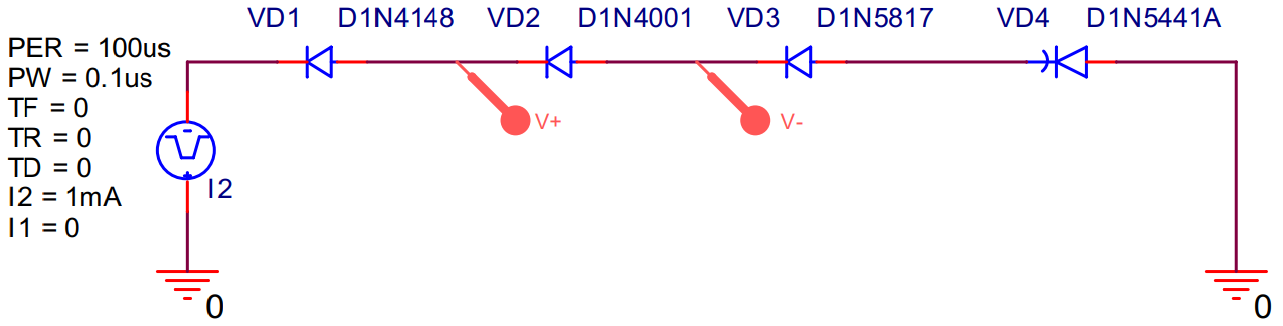
\includegraphics[width = 0.9 \textwidth]{scheme_1}
	\caption{\footnotesize Схема последовательного включения диодов}
	\vspace{1cm}
	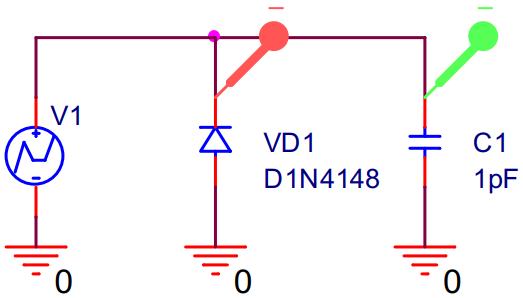
\includegraphics[width = 0.9 \textwidth]{scheme_2}
	\caption{\footnotesize Схема параллельного включения диодов}
	\label{scheme}
\end{figure}

\subsection*{2.1. Вольт-амперные характеристики}

\subsubsection*{Температурная зависимость обратной ветви ВАХ диода\\
$ I_{обр} = f(U_d, T = const) $}

\textbf{{\normalsize 2.1.1.}}
Получим зависимость токов заданного набора диодов от напряжения в диапазоне от $ -1V $ до $ 0.05V $ с шагом $ 1mV $ при температурах $ 17, 27, 37 $ градусов Цельсия.
Для температуры $ T = 27 \Cd $ запишем на графике каждого диода значение обратного тока при напряжении $ U_d = -0.1V $. Сравним с паспортными данными.

\begin{figure}[H]
	\centering
	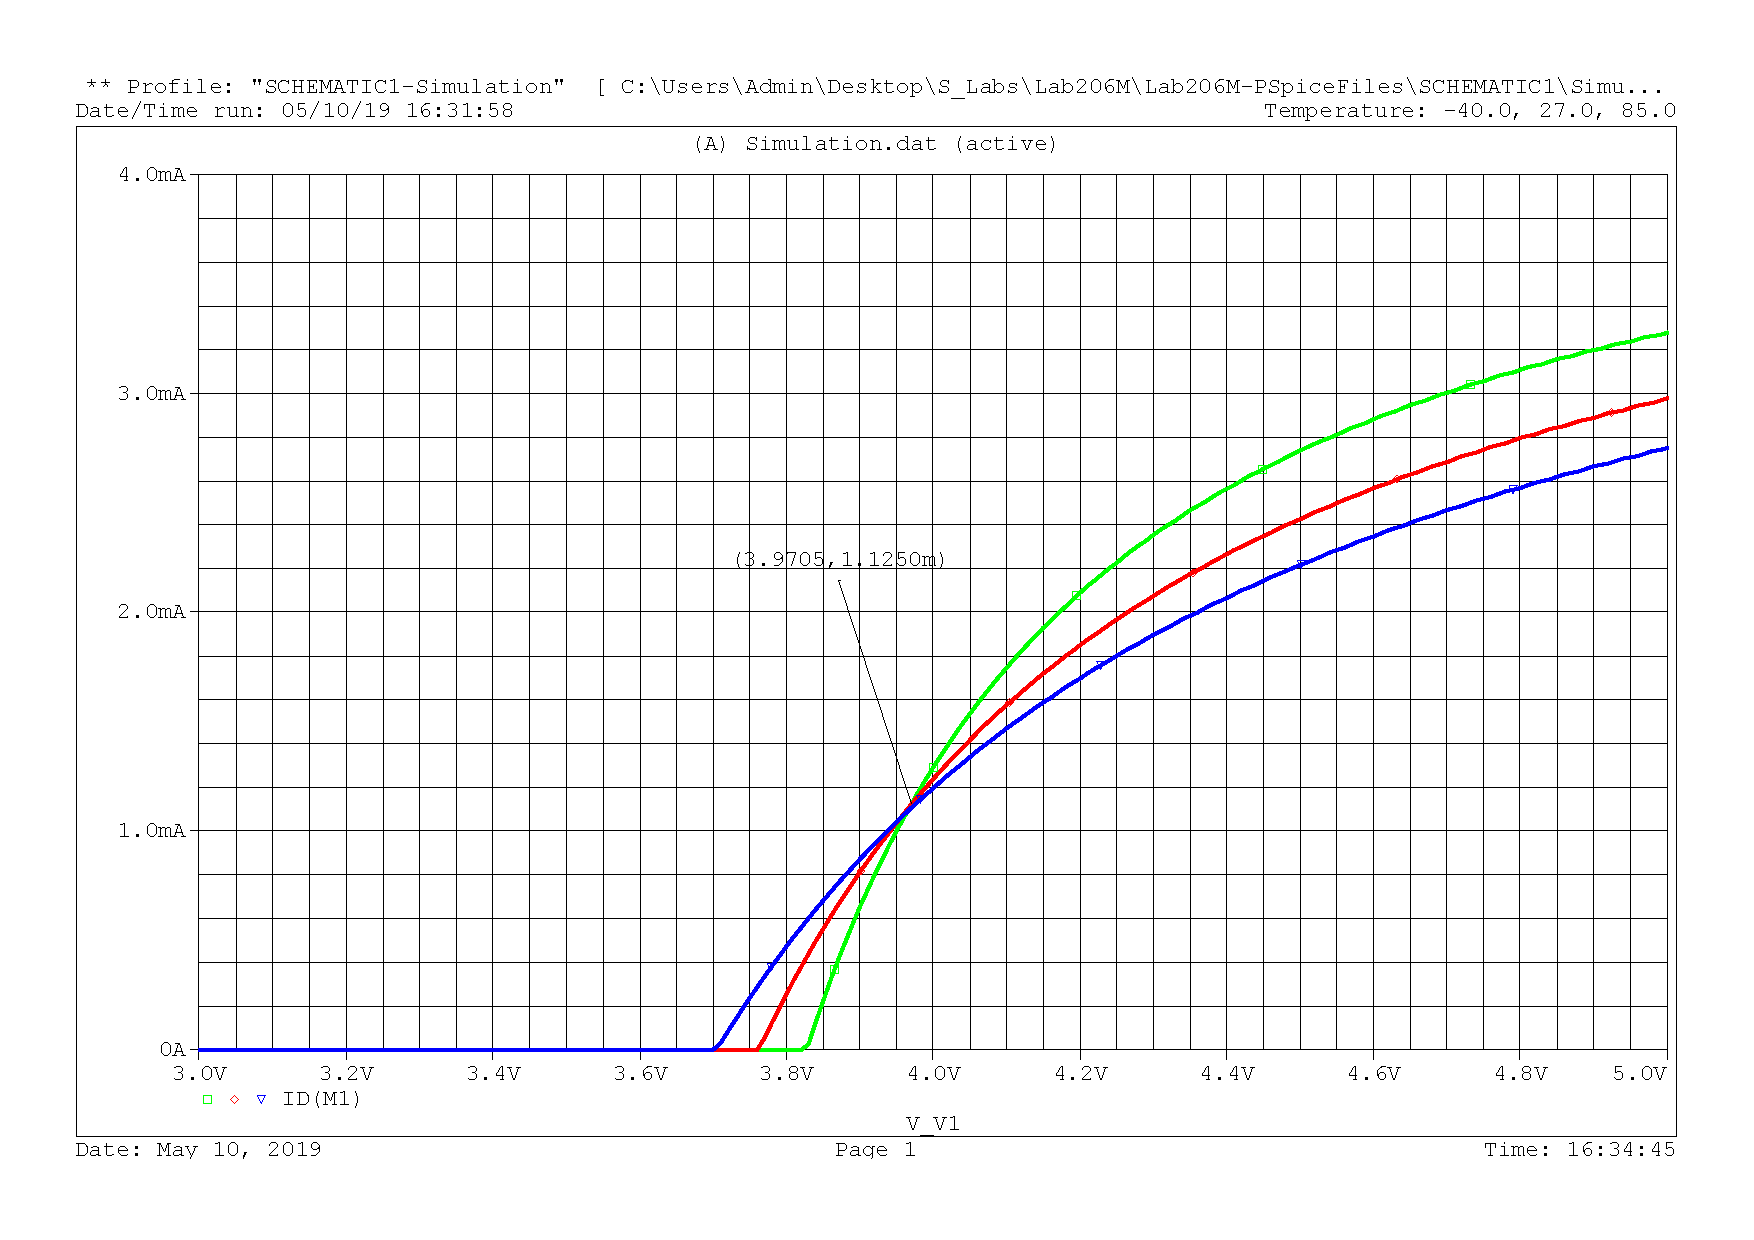
\includegraphics[width = 0.83 \textwidth]{1}
	\caption{D1N4149: $ I_{обр} = -3.7787~nA $}
	\label{2.1.1_1}
\end{figure}

\begin{figure}[H]
	\centering
	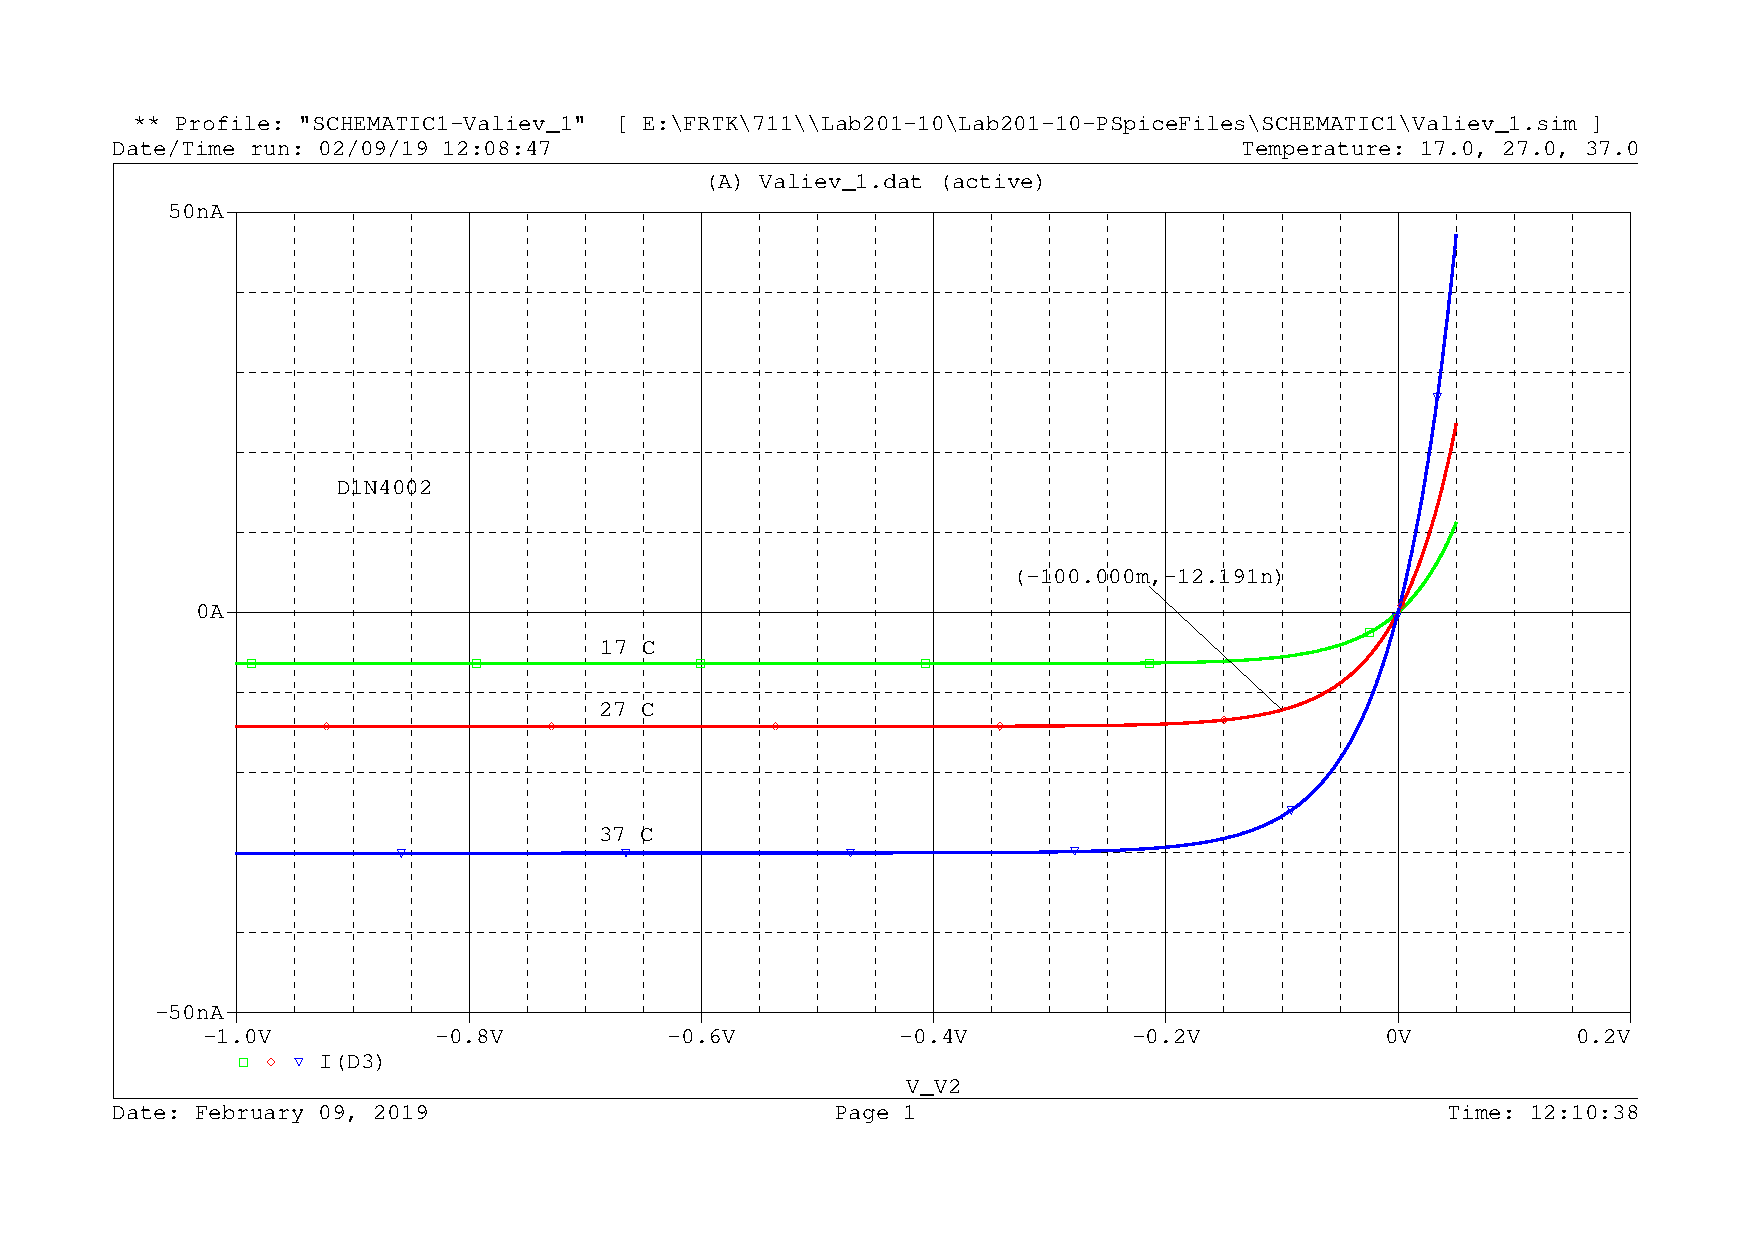
\includegraphics[width = 0.83 \textwidth]{2}
	\caption{D1N4002: $ I_{обр} = -12.191~nA $}
	\label{2.1.1_2}
\end{figure}

\begin{figure}[H]
	\centering
	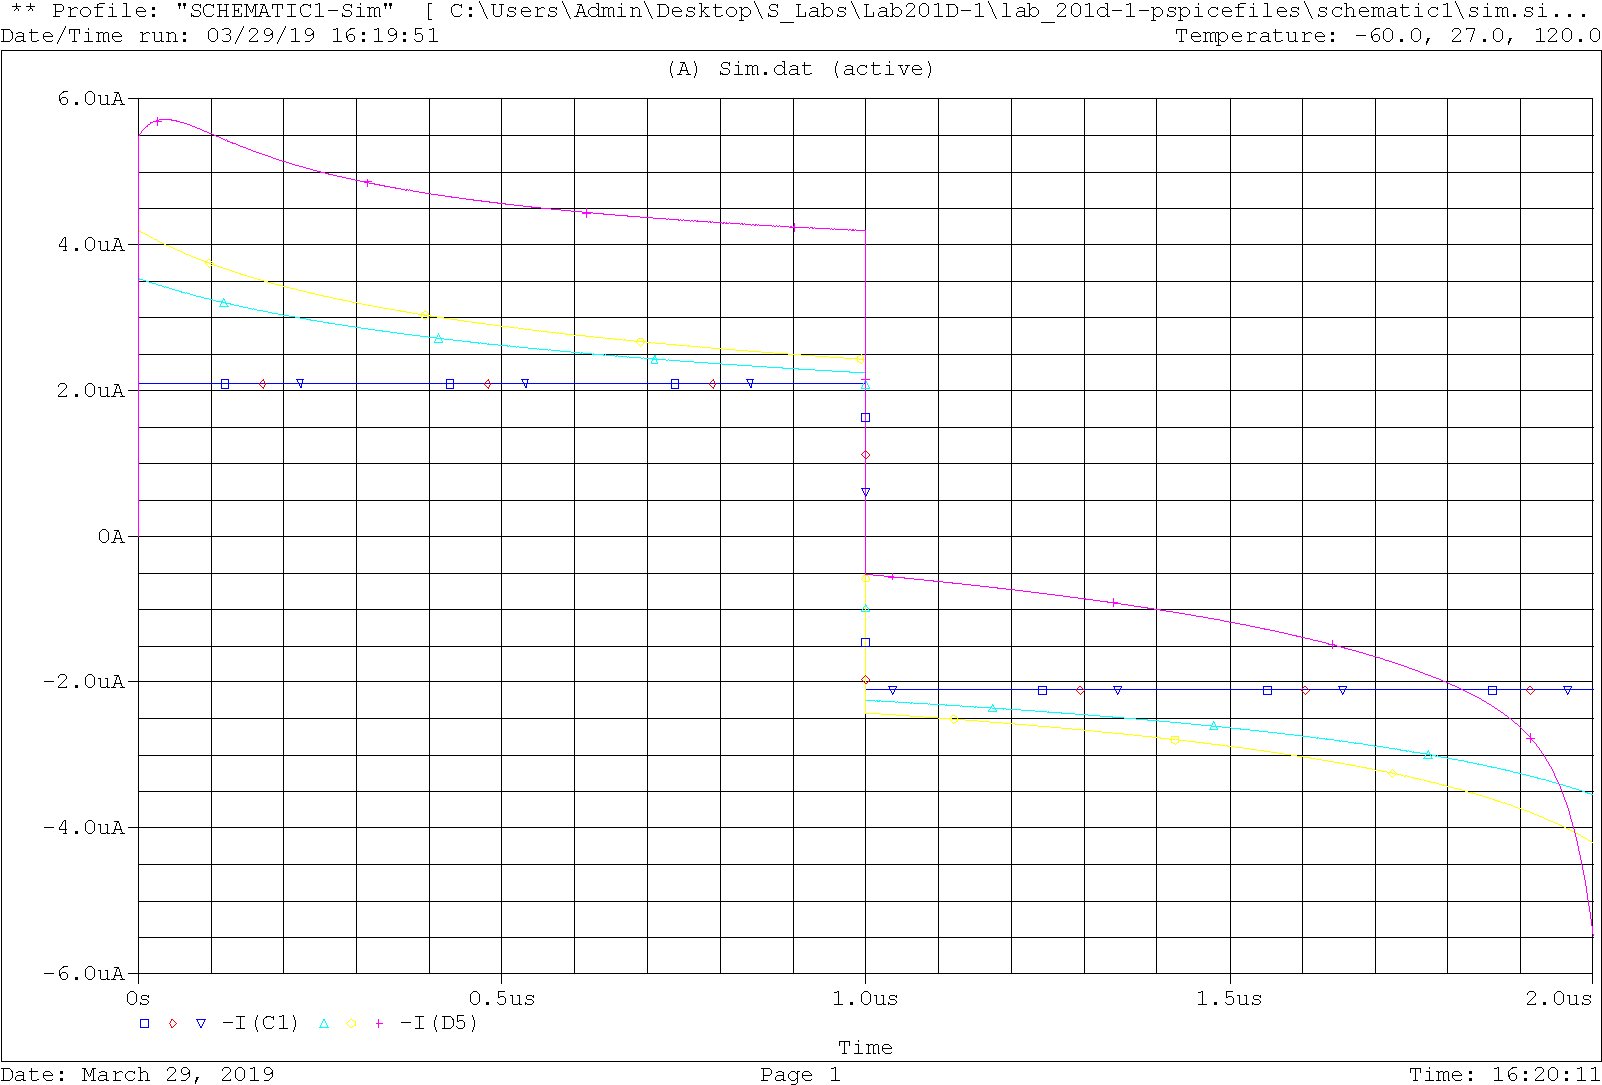
\includegraphics[width = 1 \textwidth]{3}
	\caption{D1N5818: $ I_{обр} = -27.360~uA $}
	\label{2.1.1_3}
\end{figure}

\begin{figure}[H]
	\centering
	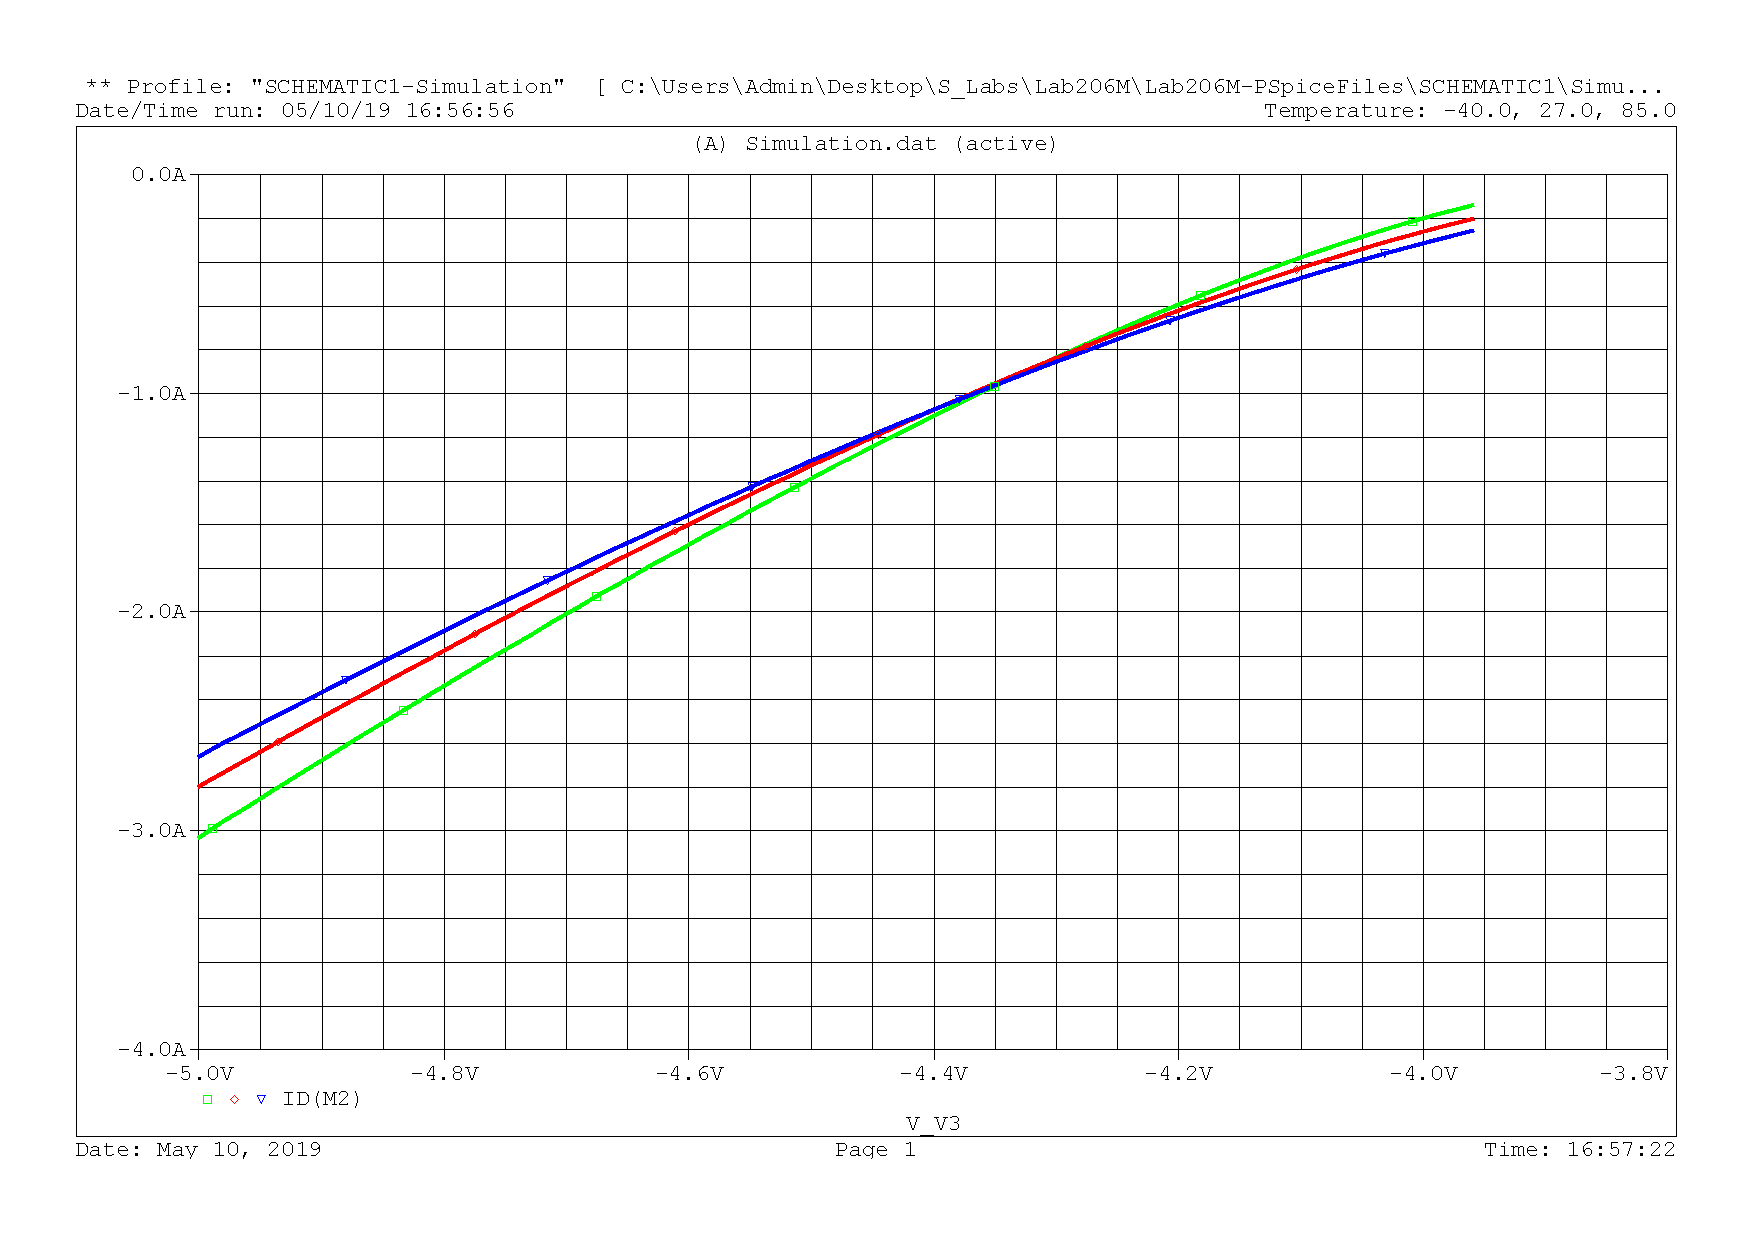
\includegraphics[width = 1 \textwidth]{4}
	\caption{D1N5443A: $ I_{обр} = -11.593~pA $}
	\label{2.1.1_4}
\end{figure}

\begin{figure}[H]
	\centering
	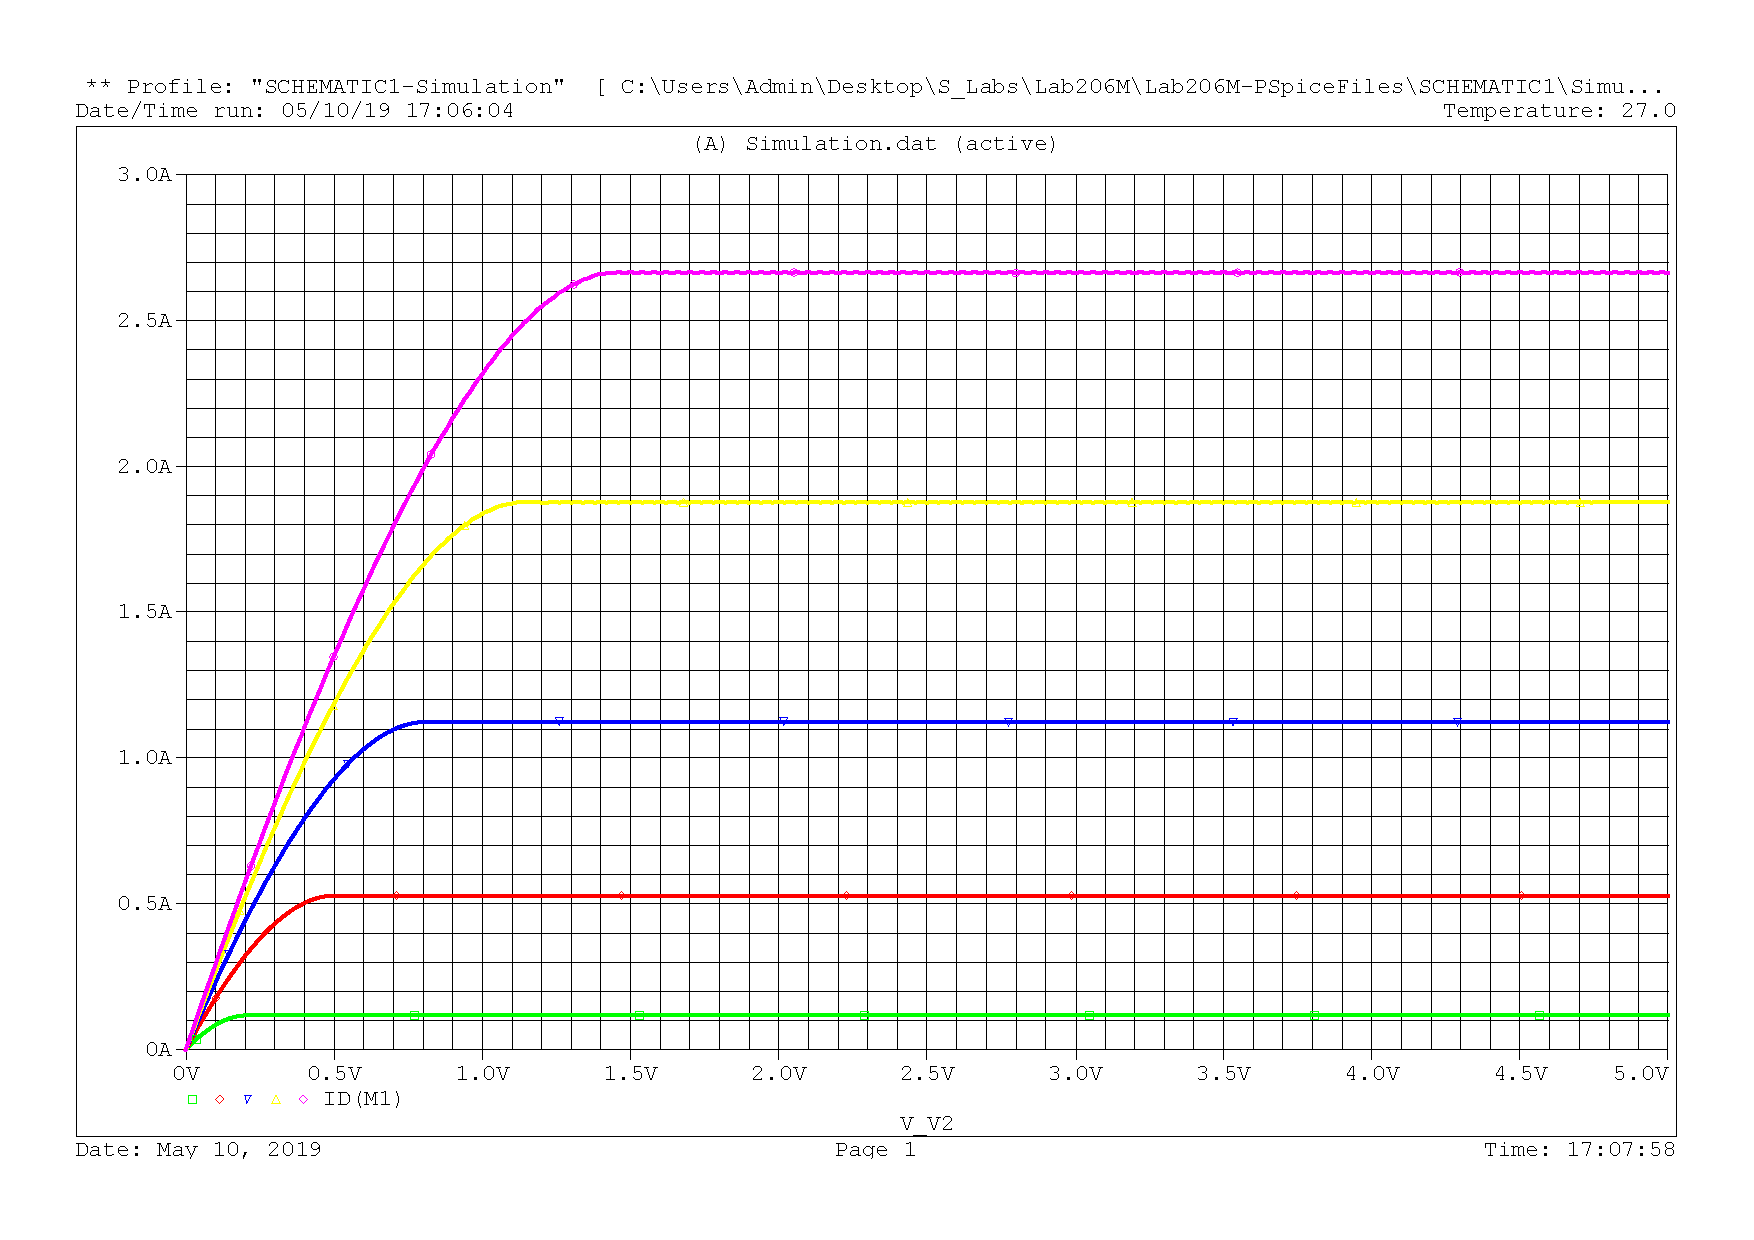
\includegraphics[width = 0.9 \textwidth]{5}
	\caption{D04AZ2\_2: $ I_{обр} = -85.940~uA $}
	\label{2.1.1_5}
\end{figure}

\textbf{{\normalsize 2.1.1.а.}}
Для импульсного ВЧ диода напечатаем значения обратных токов также для напряжения $ U_d = -1V $ и рассчитаем абсолютный и относительный температурные коэффициенты обратного тока для температуры $ T = 27 \Cd $:
\begin{equation}\label{eq:temperature}
абс.~ТКОТ = \ddc{I_{обр}(T)}{T}{U} \left[ A/\Cd \right] ~~~
относ.~ТКОТ = \dfrac{абс.~ТКОТ (T)}{I_{обр}(T)} \cdot 100 \left[ \%/\Cd \right]
\end{equation}

\begin{figure}[H]
	\centering
	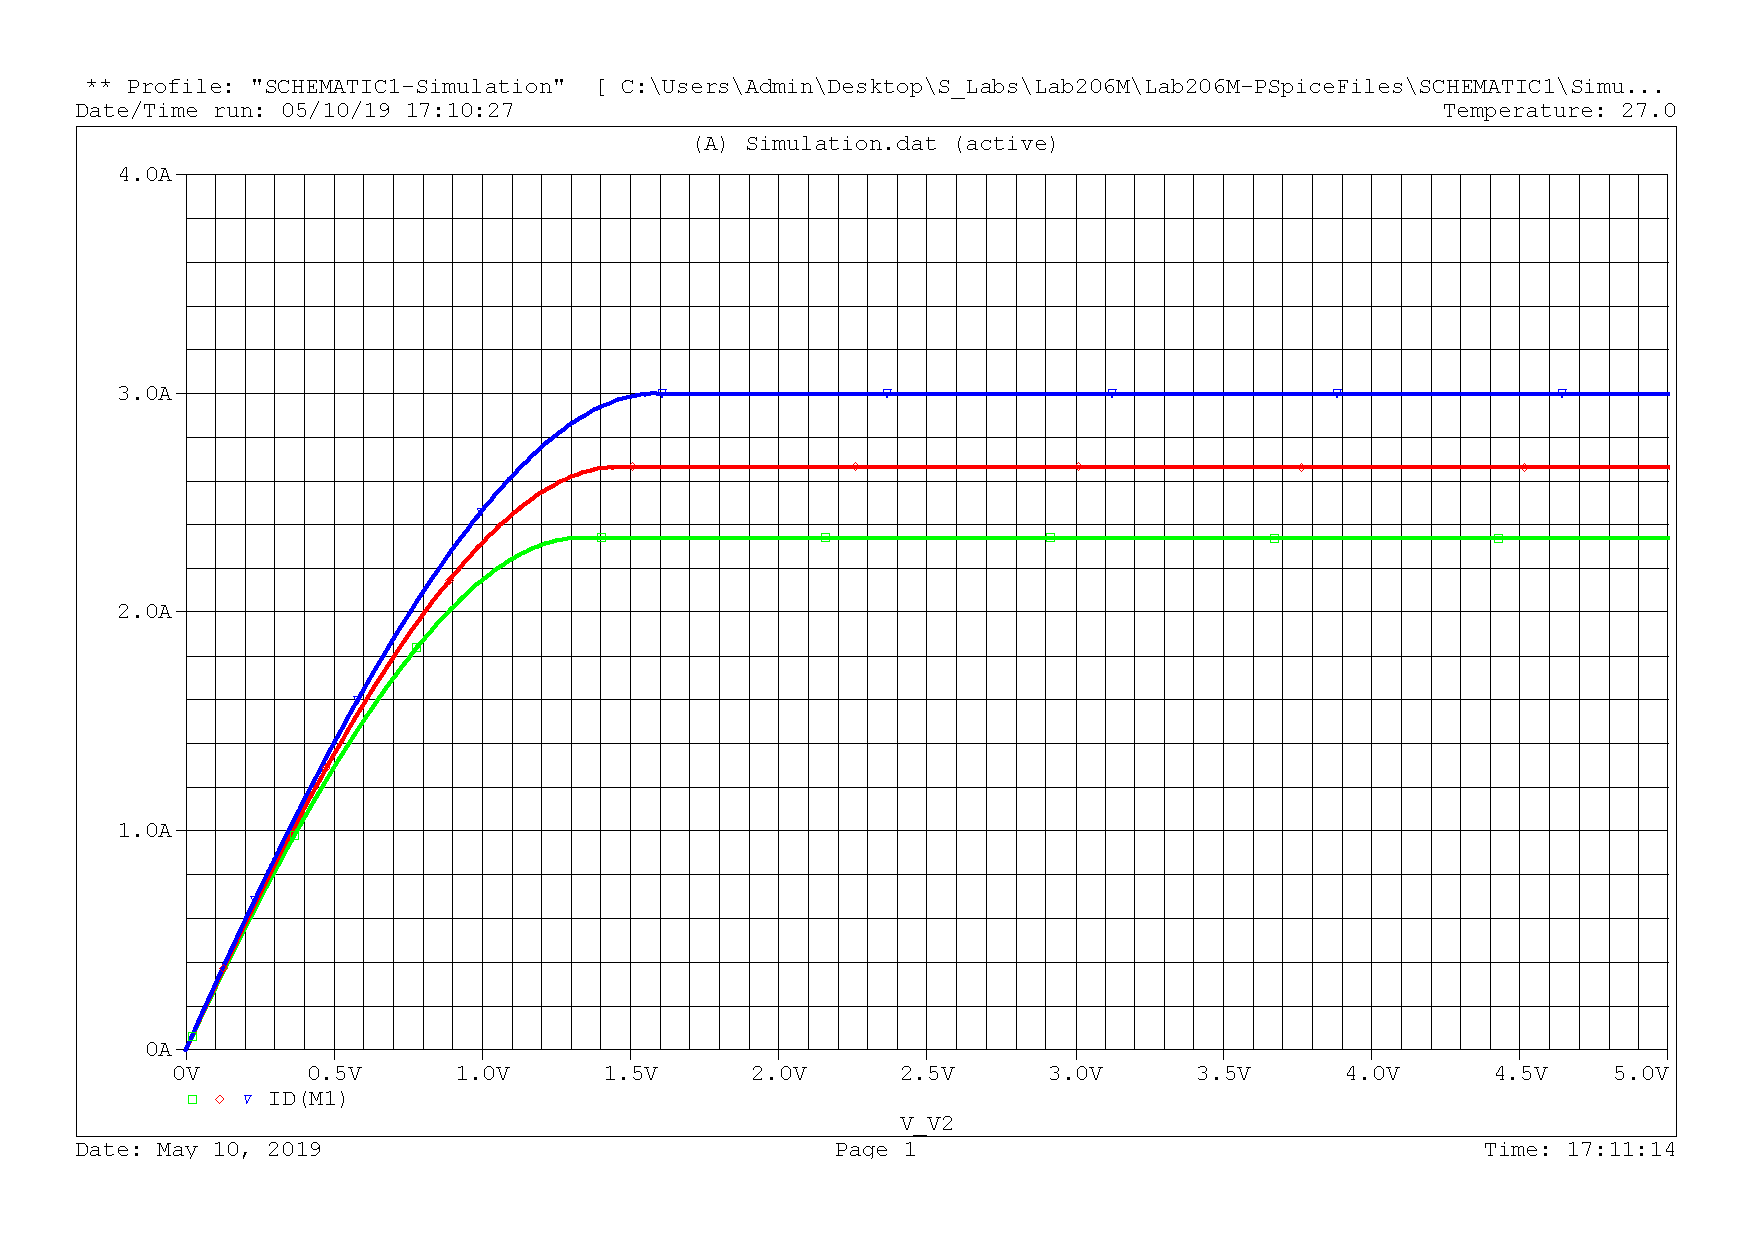
\includegraphics[width = 0.9 \textwidth]{6}
	\caption{D1N4149: $ абс.ТКОТ = -398.710~pA/\Cd $ и $ относ.~ТКОТ = 8~\%/\Cd $}
	\label{2.1.1.1}
\end{figure}

\textbf{{\normalsize 2.1.1.б.}}
Рассчитаем обратный ток диода при $ T = 47\Cd $, используя примерную температуру удвоения $ \Delta T = 10\Cd $.
\begin{equation}\label{eq:2.1.1.2}
I_{обр}(T = 47\Cd) = I_{обр}(T = 27\Cd) \cdot 4 = -3.7787~nA * 4 = 15.1148~nA
\end{equation}

\textbf{{\normalsize 2.1.1.в.}}
Рассчитаем фактическую температуру удвоения $ \Delta T_{факт} $.
\begin{equation}\label{eq:T_fact}
\Delta T_{факт} = \Delta T \cdot \dfrac{0.693}{\ln N} = 9.98 \Cd ~~~~~ где ~ N = \dfrac{I_{обр}(T + \Delta T)}{I_{обр}(T)}
\end{equation}

%\newpage

\subsubsection*{Температурная зависимость прямой ветви ВАХ диода\\
$ I_{пр} = f(U_d, T = const) $}

\textbf{{\normalsize 2.1.2.}}
Повторим получение токов диодов при тех же значениях температуры $ 17, 27, 37 $ градусов Цельсия, но в диапазоне положительных напряжений от $ +0.1V $ до $ +0.6V $ с шагом $ 1mV $.

\begin{figure}[H]
	\centering
	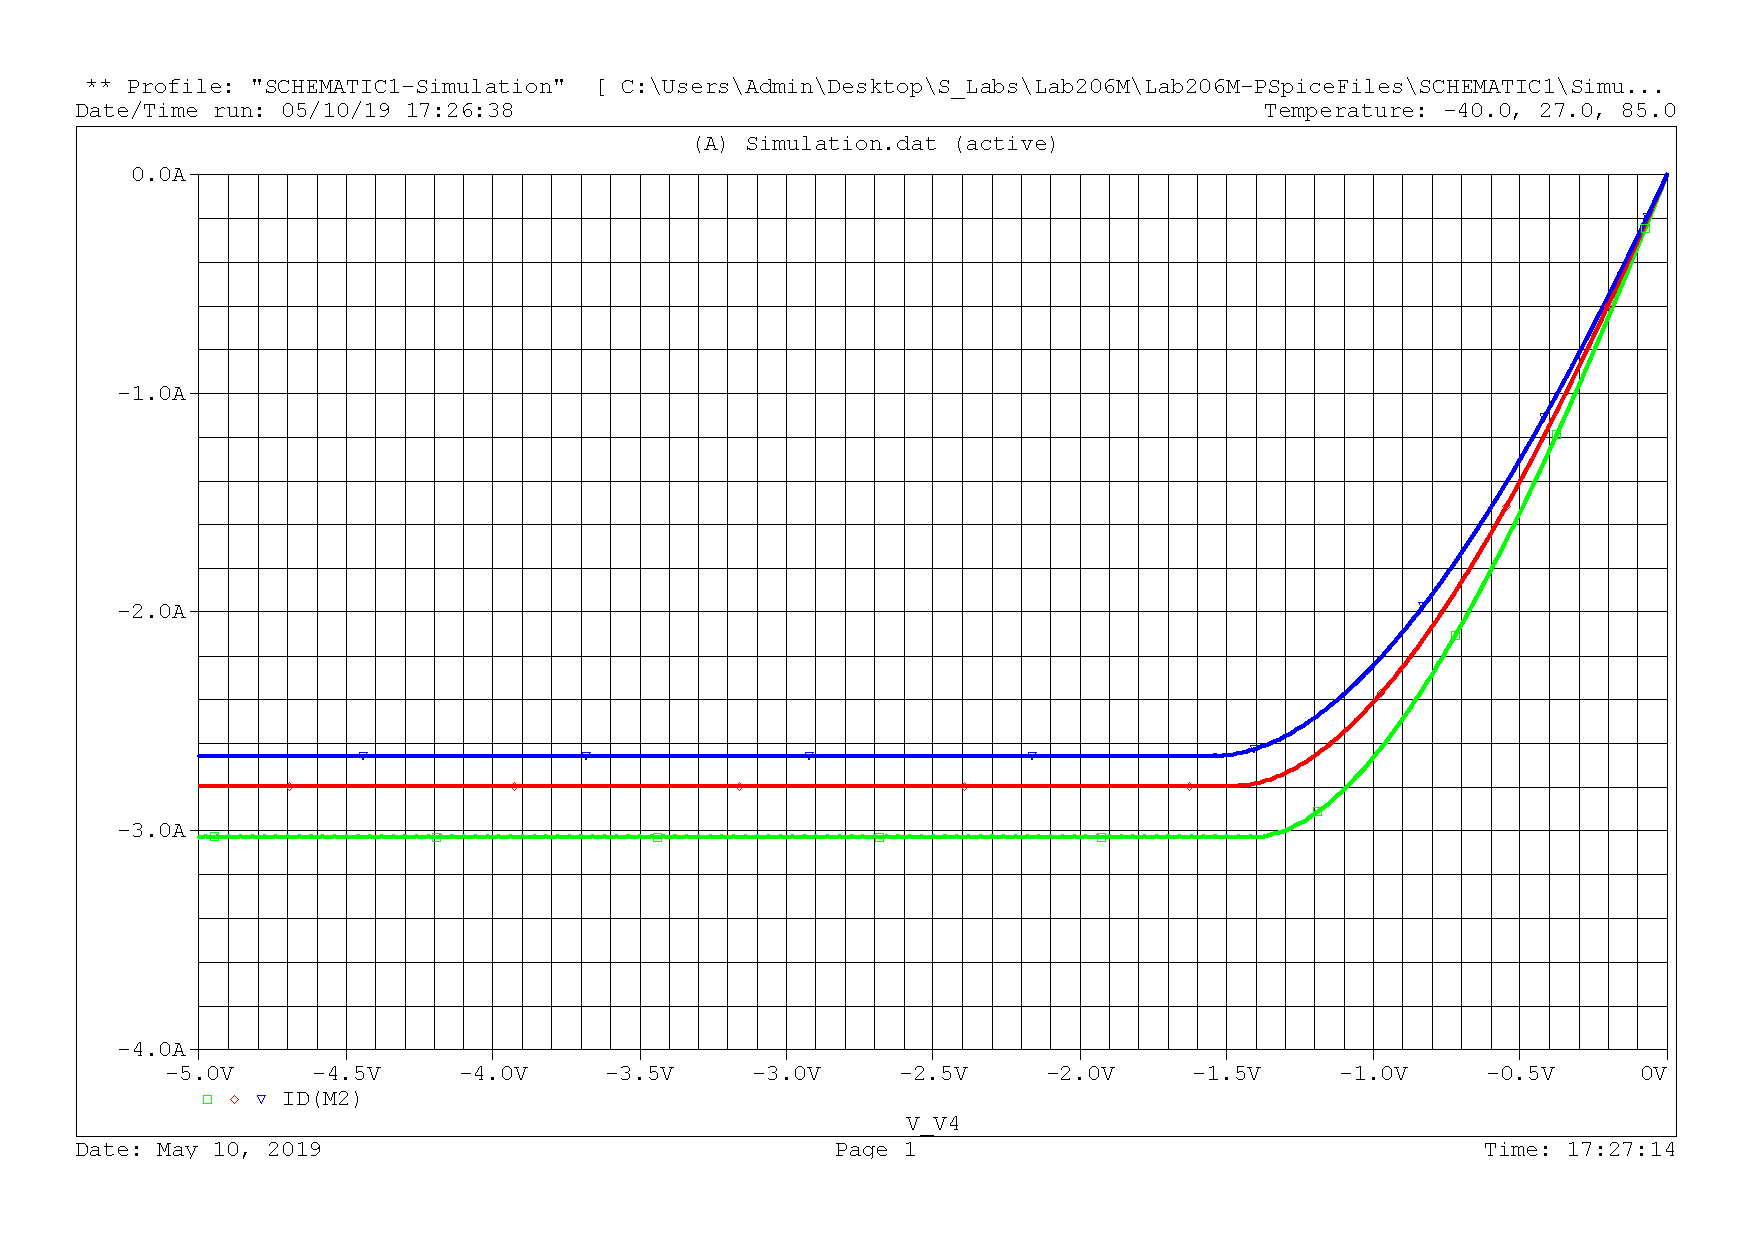
\includegraphics[width = \textwidth]{11}
	\caption{D1N4149}
	\label{2.1.2_1}
\end{figure}

\begin{figure}[H]
	\centering
	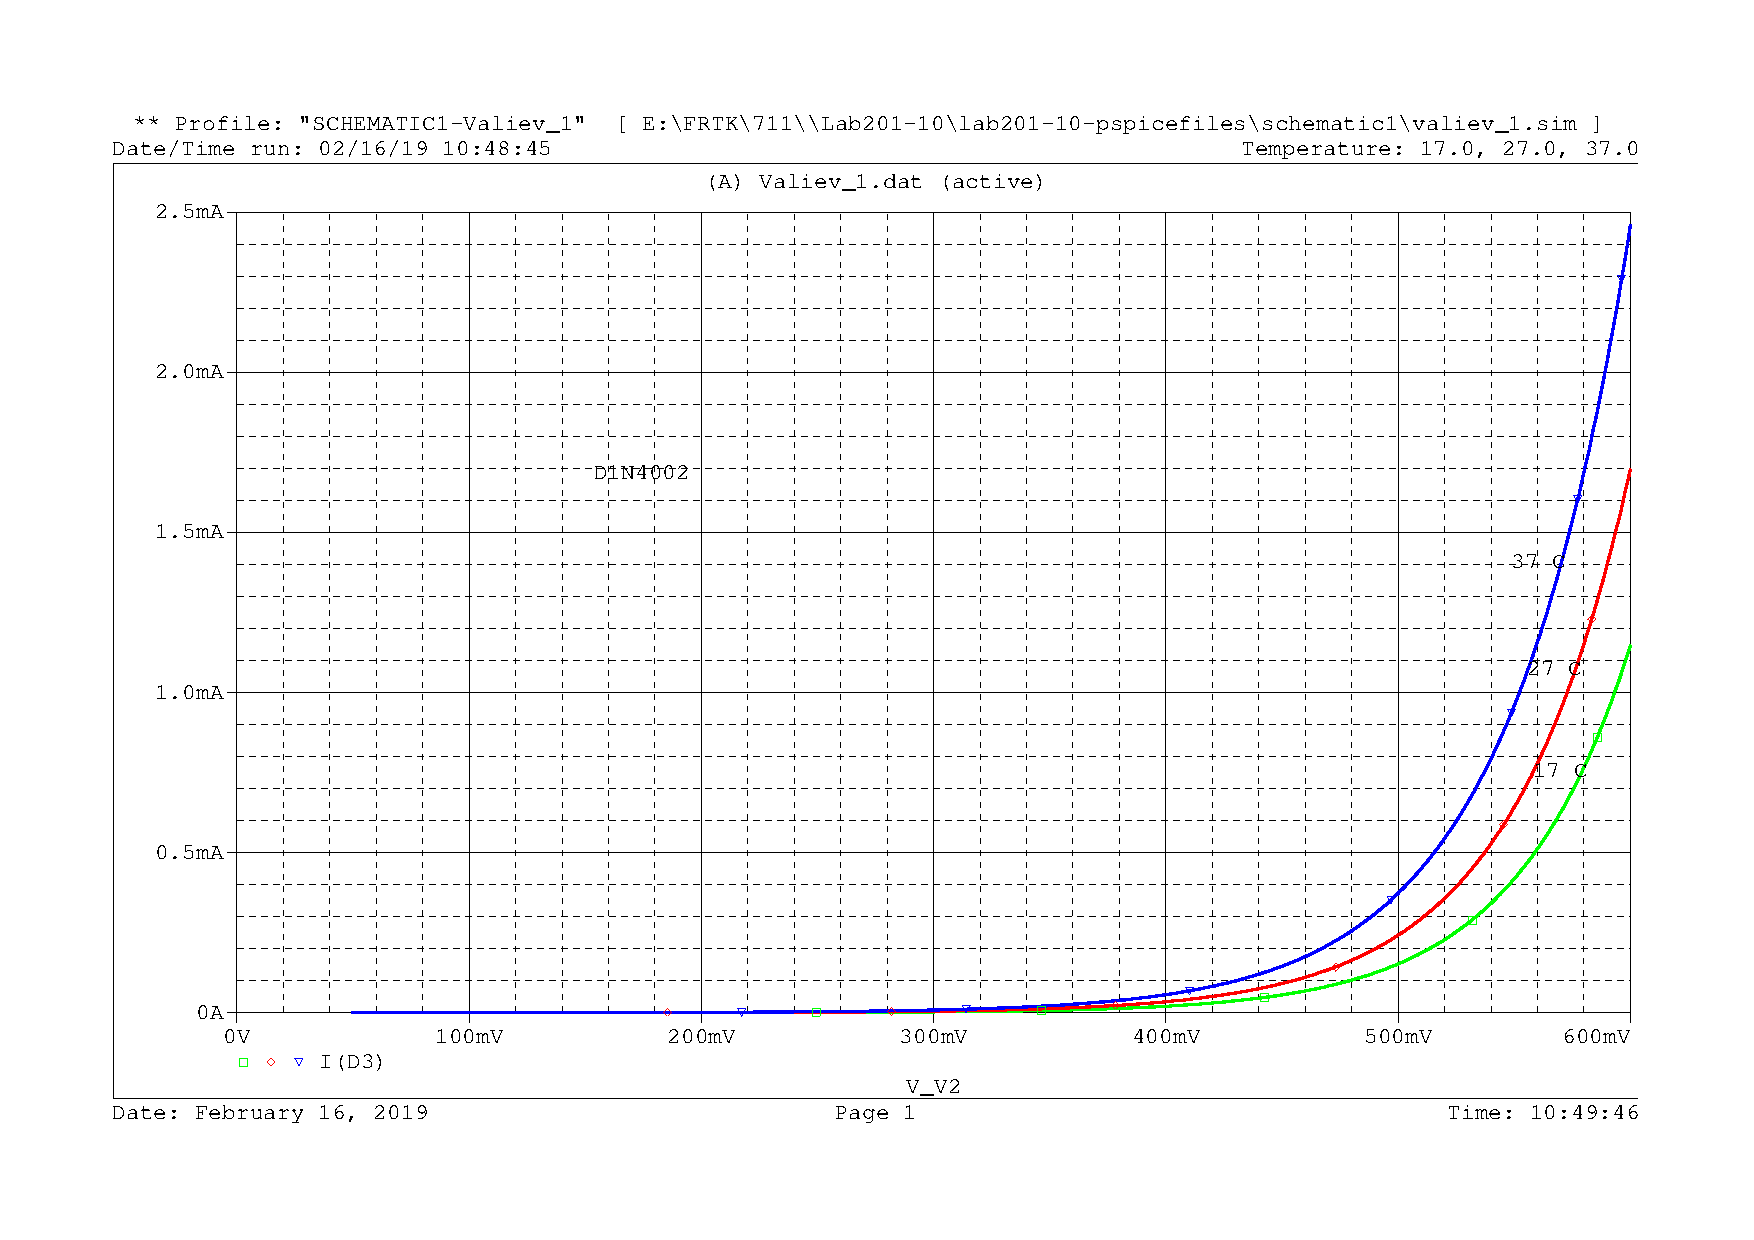
\includegraphics[width = \textwidth]{12}
	\caption{D1N4002}
	\label{2.1.2_2}
\end{figure}

\begin{figure}[H]
	\centering
	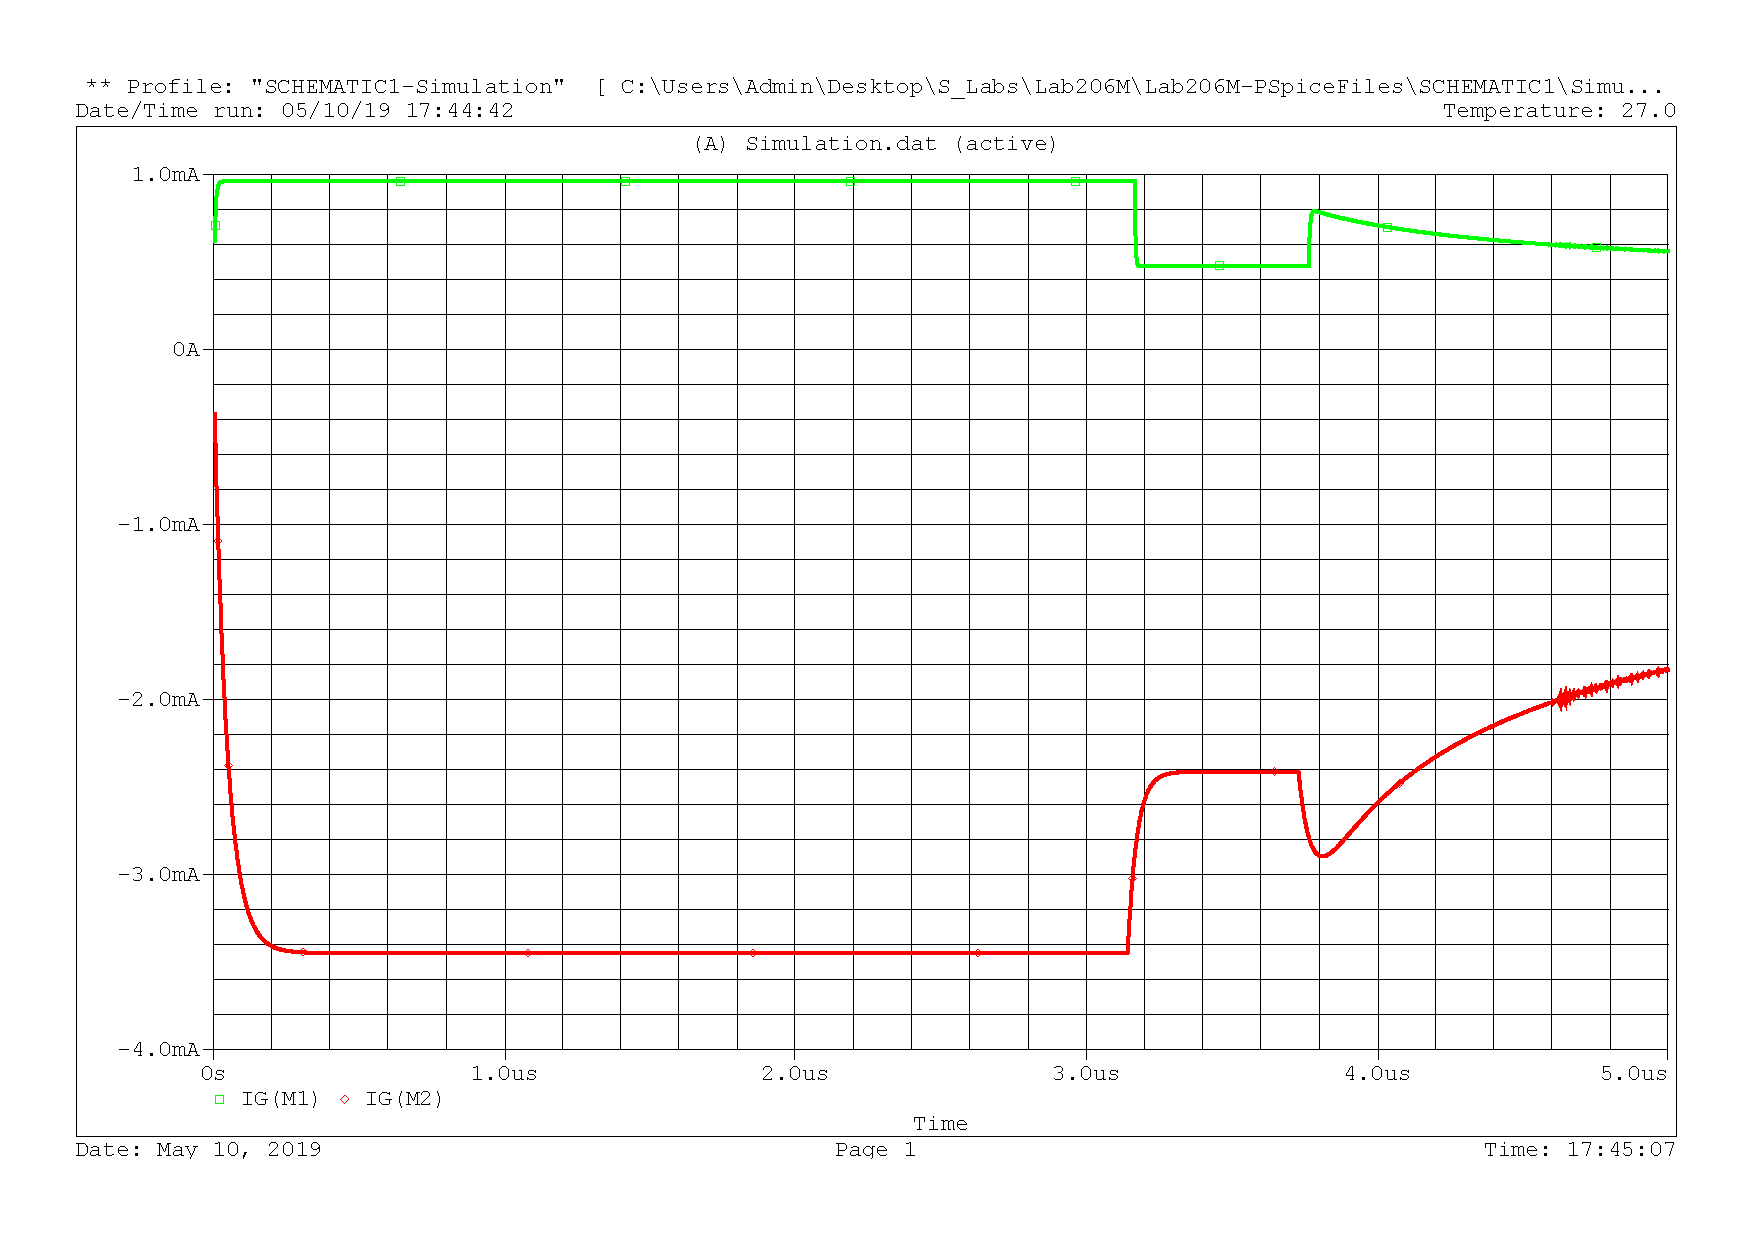
\includegraphics[width = \textwidth]{13}
	\caption{D1N5818}
	\label{2.1.2_3}
\end{figure}

\begin{figure}[H]
	\centering
	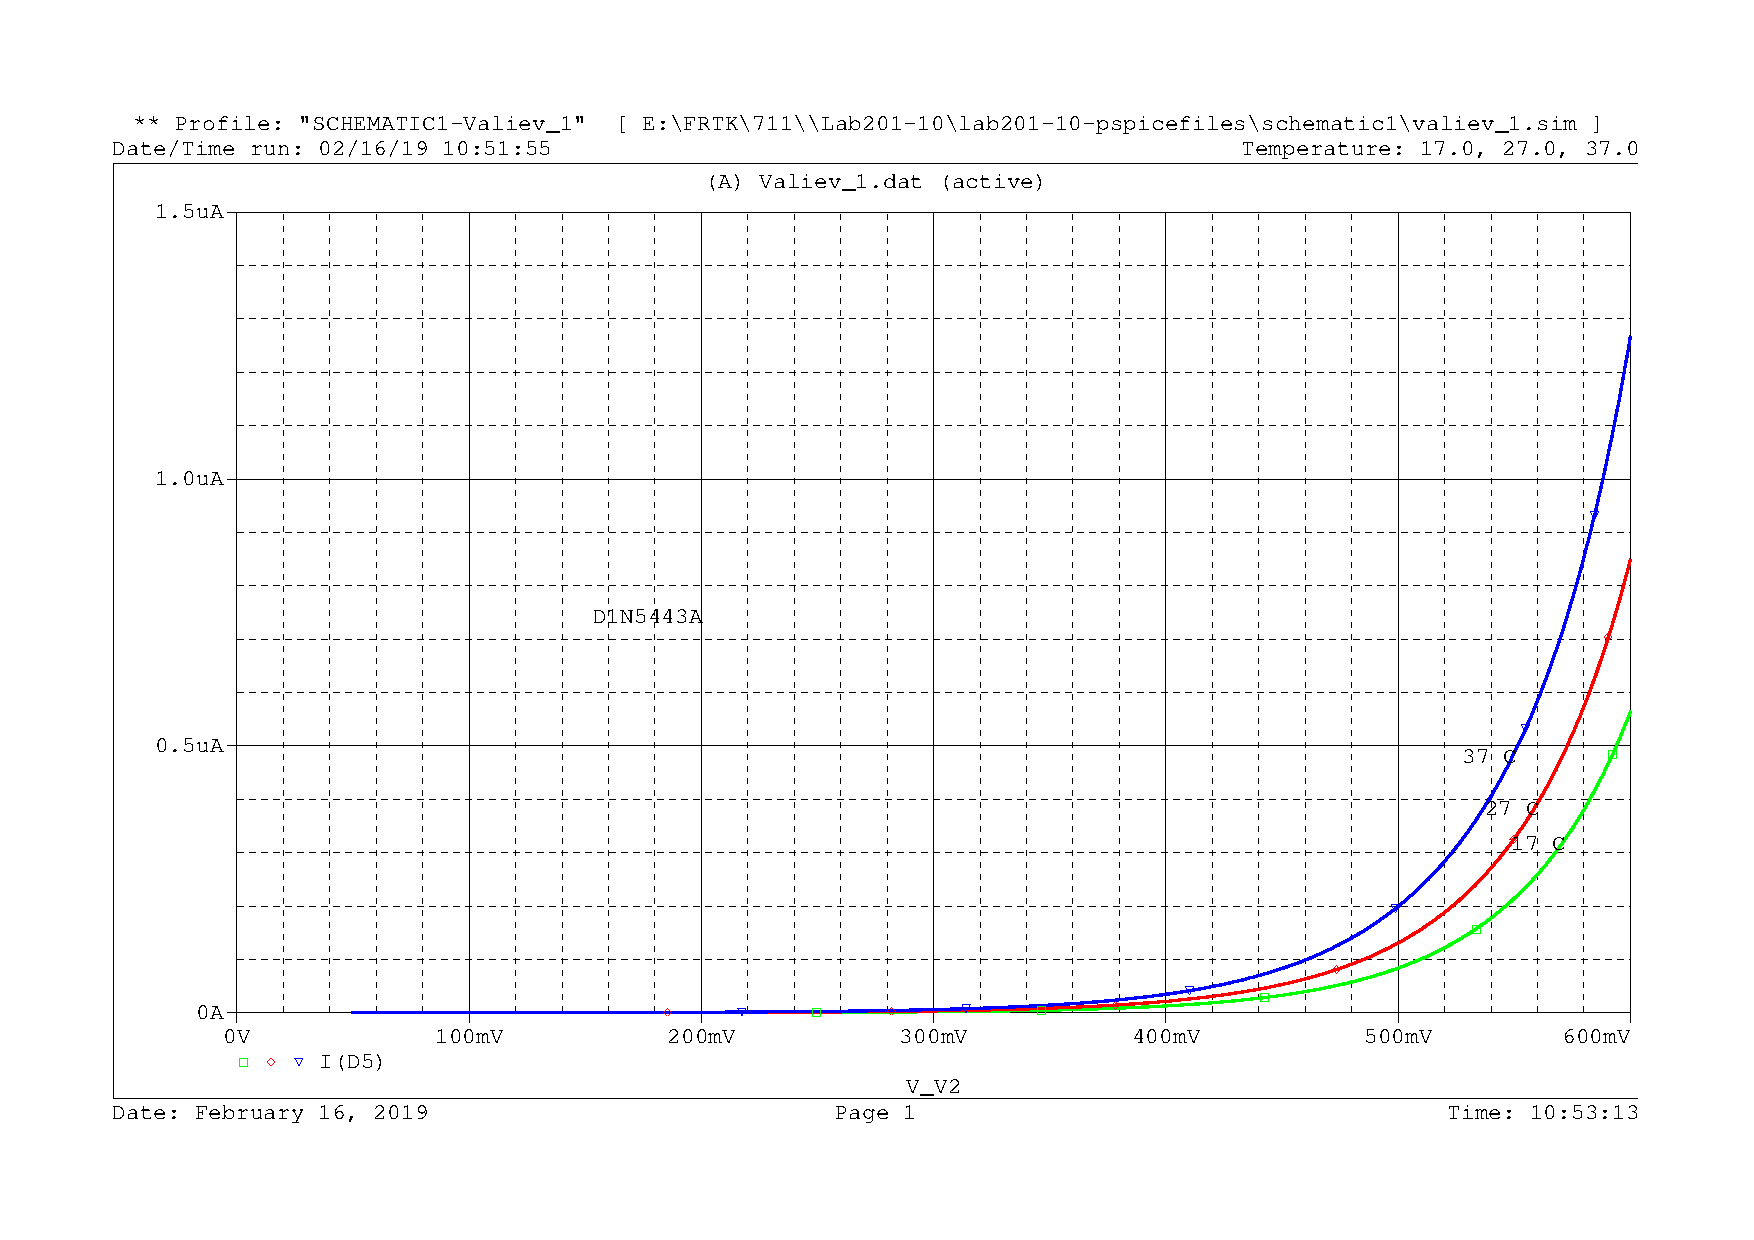
\includegraphics[width = \textwidth]{14}
	\caption{D1N5443A}
	\label{2.1.2_4}
\end{figure}

\begin{figure}[H]
	\centering
	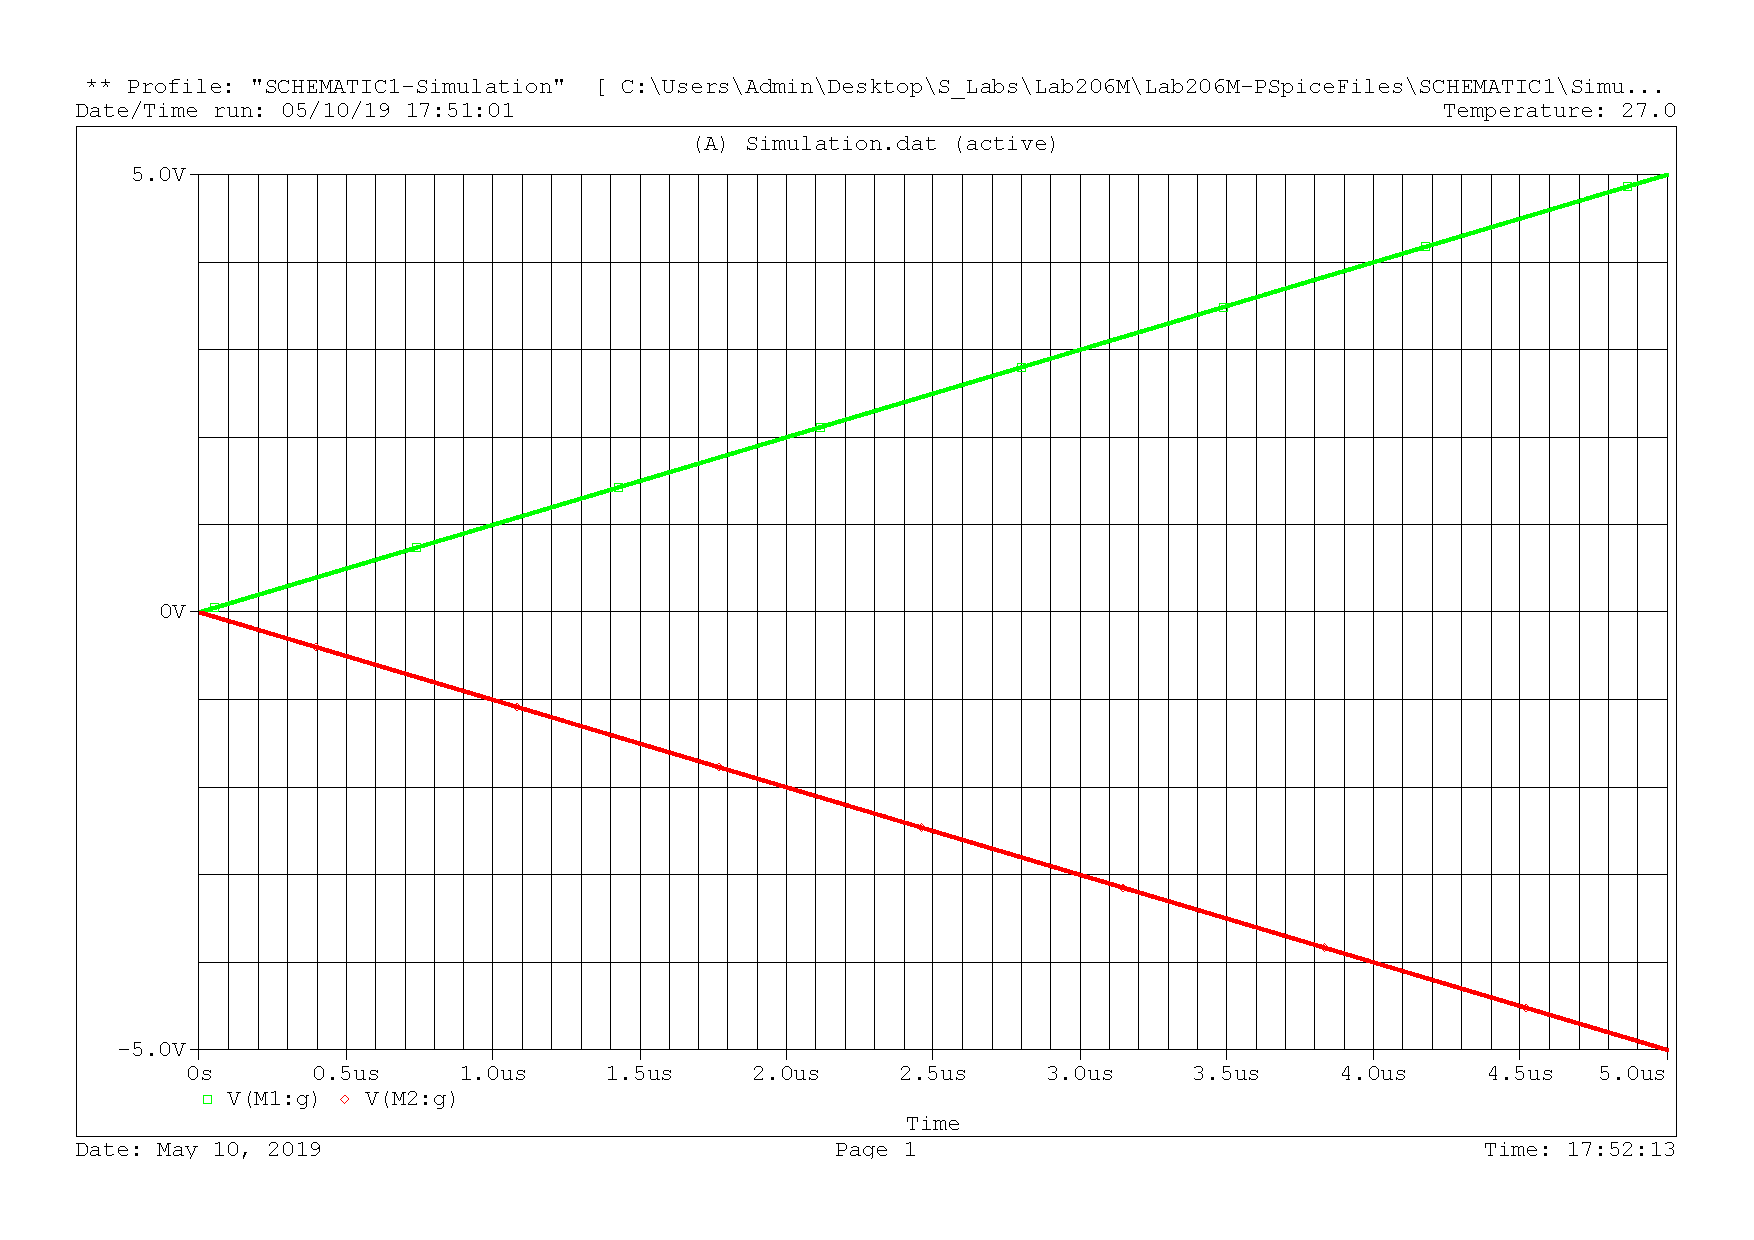
\includegraphics[width = \textwidth]{15}
	\caption{D04AZ2\_2}
	\label{2.1.2_5}
\end{figure}

\newpage

\textbf{{\normalsize 2.1.2.а.}}
Напечатаем на графике для импульсного ВЧ диода значения токов при напряжении $ U_d = 0.6V $.

\begin{figure}[H]
	\centering
	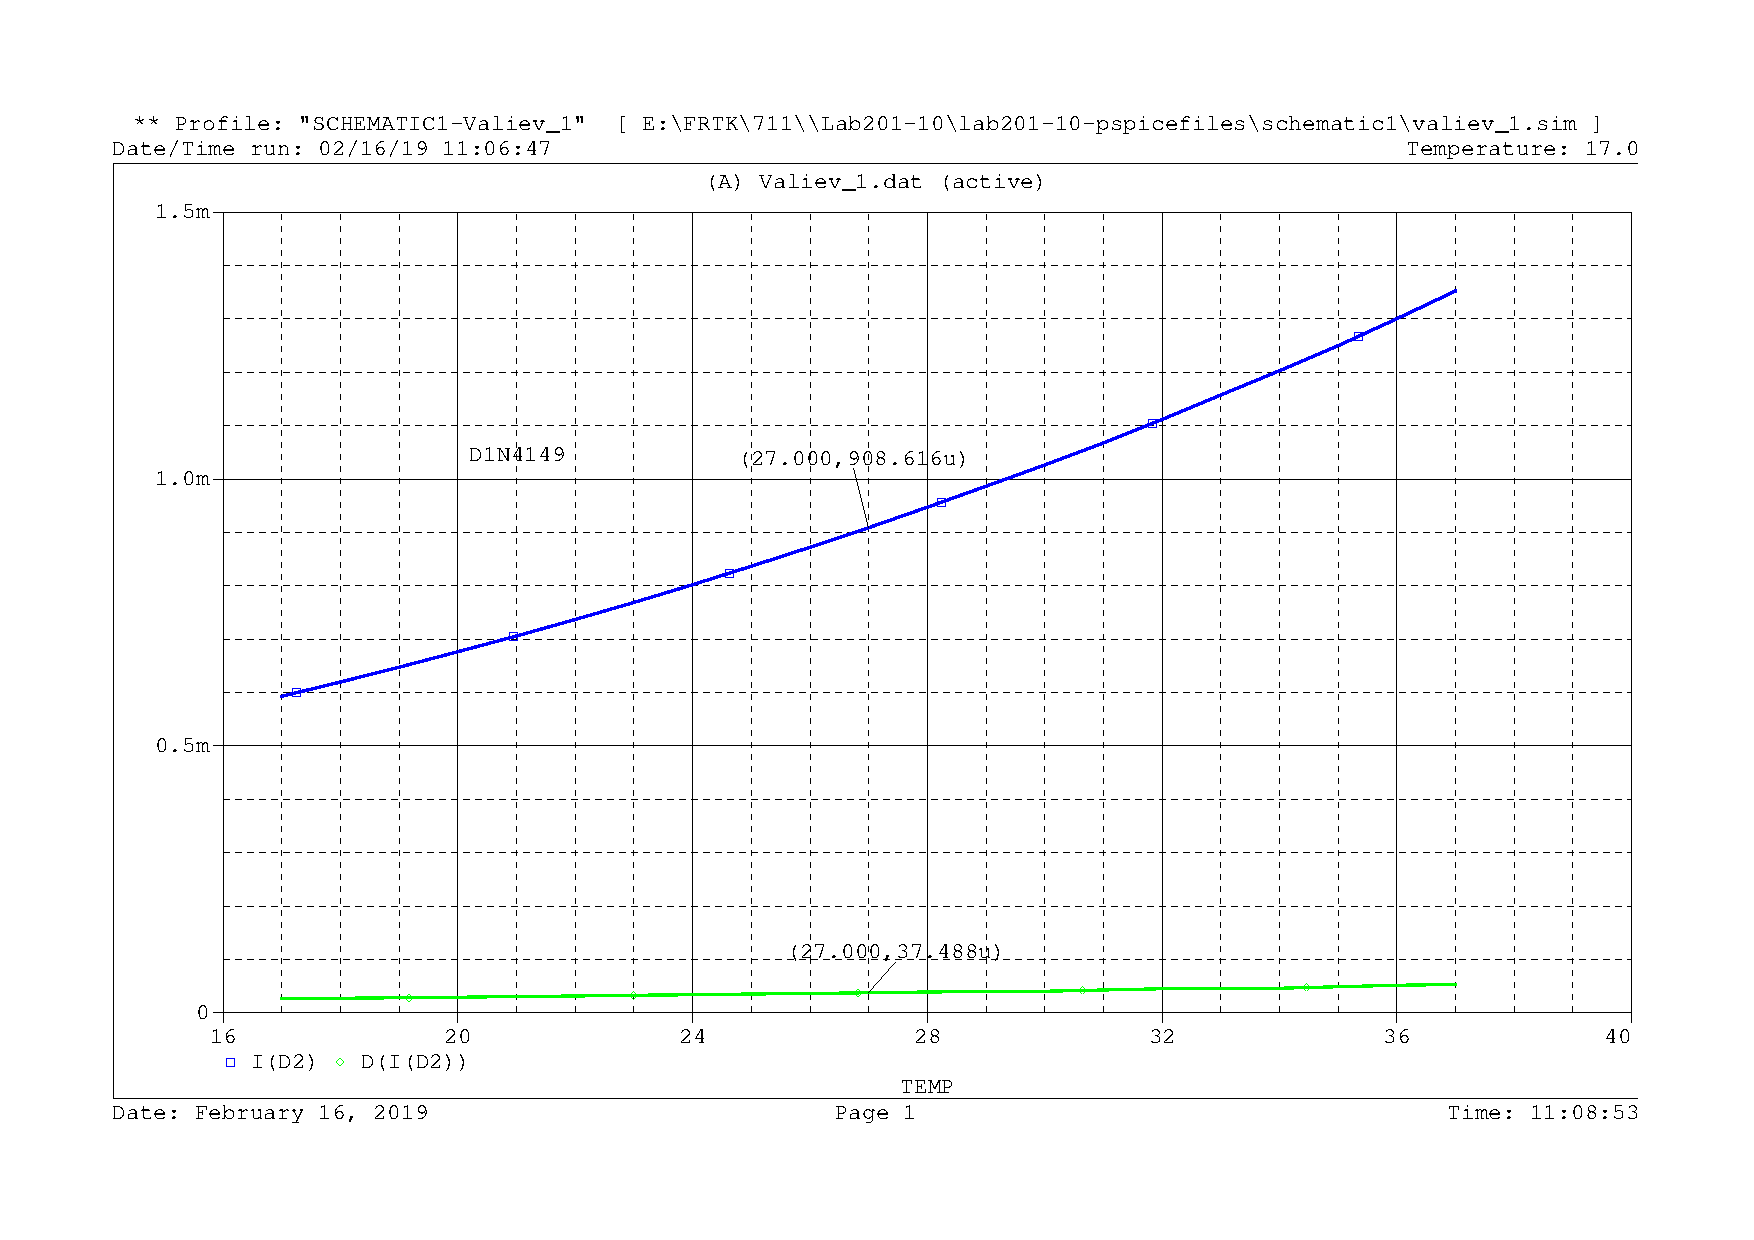
\includegraphics[width = \textwidth]{16}
	\caption{D1N4149: $ относ.~ТКОТ = 4.1\% $}
	\label{2.1.2.2}
\end{figure}

\newpage

\subsubsection*{Прямая ВАХ диода в полулогарифмических координатах}

\textbf{{\normalsize 2.1.3.}}
Получим на одном графике в логарифмическом масштабе зависимости токов от напряжения всех диодов заданного набора в диапазоне от $ +0.05V $ до $ +5V $ при температуре $ T = 27 \Cd $.

\begin{figure}[H]
	\centering
	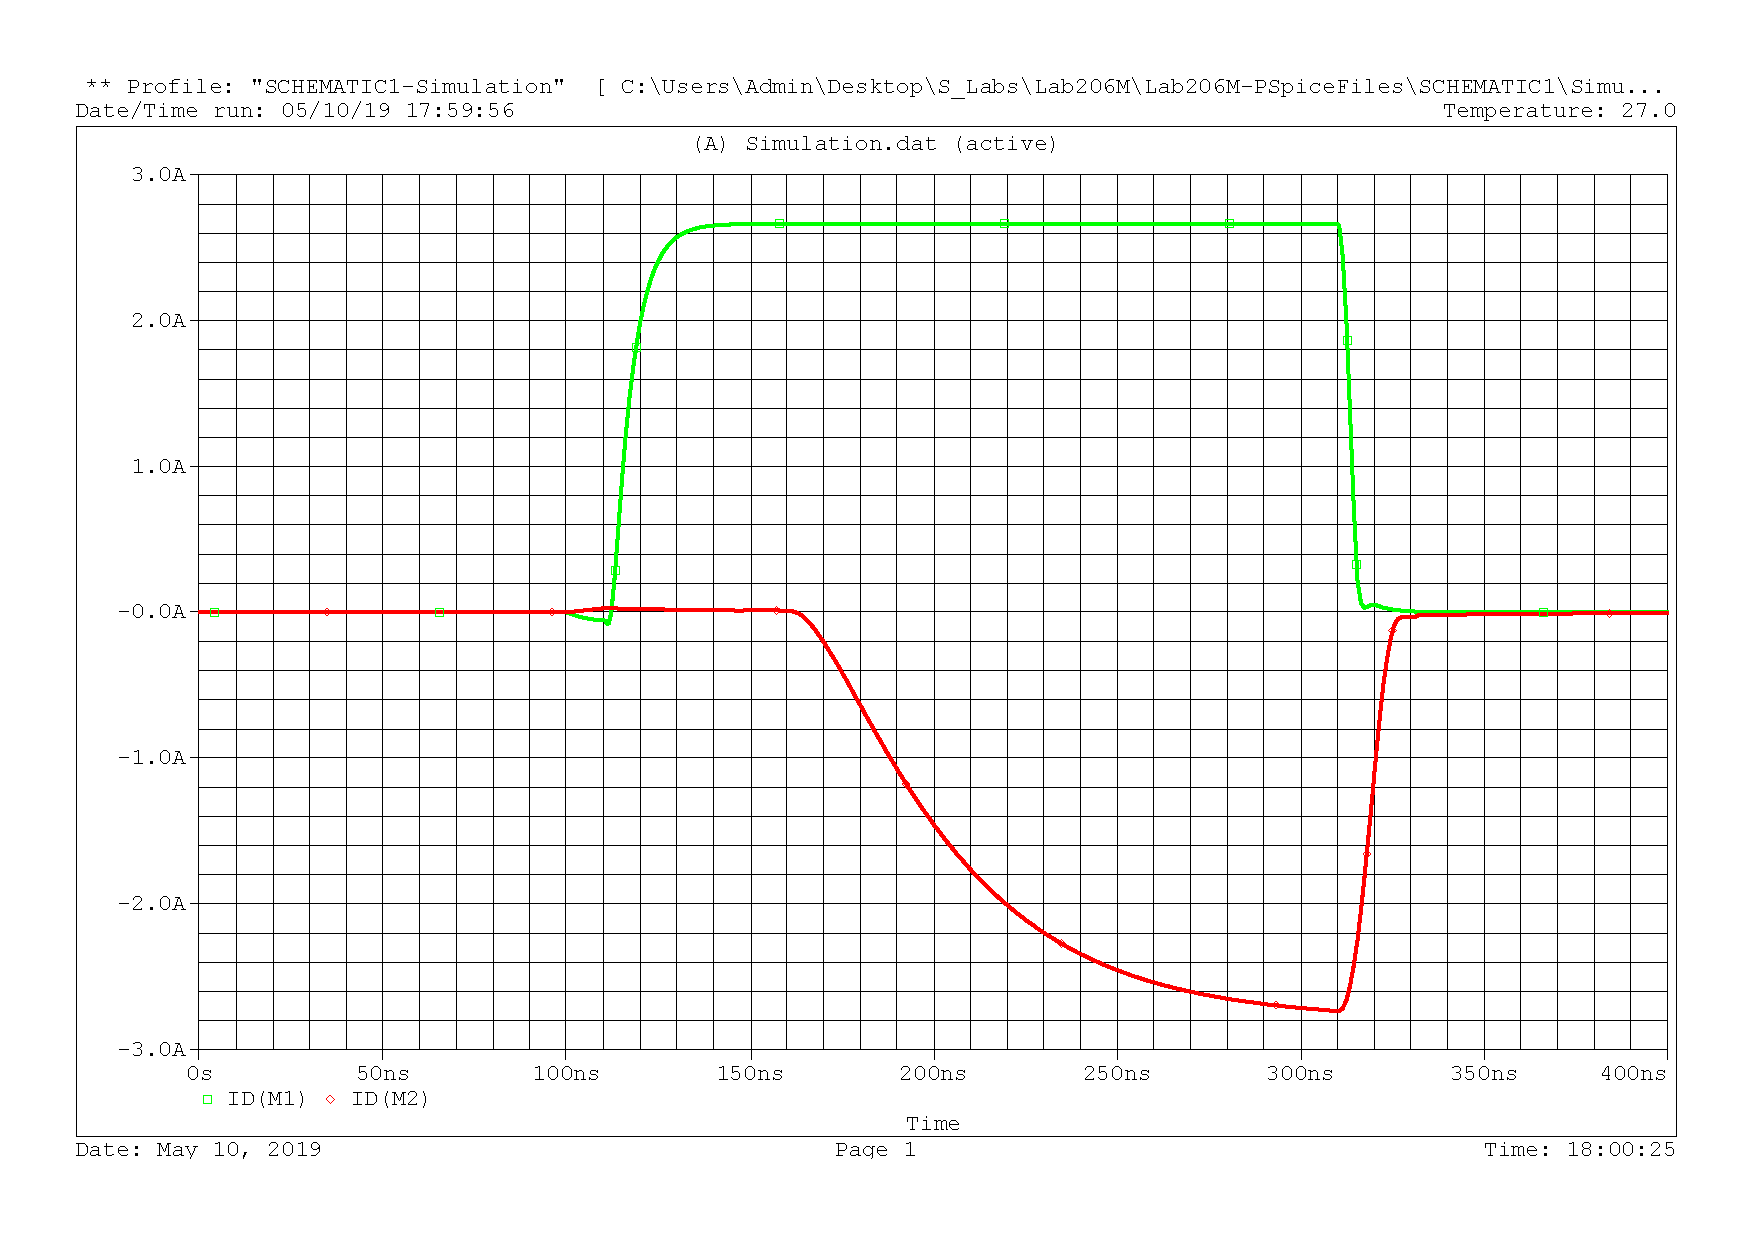
\includegraphics[width = 0.85 \textwidth]{17}
	\caption{Список диодов на представлен по порядку, показанному снизу для линий}
	\label{2.1.3}
\end{figure}

\textbf{{\normalsize 2.1.3.а.}}
Для импульсного ВЧ диода получим в логарифмическом масштабе семейство температурно-зависимых ВАХ прямого тока $ I_{пр} = f(U_d, T = const) $\\
при $ -40\Cd,~27\Cd,~85\Cd $.

\begin{figure}[H]
	\centering
	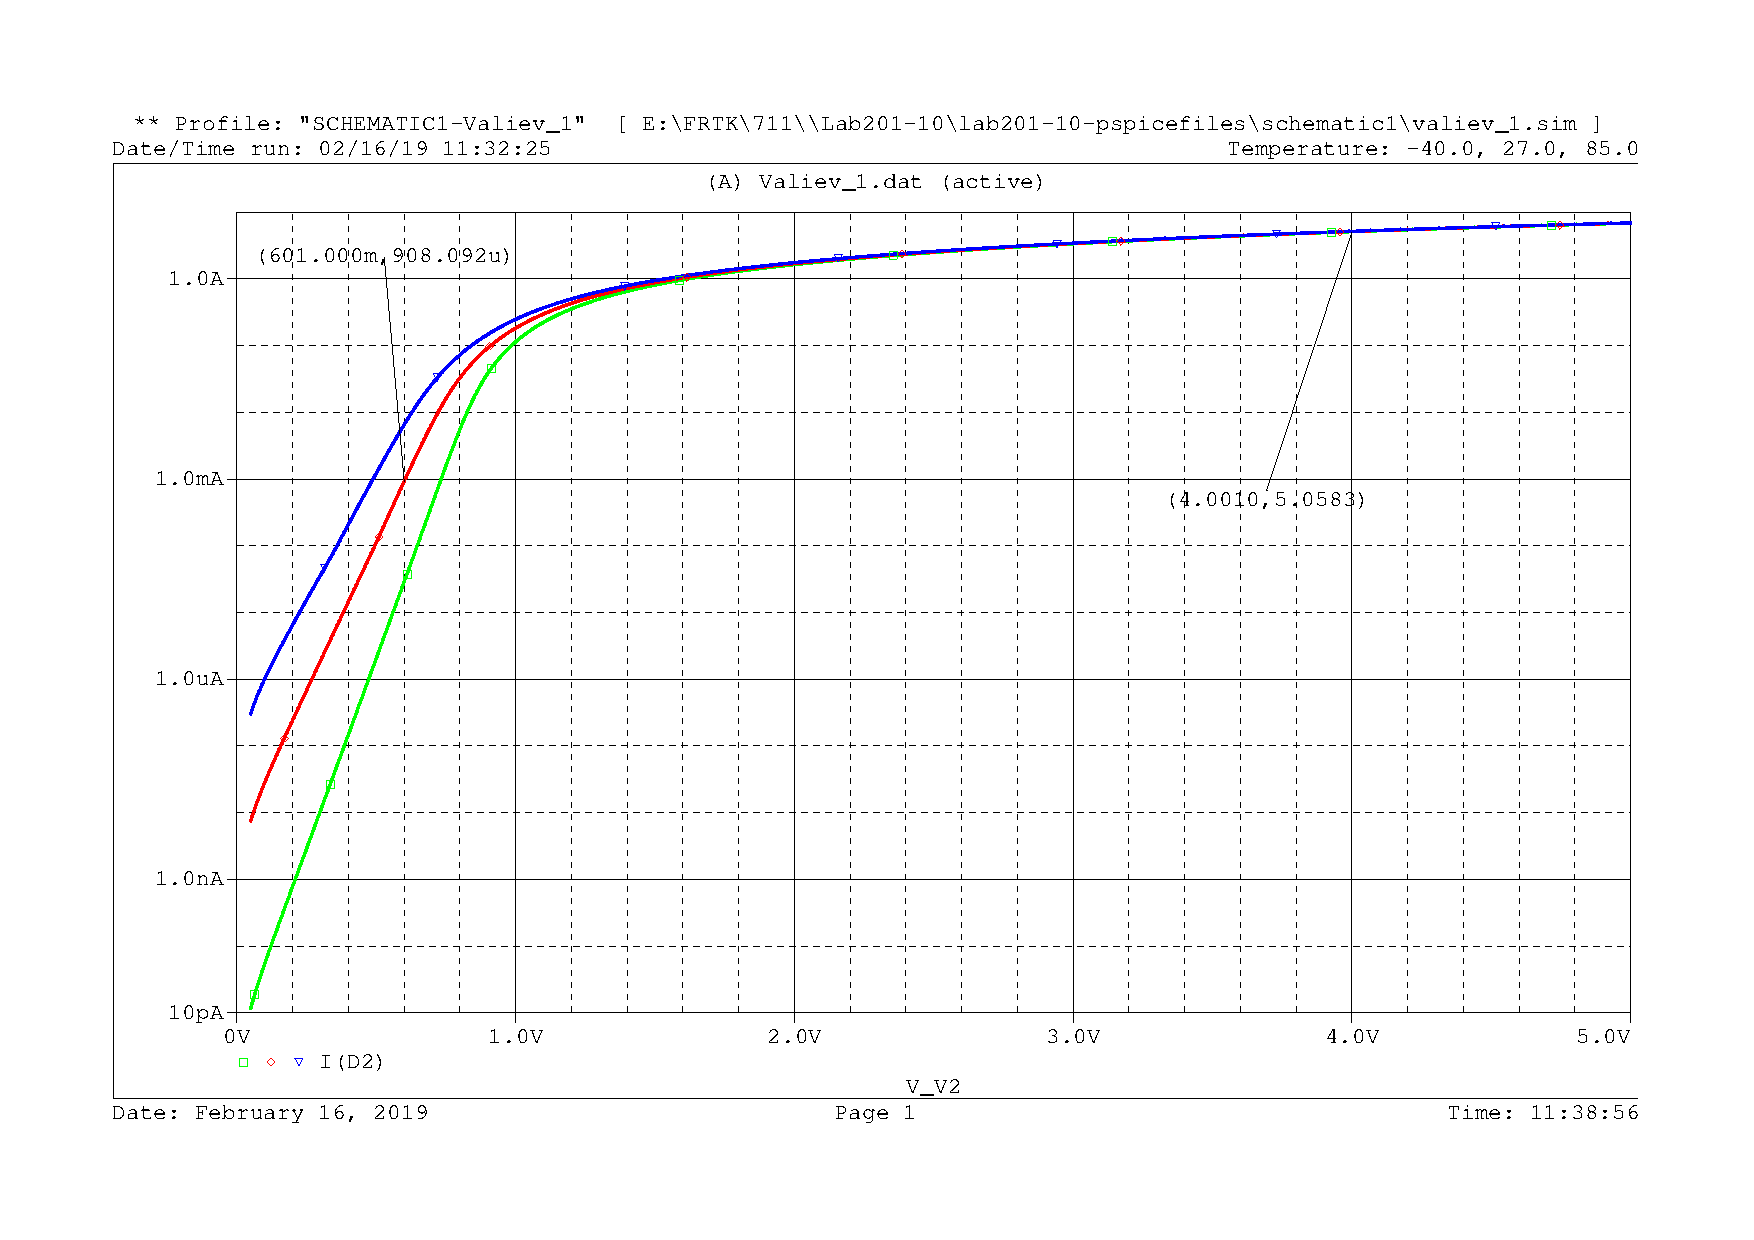
\includegraphics[width = 0.8 \textwidth]{18}
	\caption{ВАХ прямого тока для импульсного ВЧ диода при $ -40\Cd,~27\Cd,~85\Cd $}
	\label{2.1.3.1}
\end{figure}

Для экспоненциальной $ (U_d \approx 0.6V) $ и линейной $ (U_D \approx 4V) $ области ВАХ рассчитаем относительные температурные коэффициенты прямого тока при температуре $ 27 \Cd $.
\begin{equation}\label{eq:Tcoef}
относ.~ТКПТ = \dfrac{абс.~ТКПТ (T)}{I_{пр}(T)} \cdot 100 \left[ \%/\Cd \right]
\end{equation}

\begin{figure}[H]
	\centering
	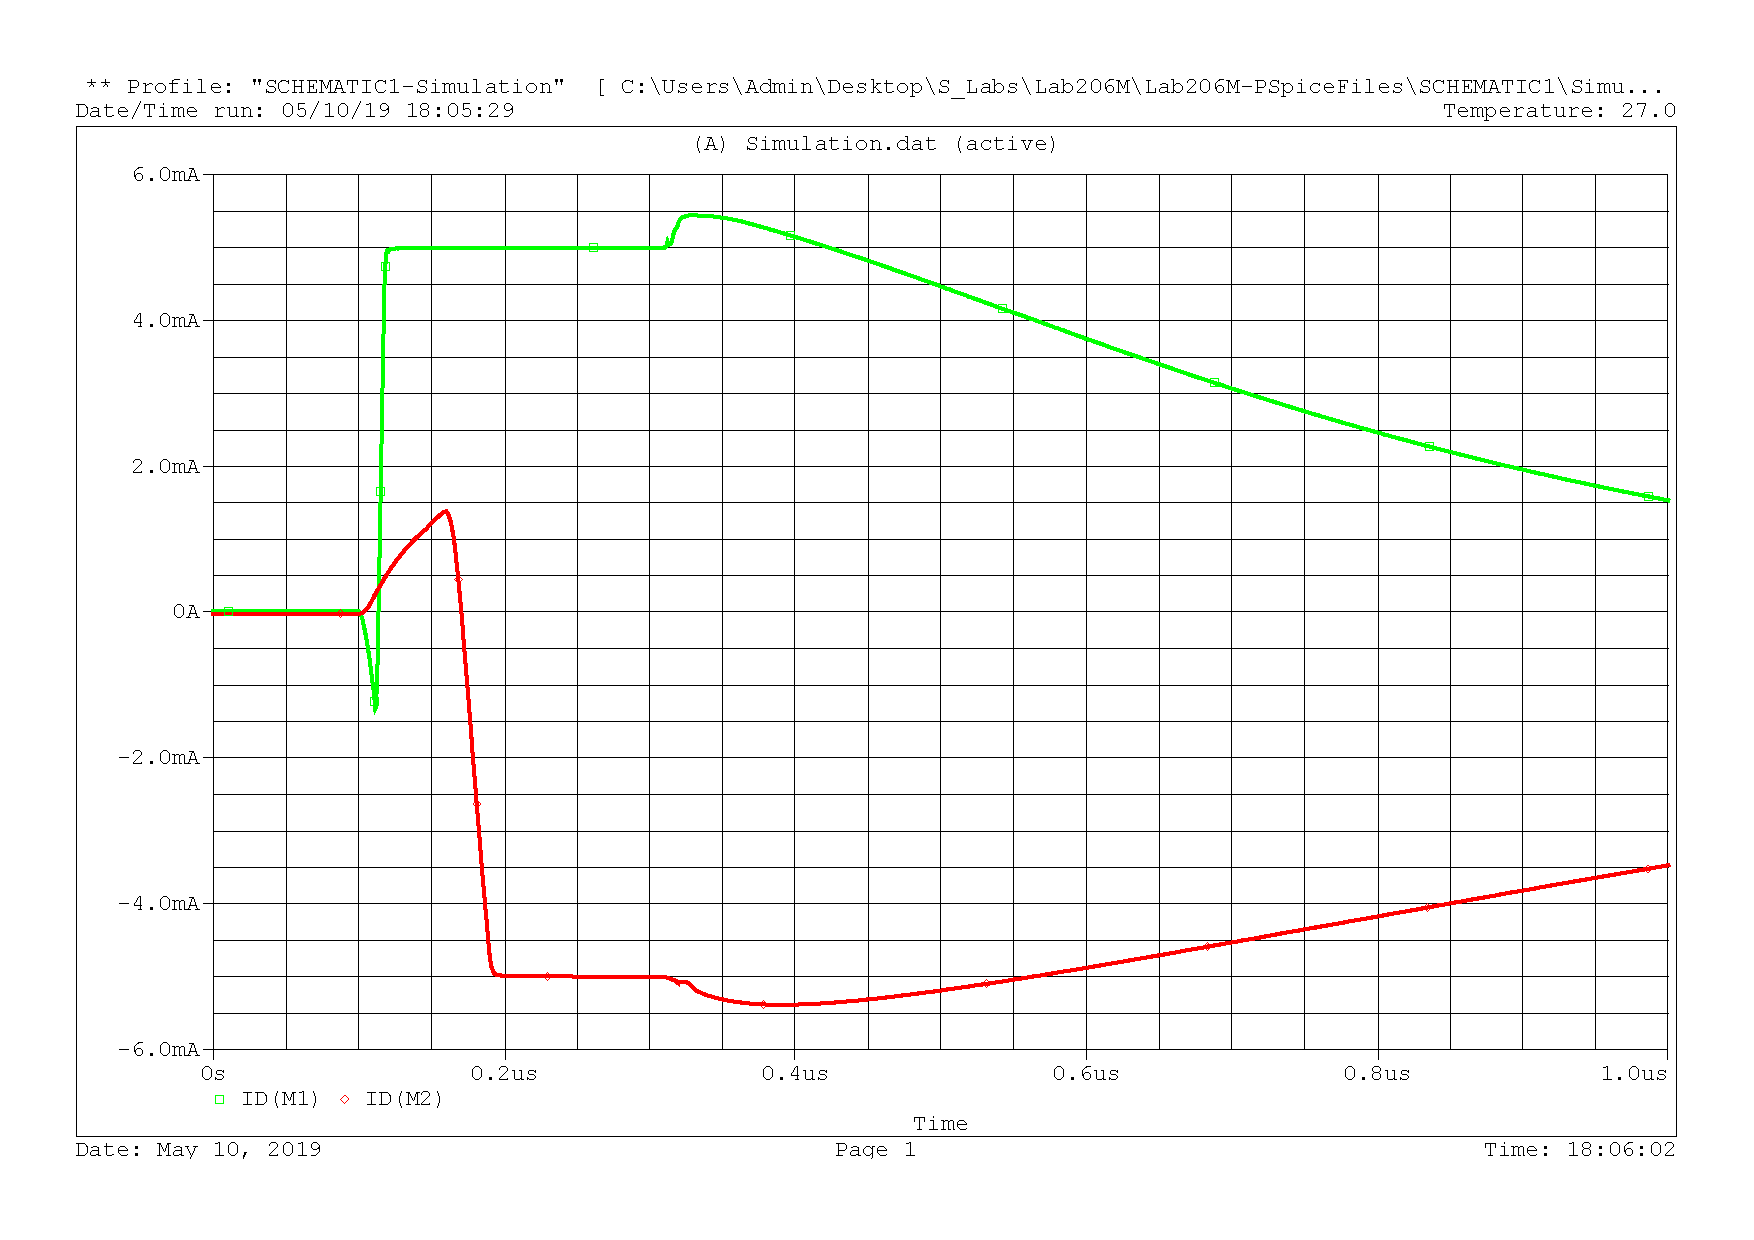
\includegraphics[width = 0.9 \textwidth]{19}
	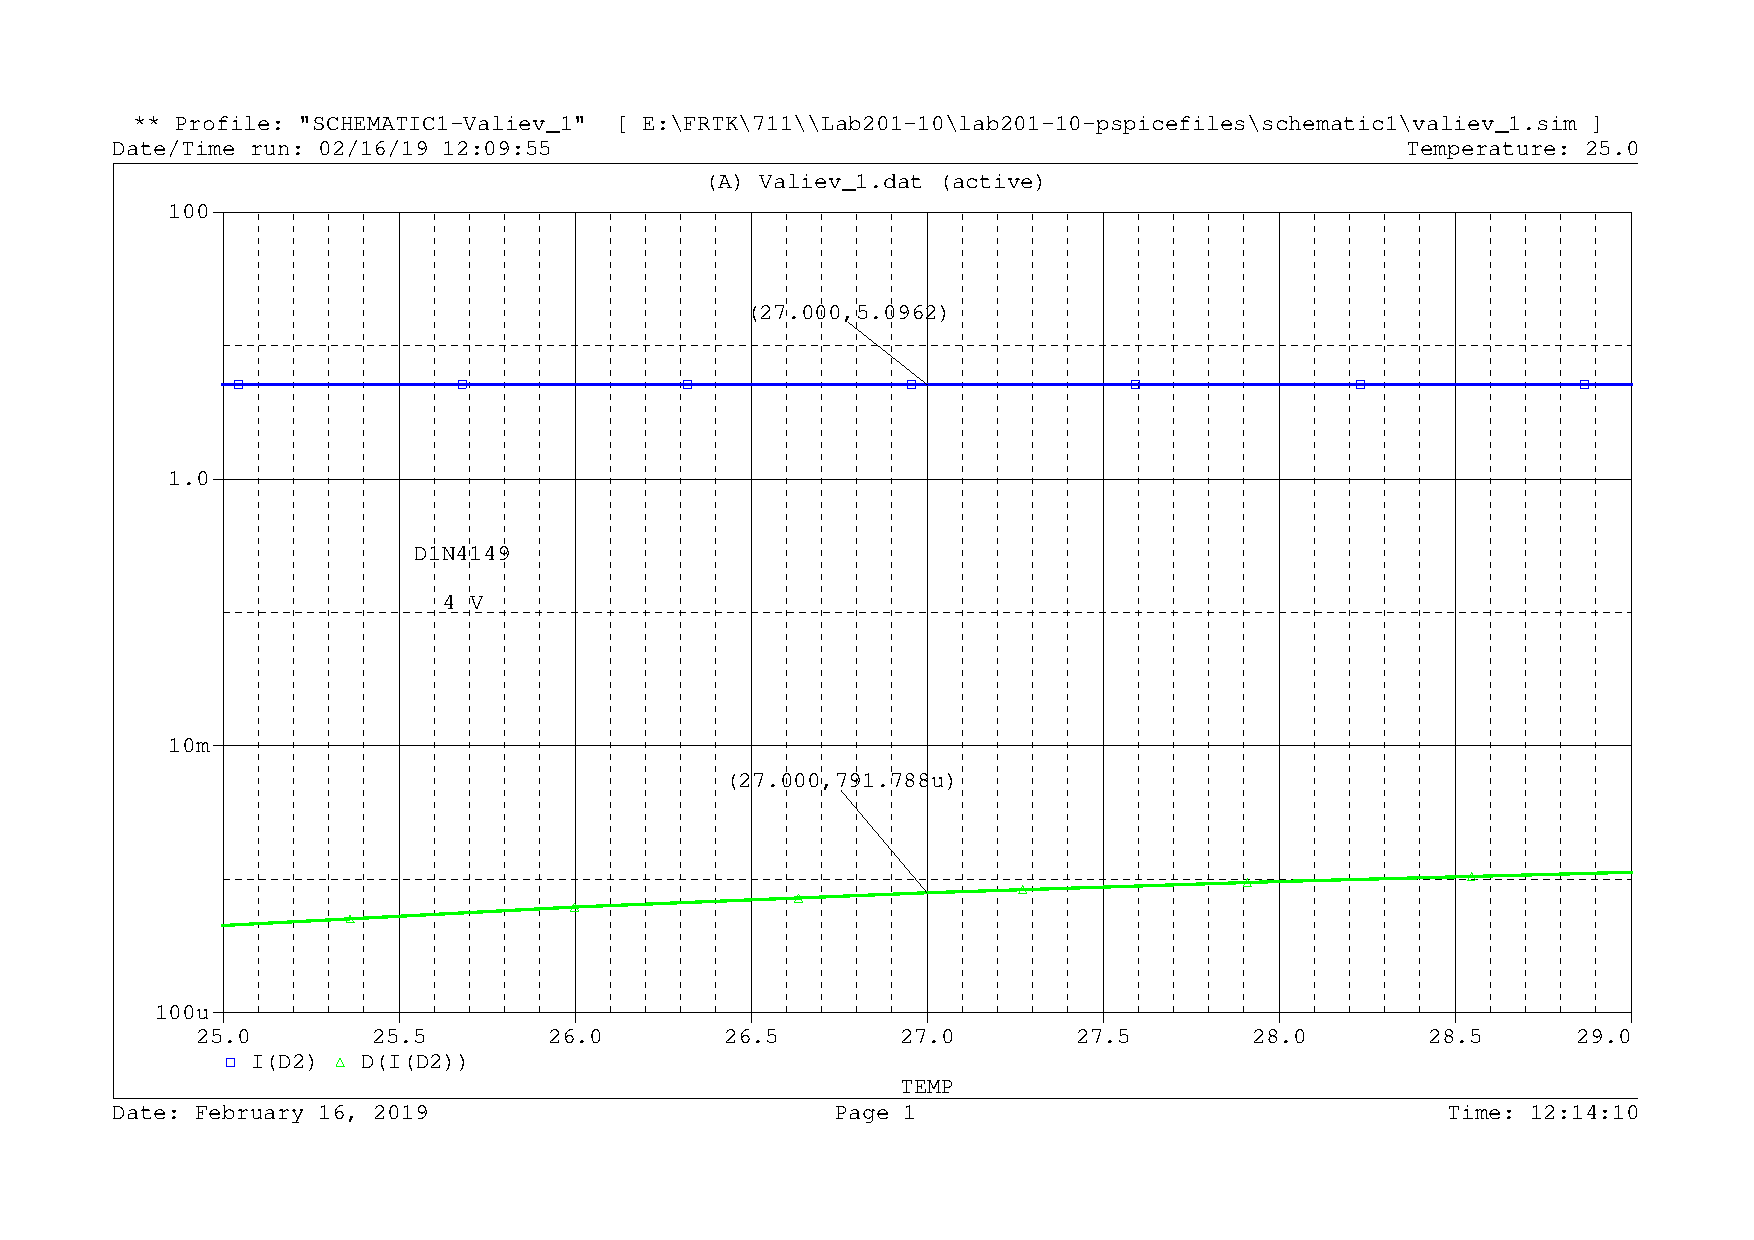
\includegraphics[width = 0.9 \textwidth]{20}
	\caption{Области $ (U_d \approx 0.6V \then ~ ТКПТ \approx 0.1 \%) $ \\
		и $ (U_D \approx 4V) \then ~ ТКПТ \approx 0.4 \%$}
	\label{2.1.3.1_1}
\end{figure}

\newpage

\textbf{{\normalsize 2.1.3.б.}}
Для ВАХ с параметром $ T = 27 \Cd $ в линейном масштабе определим по наклону кривой в области линейности среднее значение омического сопротивления диодной структуры.
\begin{figure}[H]
	\centering
	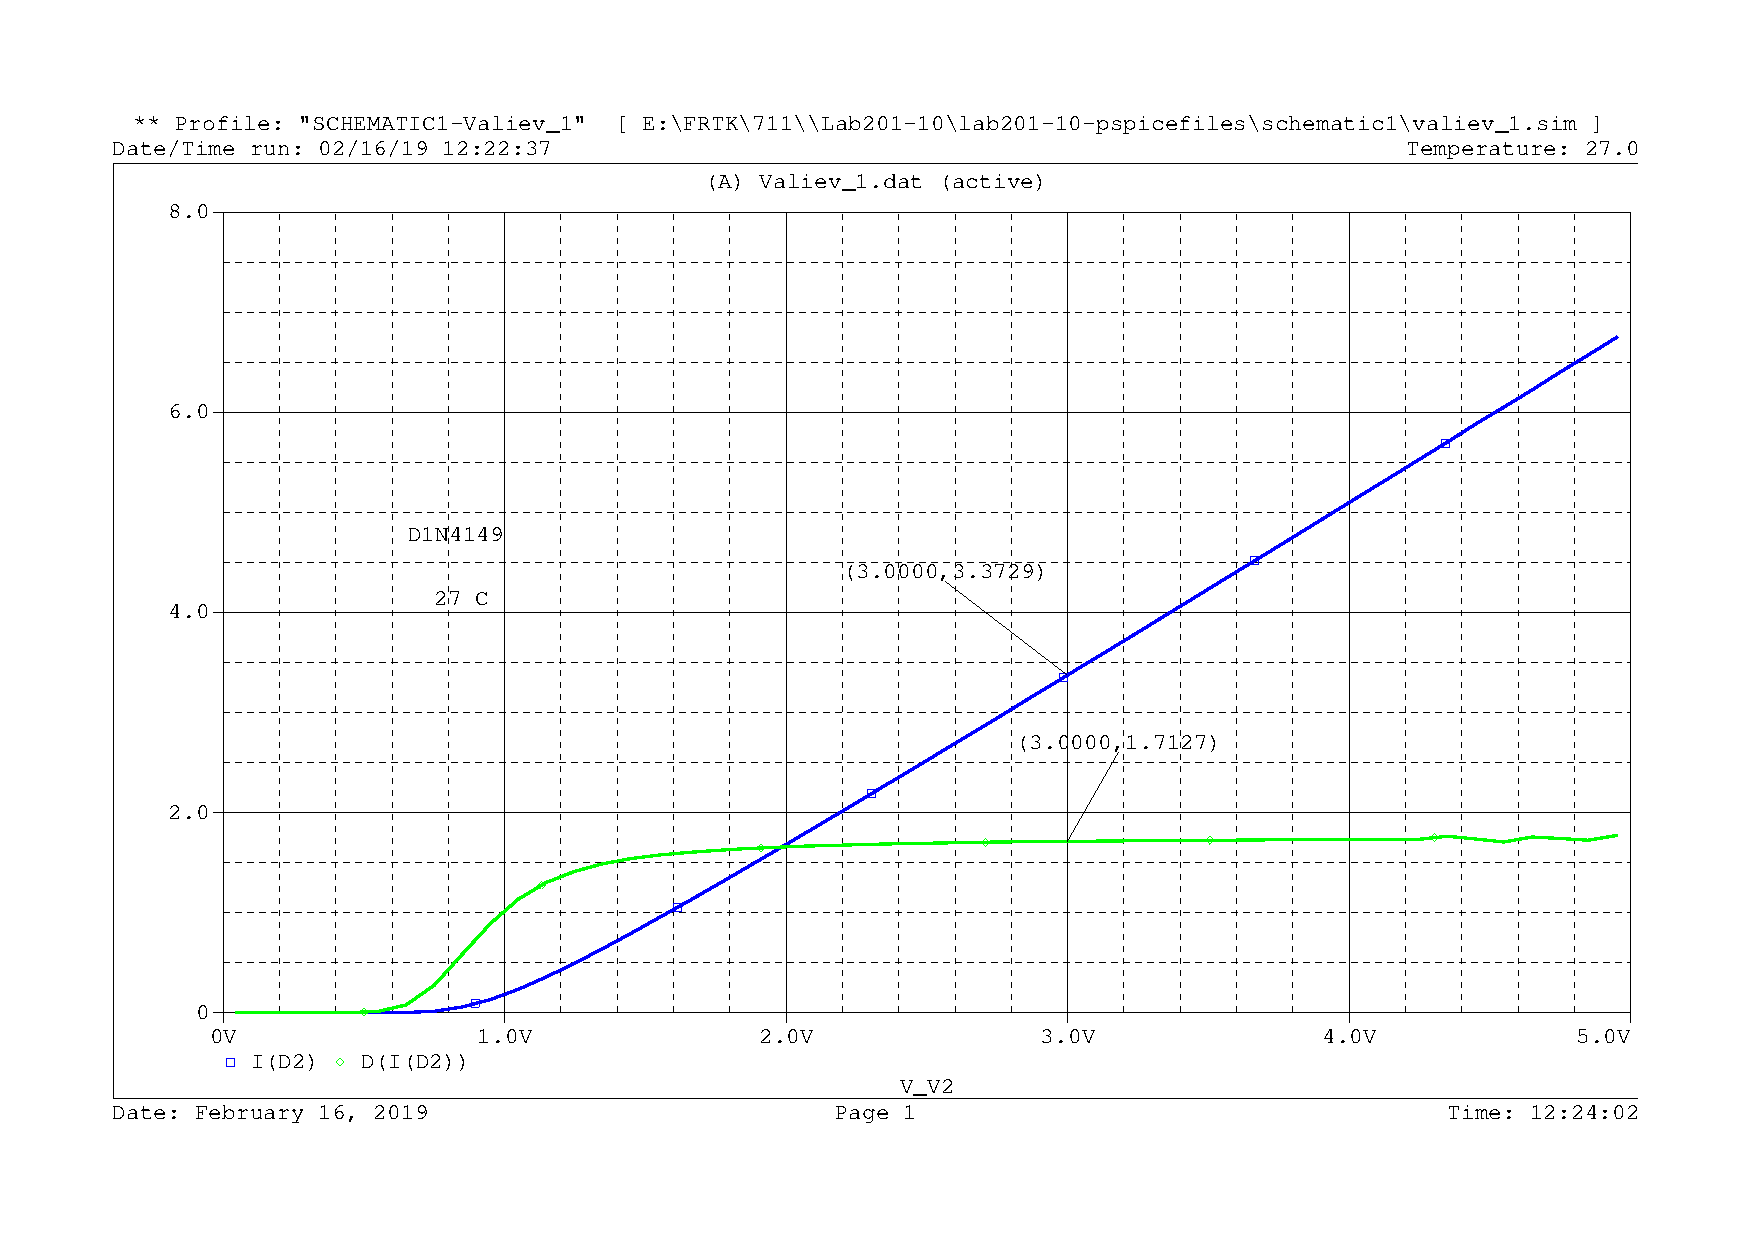
\includegraphics[width = 0.85 \textwidth]{21}
	\caption{Рассматривая $ \dfrac{1}{DIFF} $ приходим к ответу $ .5839 \approx Rs $}
	\label{2.1.3.2}
\end{figure}

\textbf{{\normalsize 2.1.3.в.}}
Найдем также зависимость дифференциальной проводимости.
\begin{figure}[H]
	\centering
	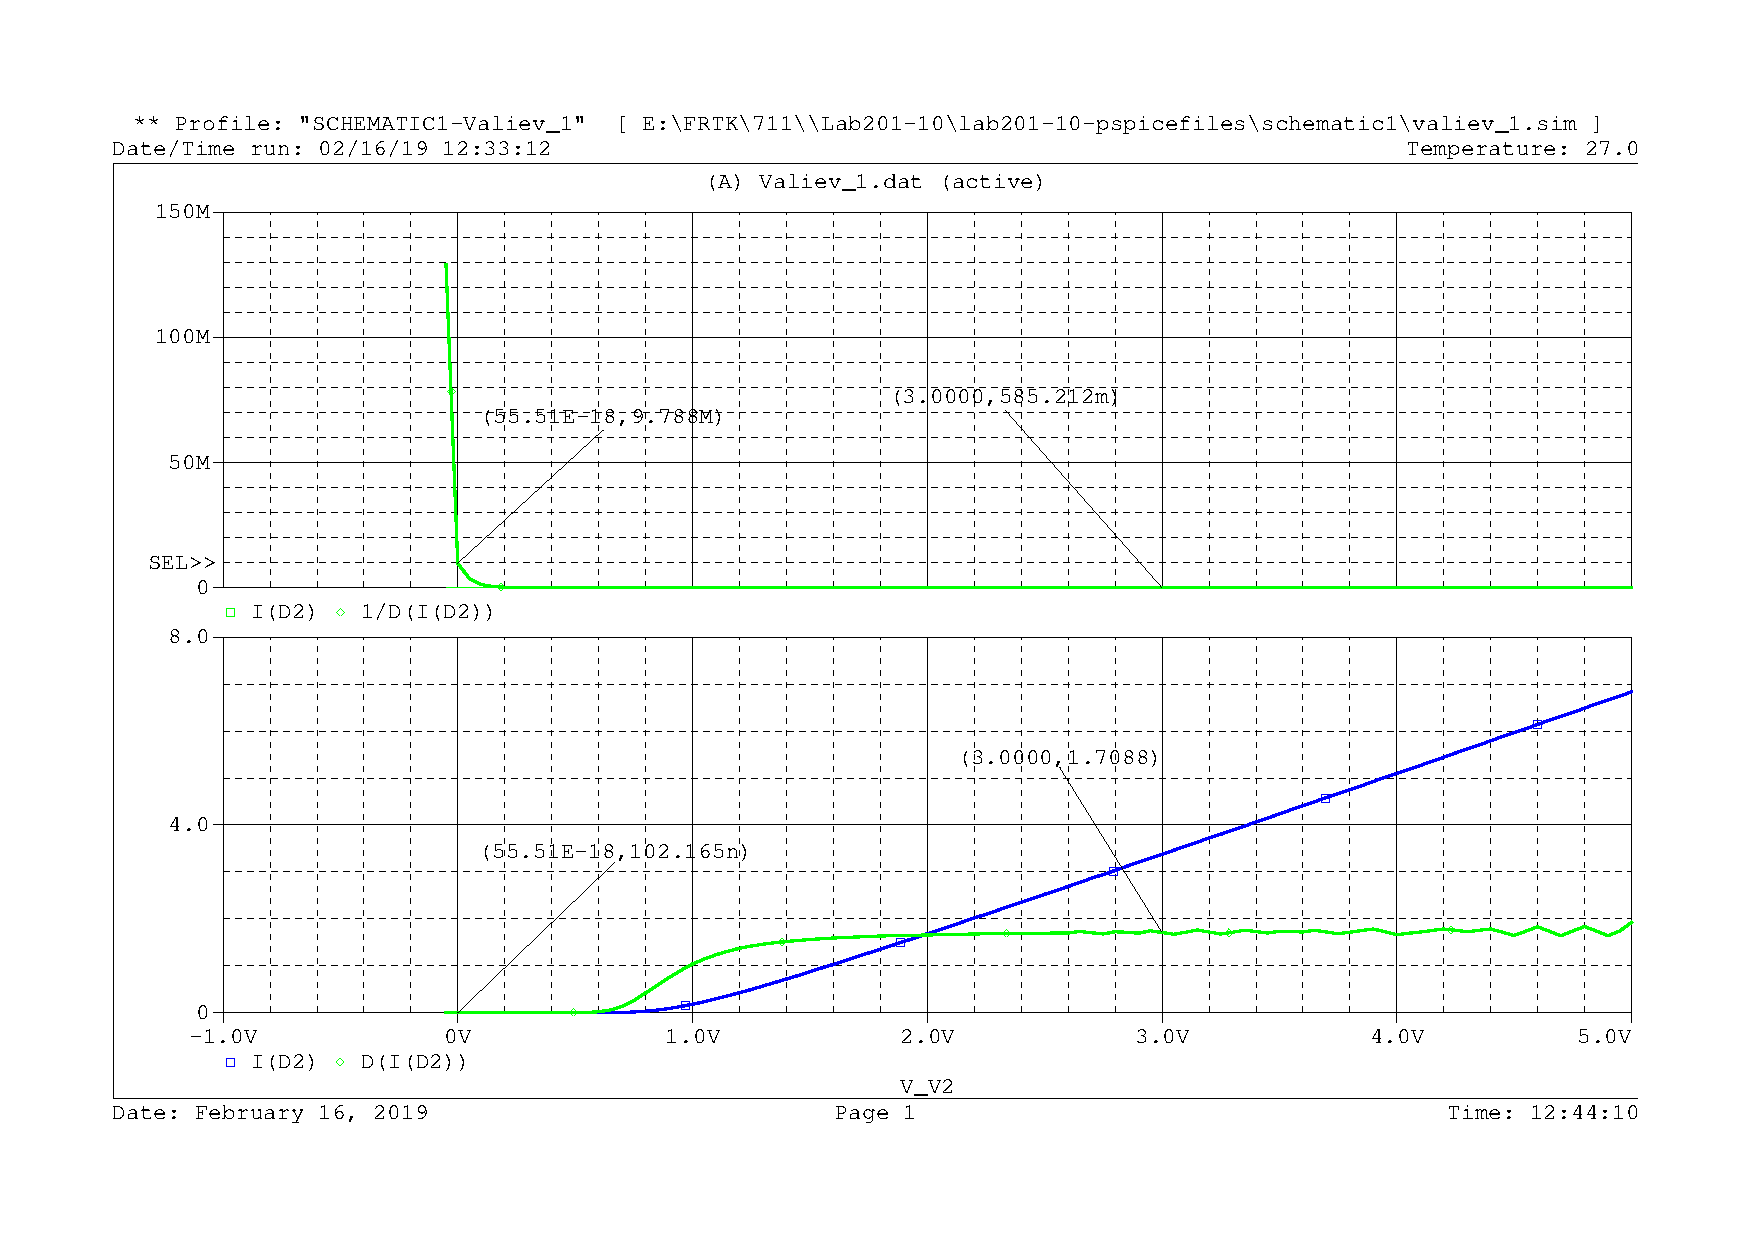
\includegraphics[width = 0.85 \textwidth]{22}
	\caption{Также получаем в линейной области $ .5852 \approx Rs $\\
	При нуле получаем $ r_0 = 9.788M \then \dfrac{U_T}{r_o} = 2.643n \approx I_s $}
	\label{2.1.3.3}
\end{figure}

\textbf{{\normalsize 2.1.3.г.}}
Для ВАХ с параметром $ T = 27 \Cd $ в линейном масштабе получим в области экспоненциальной зависимости коэффициент неидеальности при $ I_{xx} = Is ~ или ~ Isr $.
\begin{equation}\label{eq:ideal}
m = \left. \dfrac{U}{U_T} \right/ \ln \left( \dfrac{I + Is}{Is} \right) \approx \left( \dfrac{U}{U_T} \right) \left/ \right. \ln \left( \dfrac{I}{I_{xx}} \right)
\end{equation}

\begin{figure}[H]
	\centering
	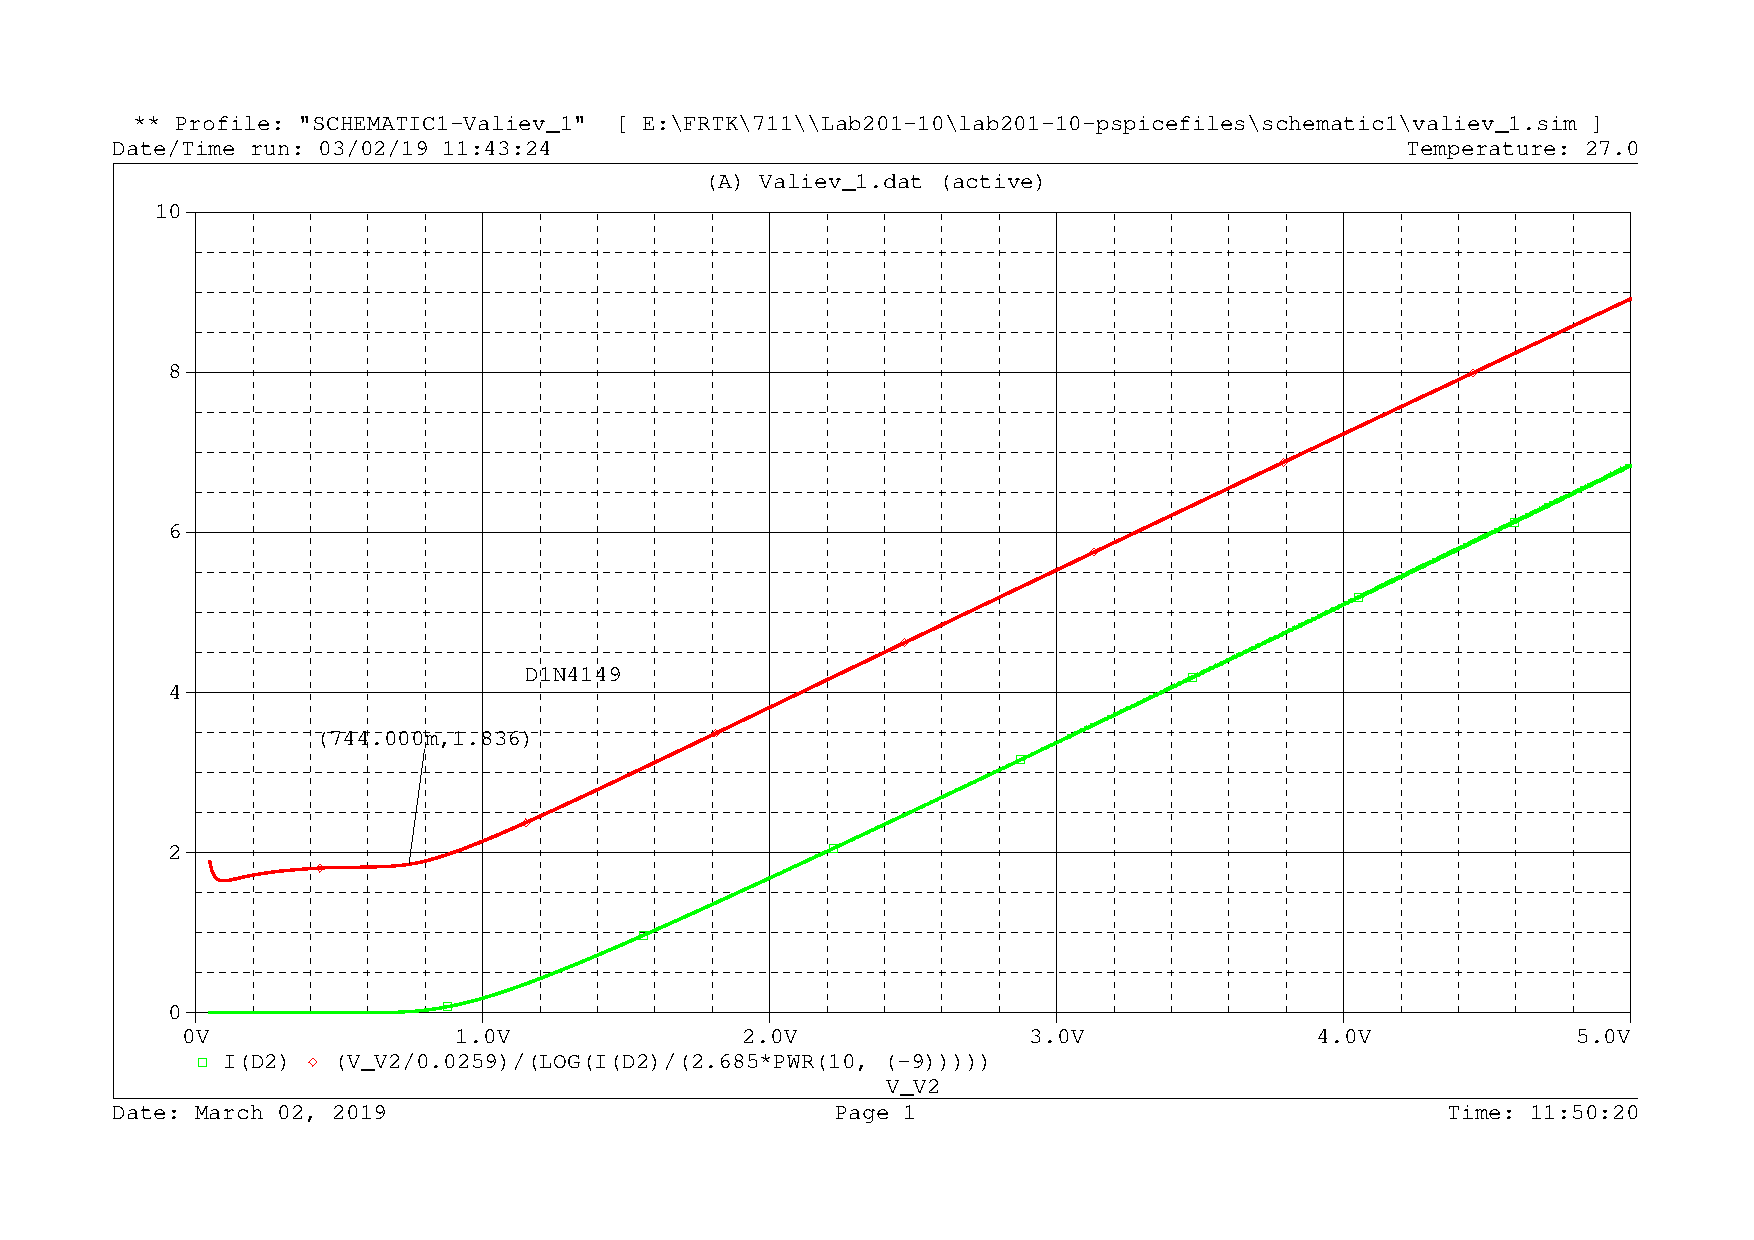
\includegraphics[width = 0.85 \textwidth]{23}
	\caption{Коэффициент неидеальности $ (Is) = 1.836 \approx N $: совпадает с паспортом}
	\label{2.1.3.4_1}
\end{figure}

\begin{figure}[H]
	\centering
	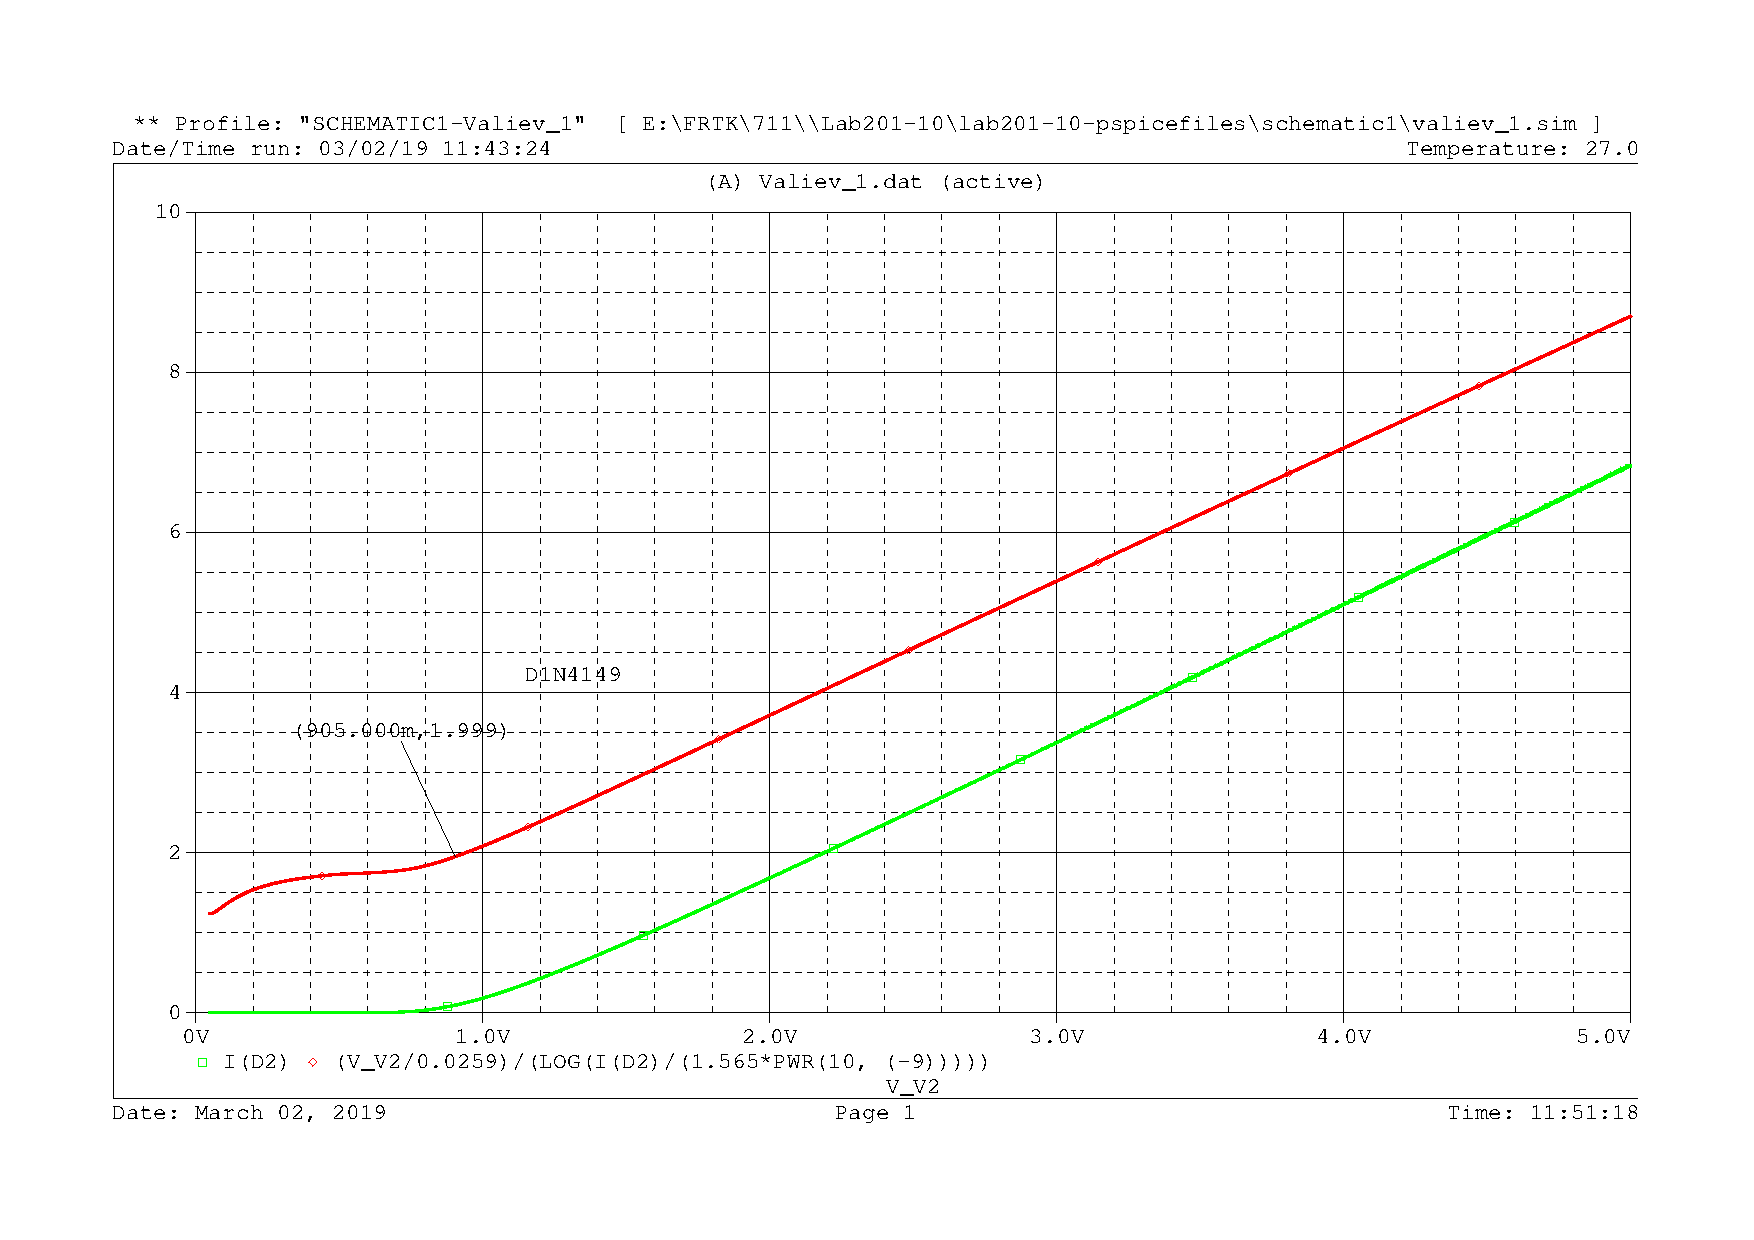
\includegraphics[width = 0.85 \textwidth]{24}
	\caption{Коэффициент неидеальности $ (Isr) = 1.999 \approx Nr $: совпадает с паспортом}
	\label{2.1.3.4_2}
\end{figure}

\newpage

\subsubsection*{ВАХ стабилитрона $ I_{стб} = f(U, T = const) $}

\textbf{{\normalsize 2.1.4.}}
Получим зависимости тока стабилитрона от напряжения в диапазоне\\
от $ -(U_{st} + \Delta U) $ до $ +0.3V $ при $ -40 \Cd, 27 \Cd, 85 \Cd $. Также рассмотрим это в малой окрестности напряжения стабилизации.
\begin{figure}[H]
	\centering
	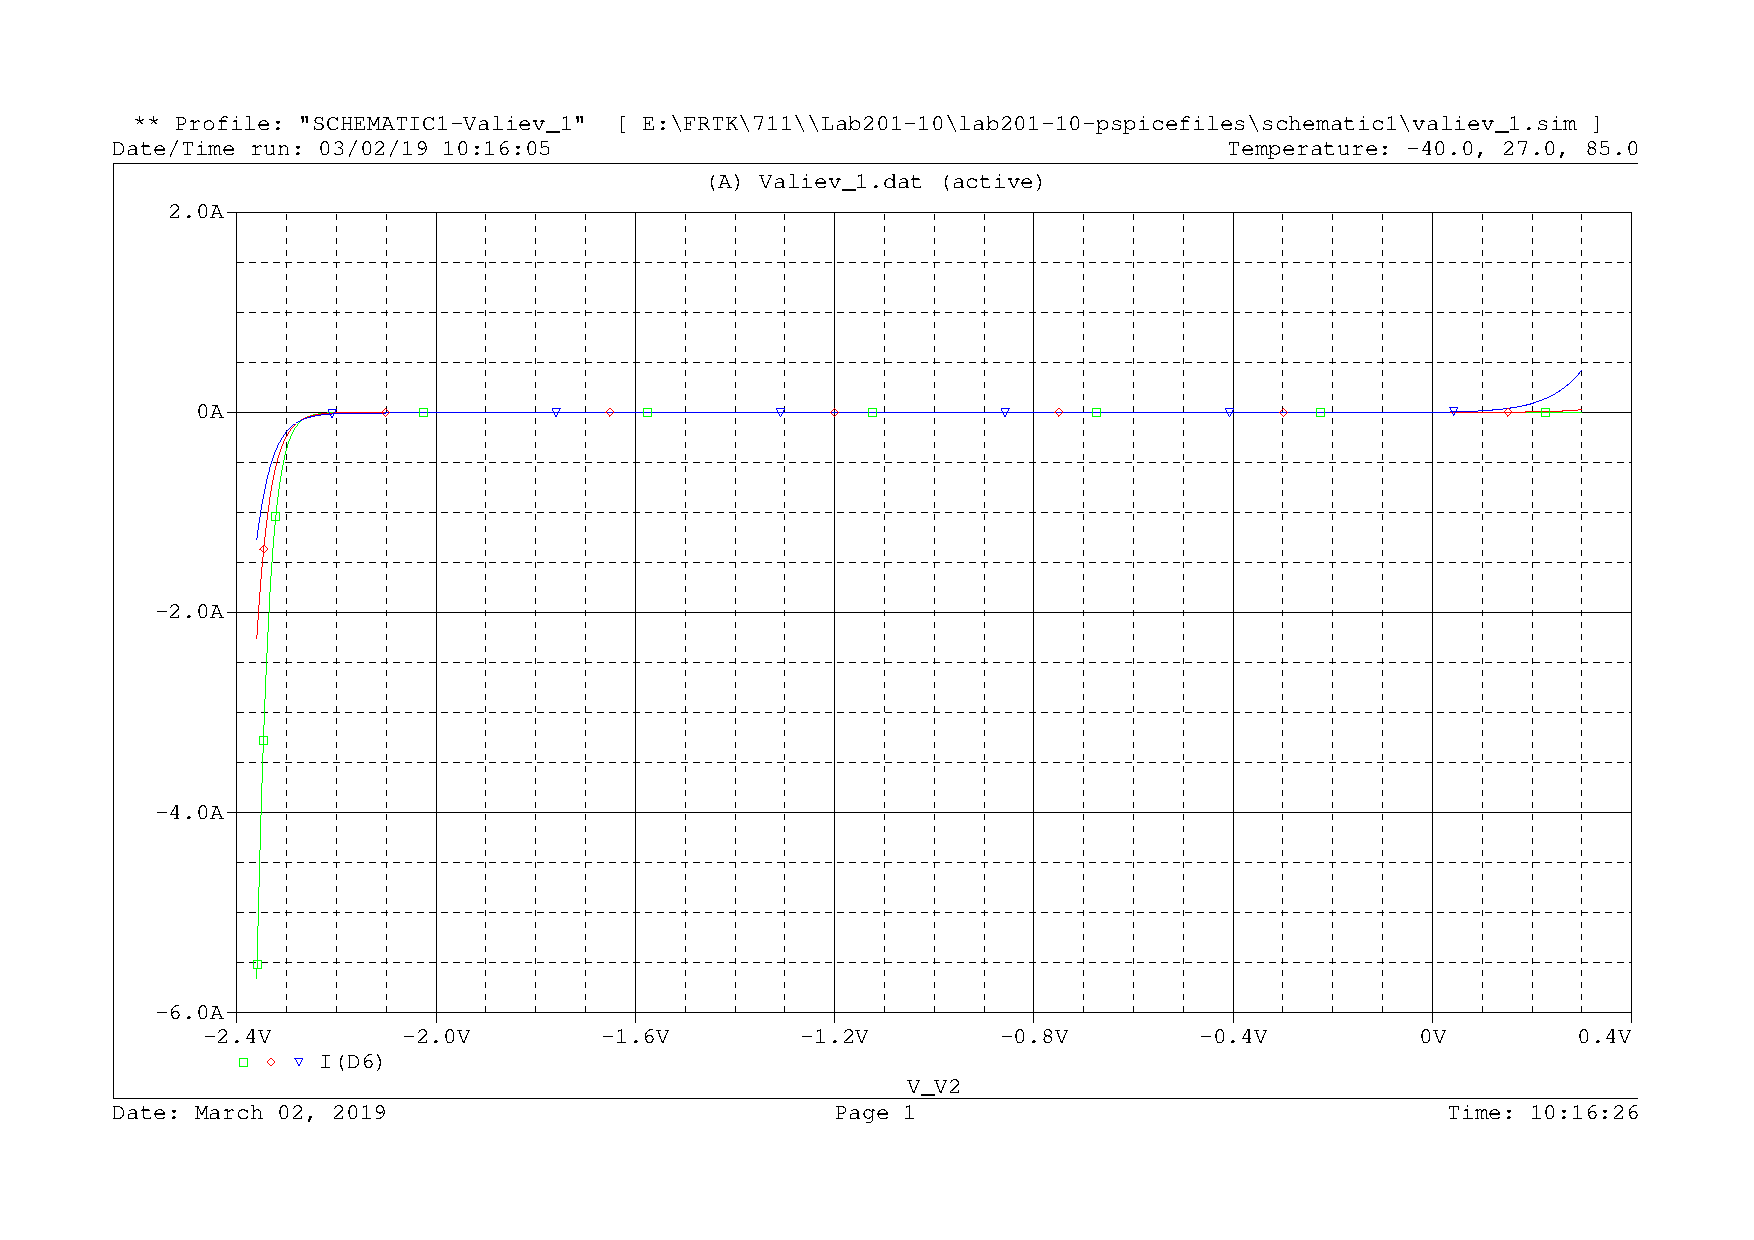
\includegraphics[width = 0.9 \textwidth]{26}
	\caption{ВАХ стабилитрона}
	\label{2.1.4_1}
\end{figure}

\begin{figure}[H]
	\centering
	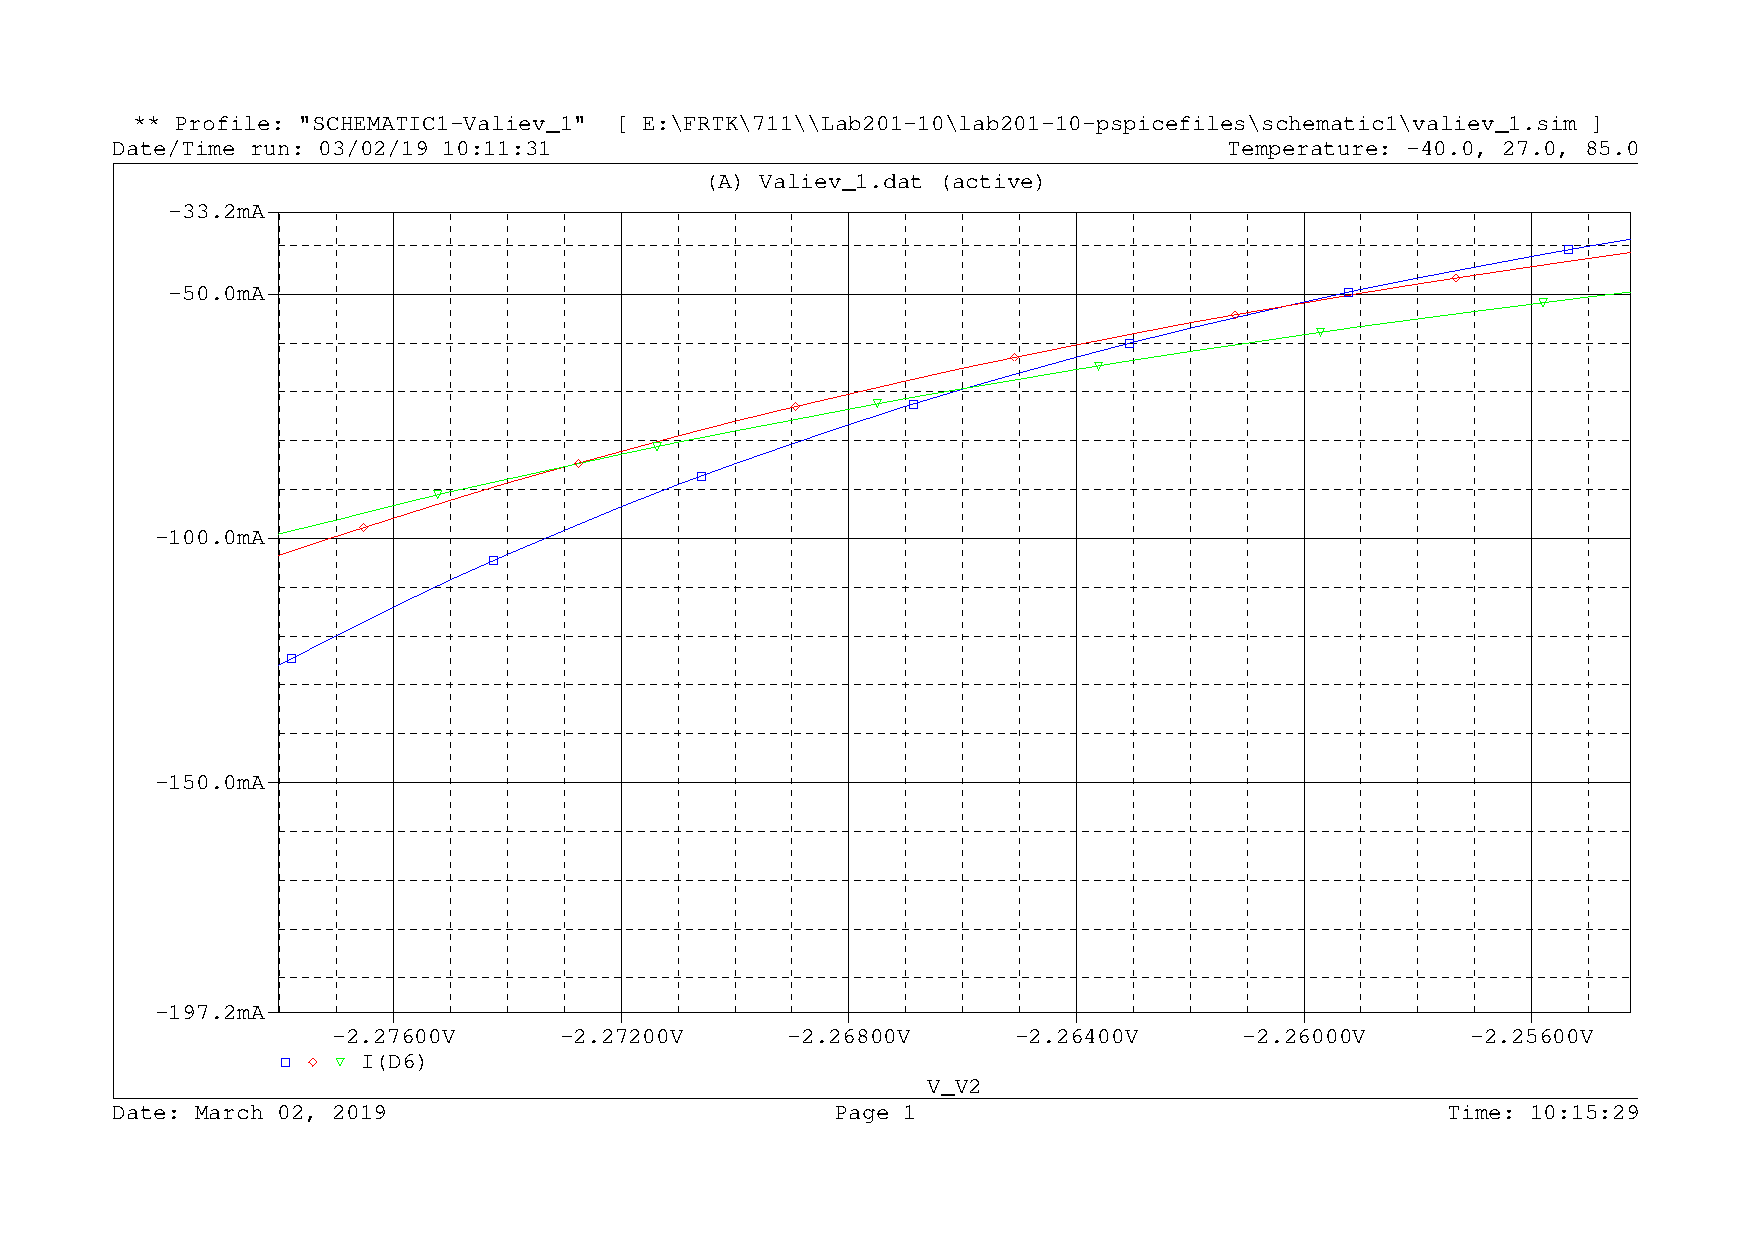
\includegraphics[width = 0.9 \textwidth]{25}
	\caption{ВАХ стабилитрона вблизи напряжения стабилизации}
	\label{2.1.4_2}
\end{figure}

\subsubsection*{Обратная ветвь ВАХ реального диода}

\textbf{{\normalsize 2.1.5.}}
Отсоединим стабилитрон от источника и получим зависимости токов диодов от напряжения в диапазоне от $ -(30-60)V $ до $ +0.05V $ при $ T = 27 \Cd $.
\begin{figure}[H]
	\centering
	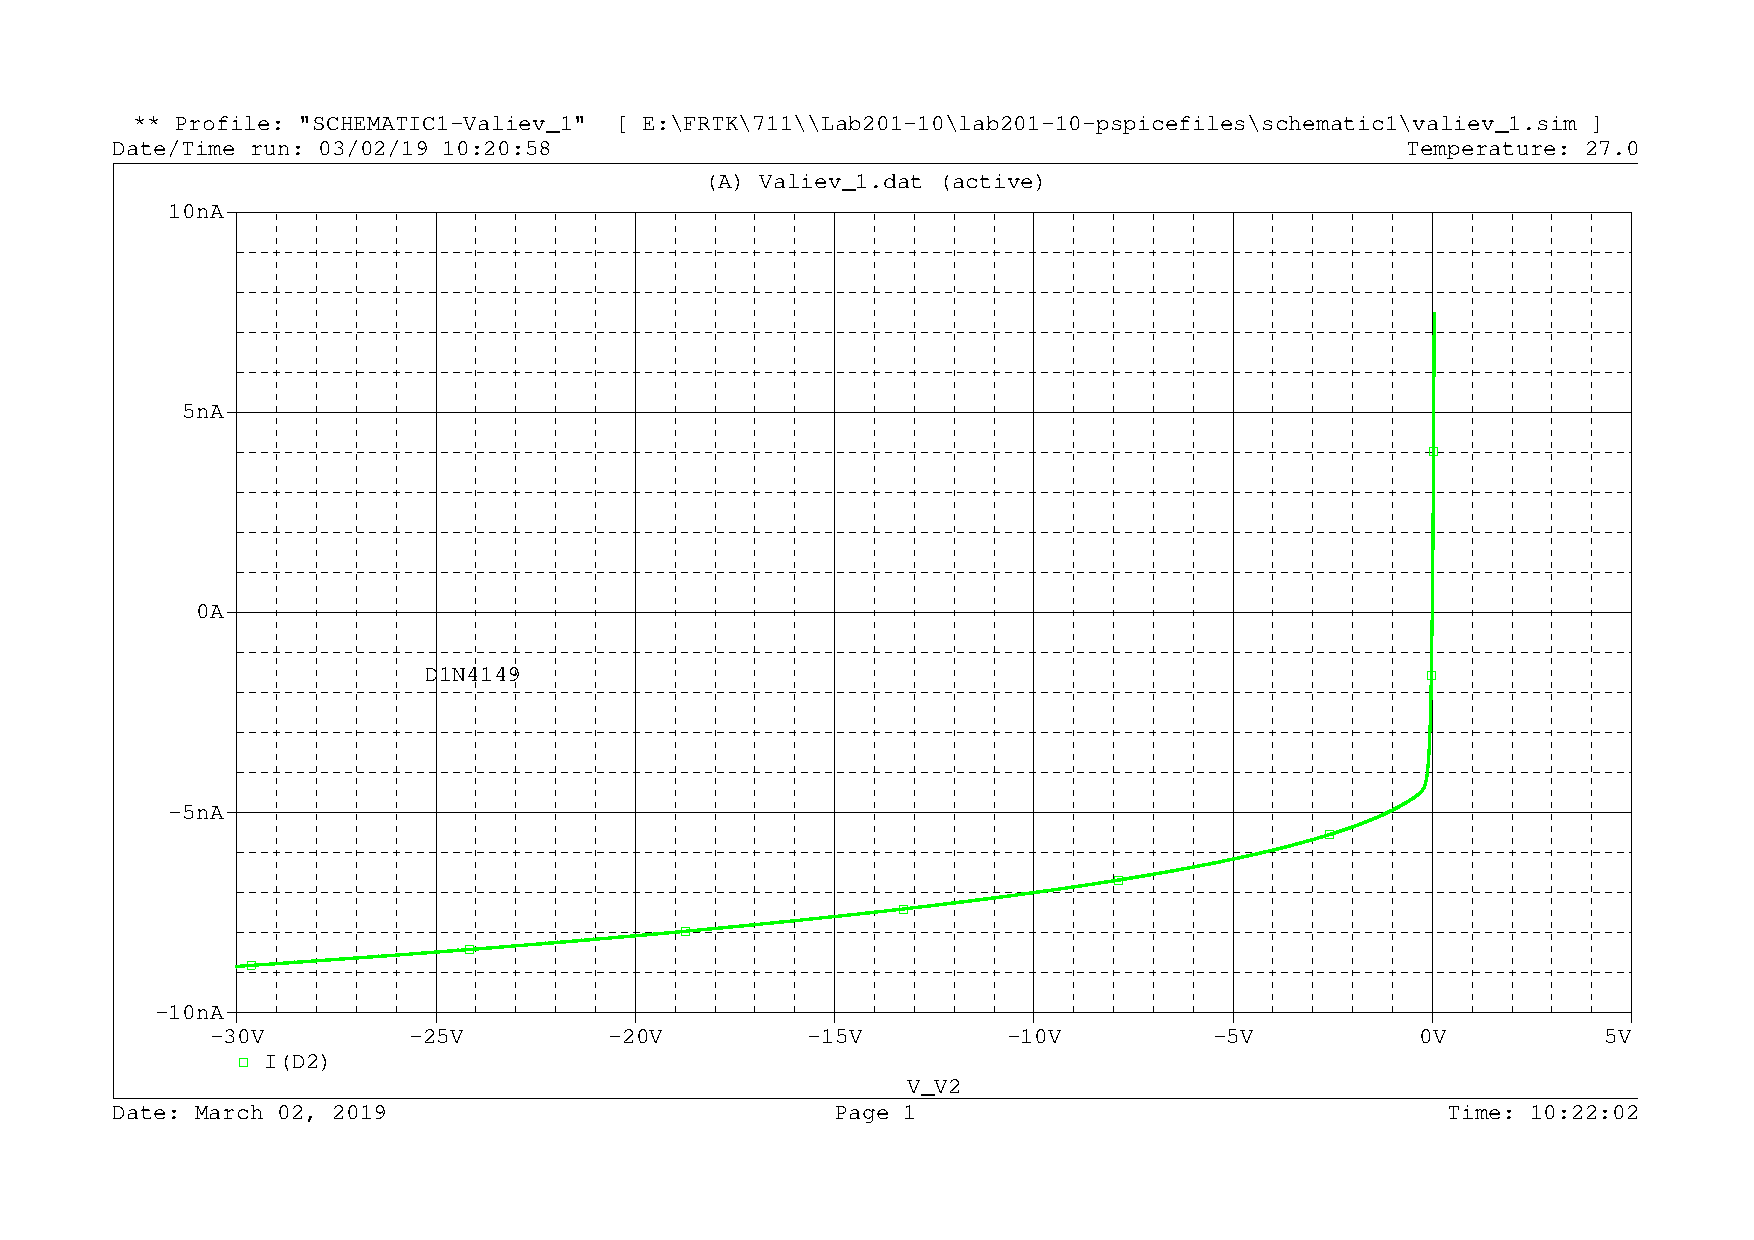
\includegraphics[width = 0.9 \textwidth]{27}
	\caption{D1N4149}
	\label{2.1.5_1}
\end{figure}

\begin{figure}[H]
	\centering
	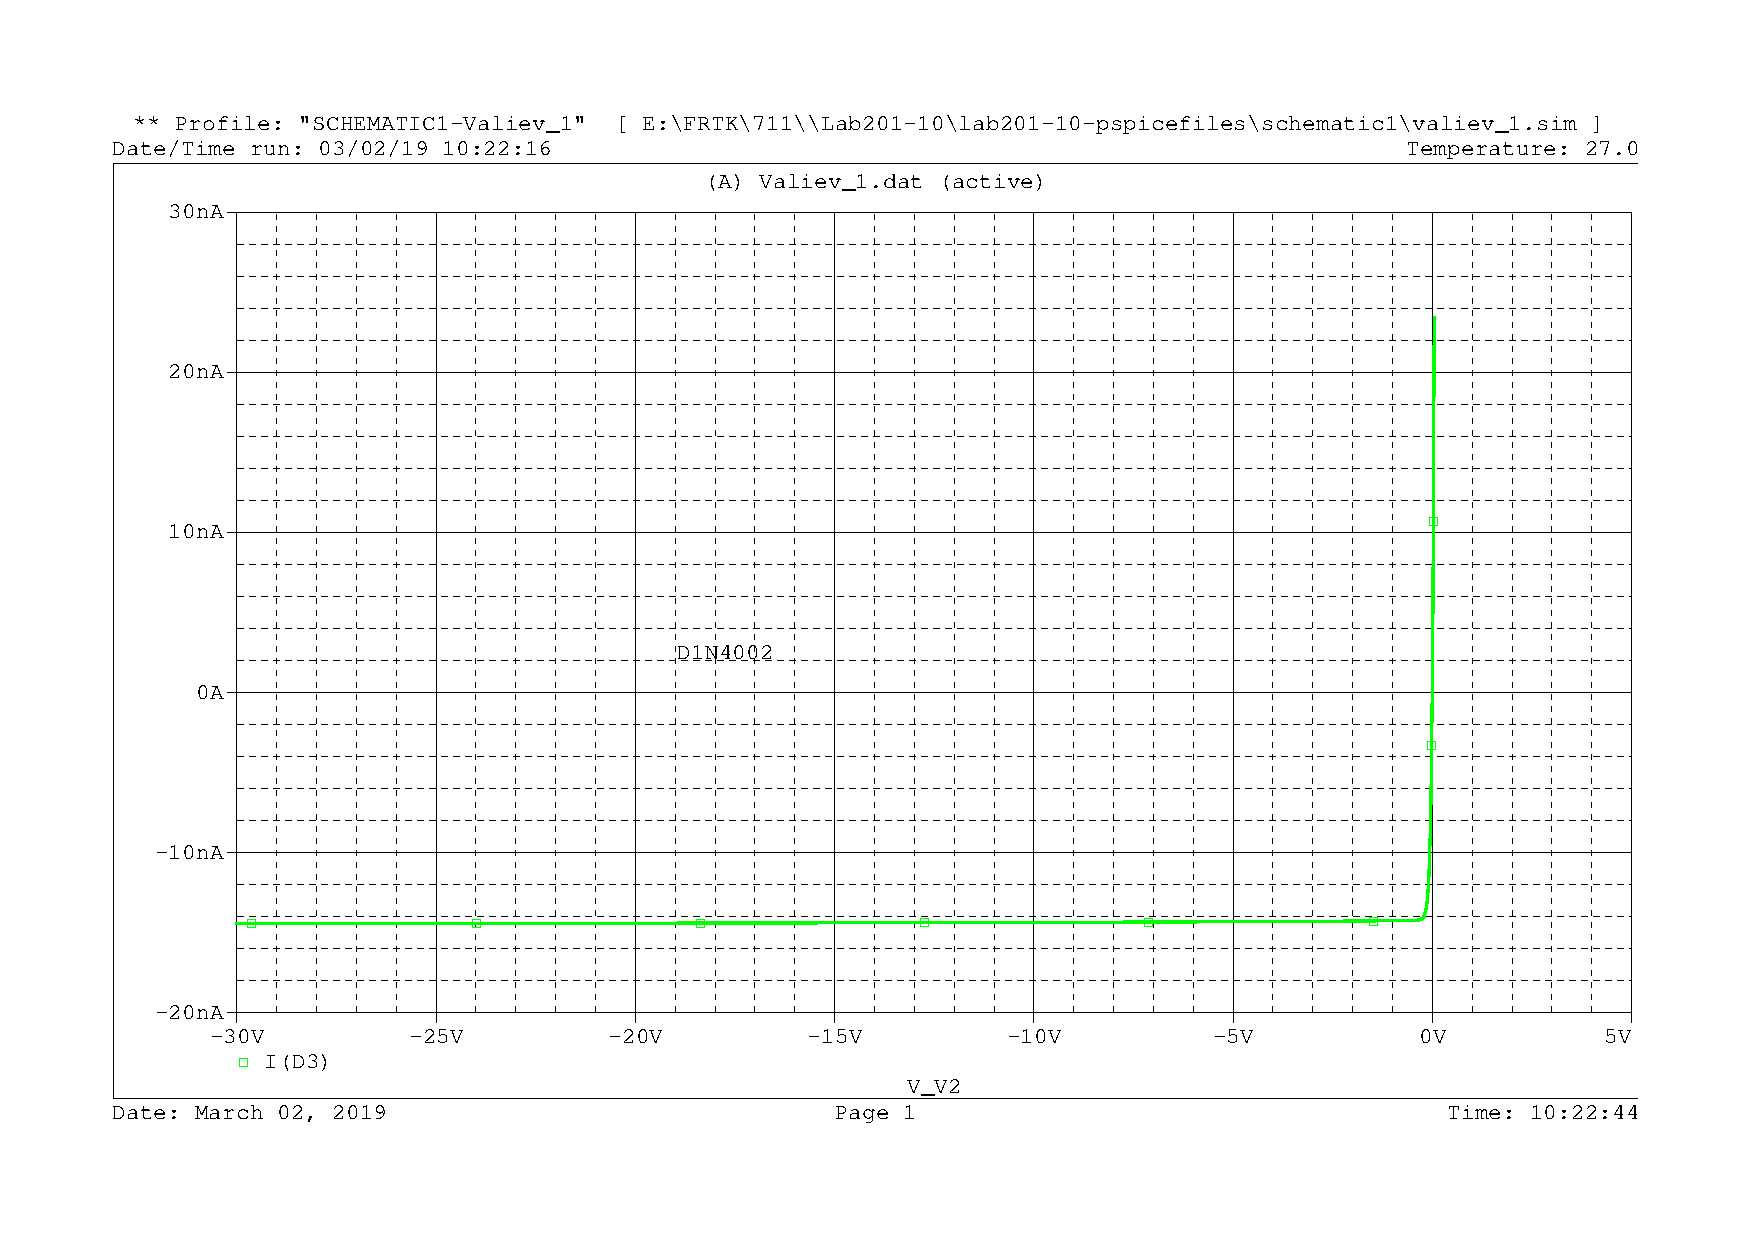
\includegraphics[width = 0.9 \textwidth]{28}
	\caption{D1N4002}
	\label{2.1.5_2}
\end{figure}

\begin{figure}[H]
	\centering
	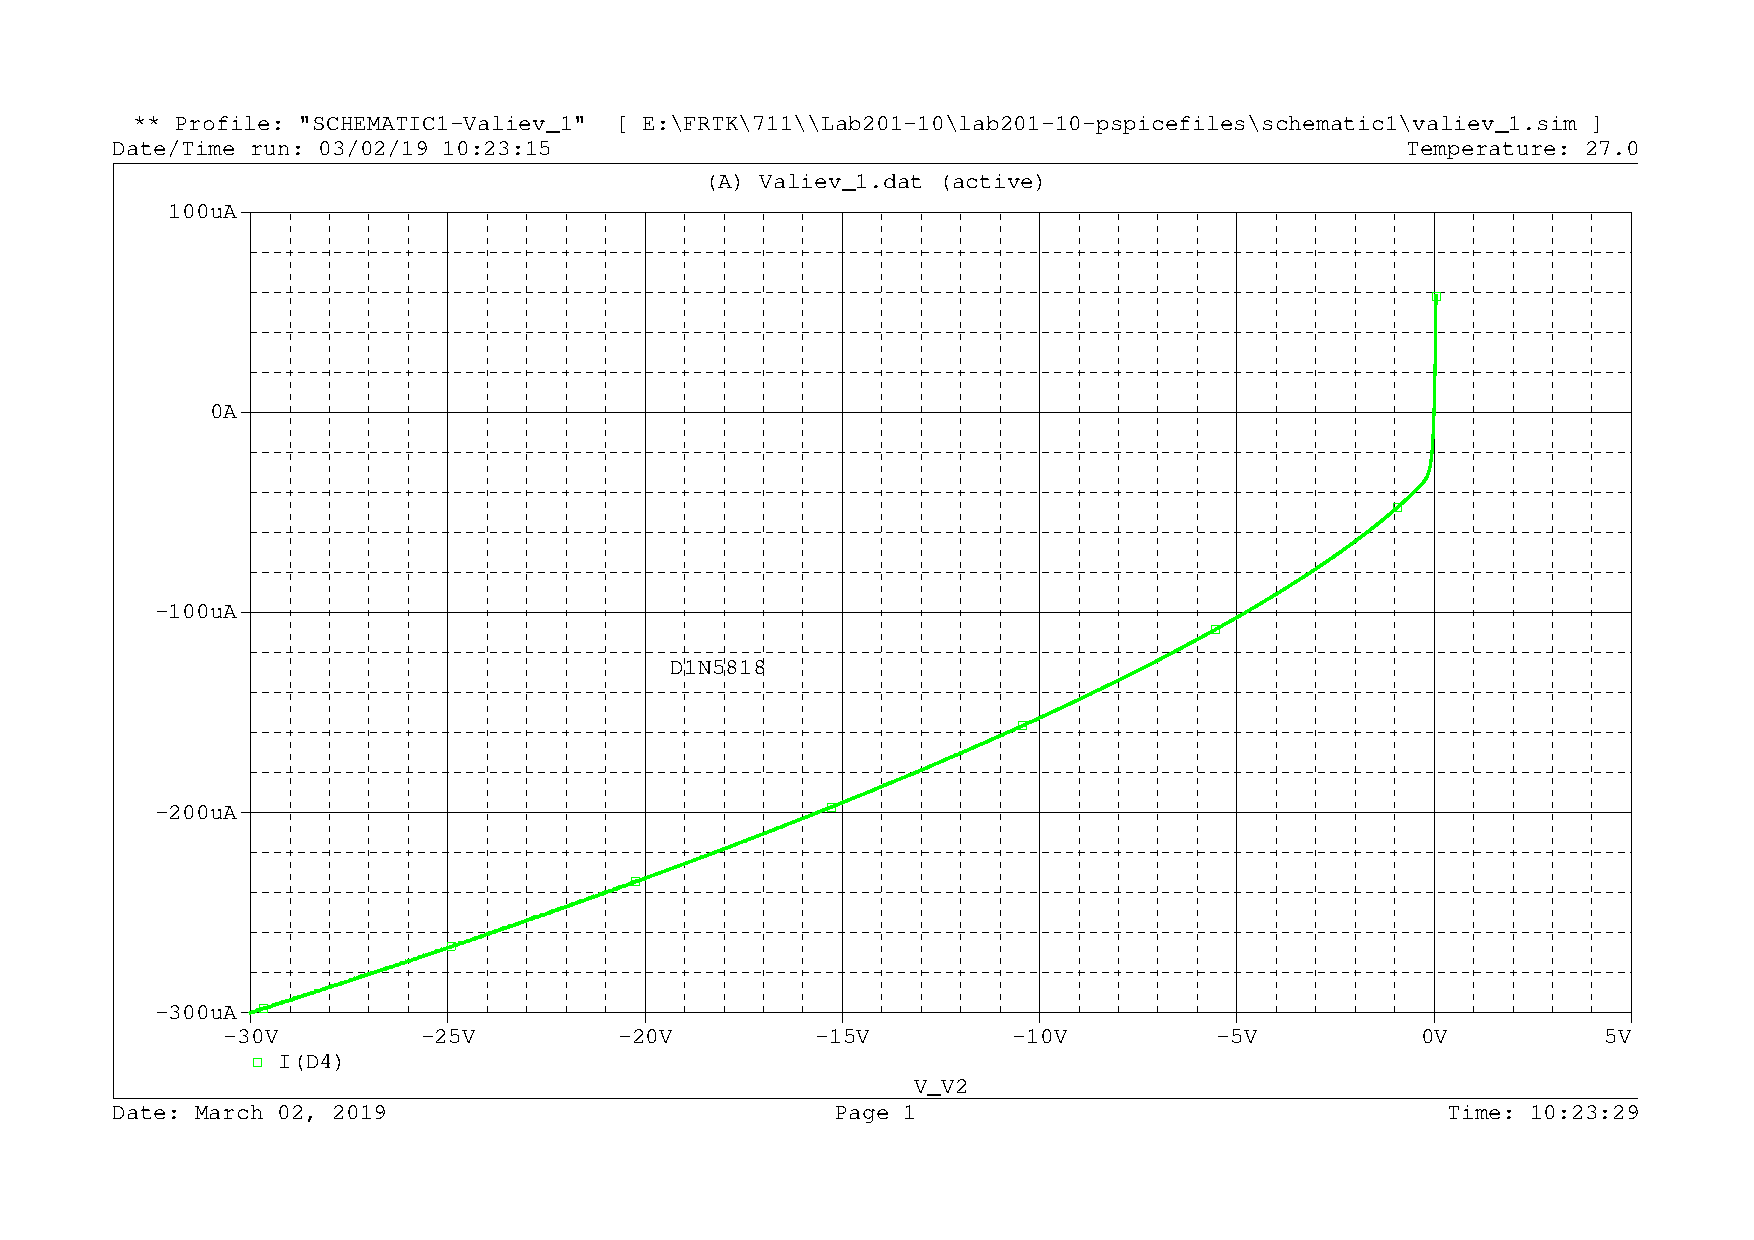
\includegraphics[width = \textwidth]{29}
	\caption{D1N5818}
	\label{2.1.5_3}
\end{figure}

\begin{figure}[H]
	\centering
	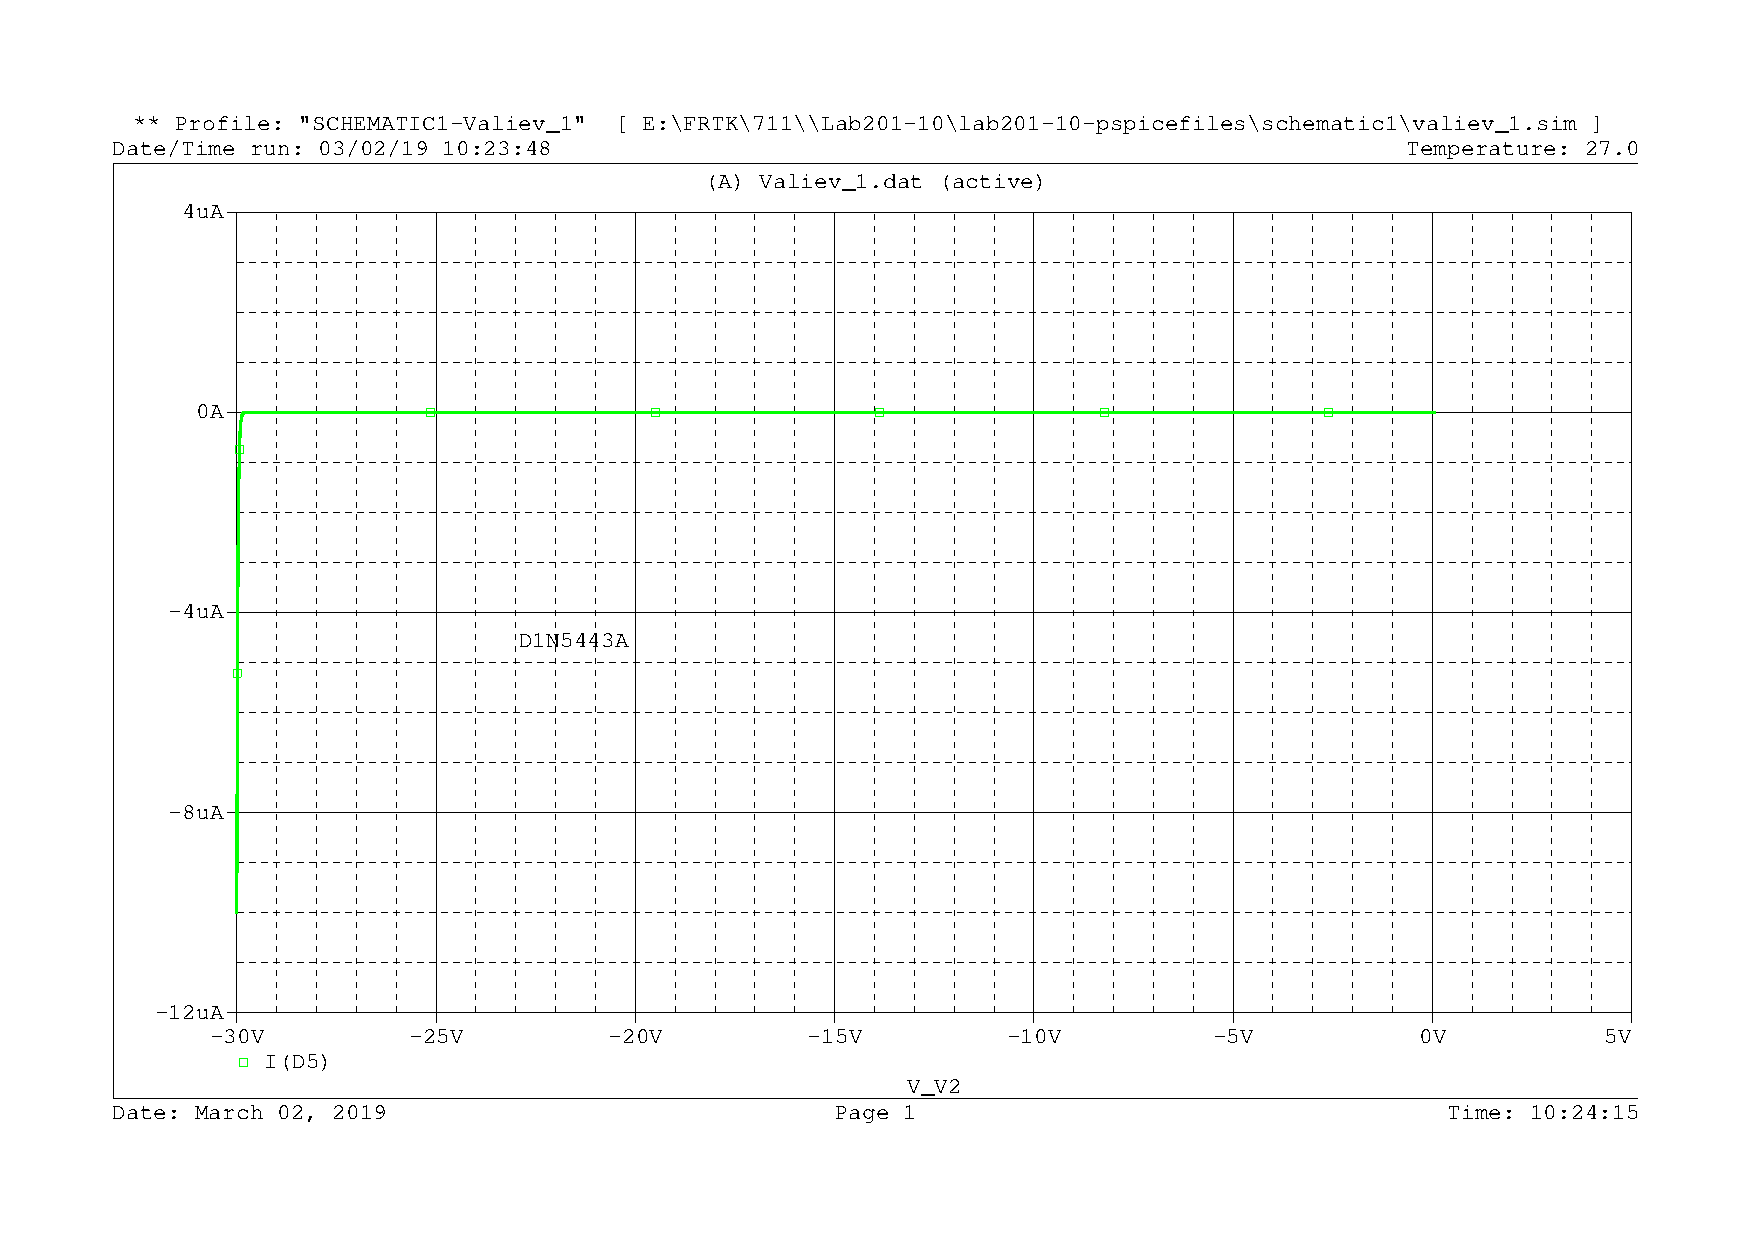
\includegraphics[width = \textwidth]{30}
	\caption{D1N5443A}
	\label{2.1.5_4}
\end{figure}



\subsection*{2.2. Температурные характеристики}

\textbf{{\normalsize 2.2.1.}}
Установим напряжение $ V = 0.6V $. Получим зависимости прямого тока от температуры в диапазоне от $ -50 \Cd $ до $ +100 \Cd $.
\begin{figure}[H]
	\centering
	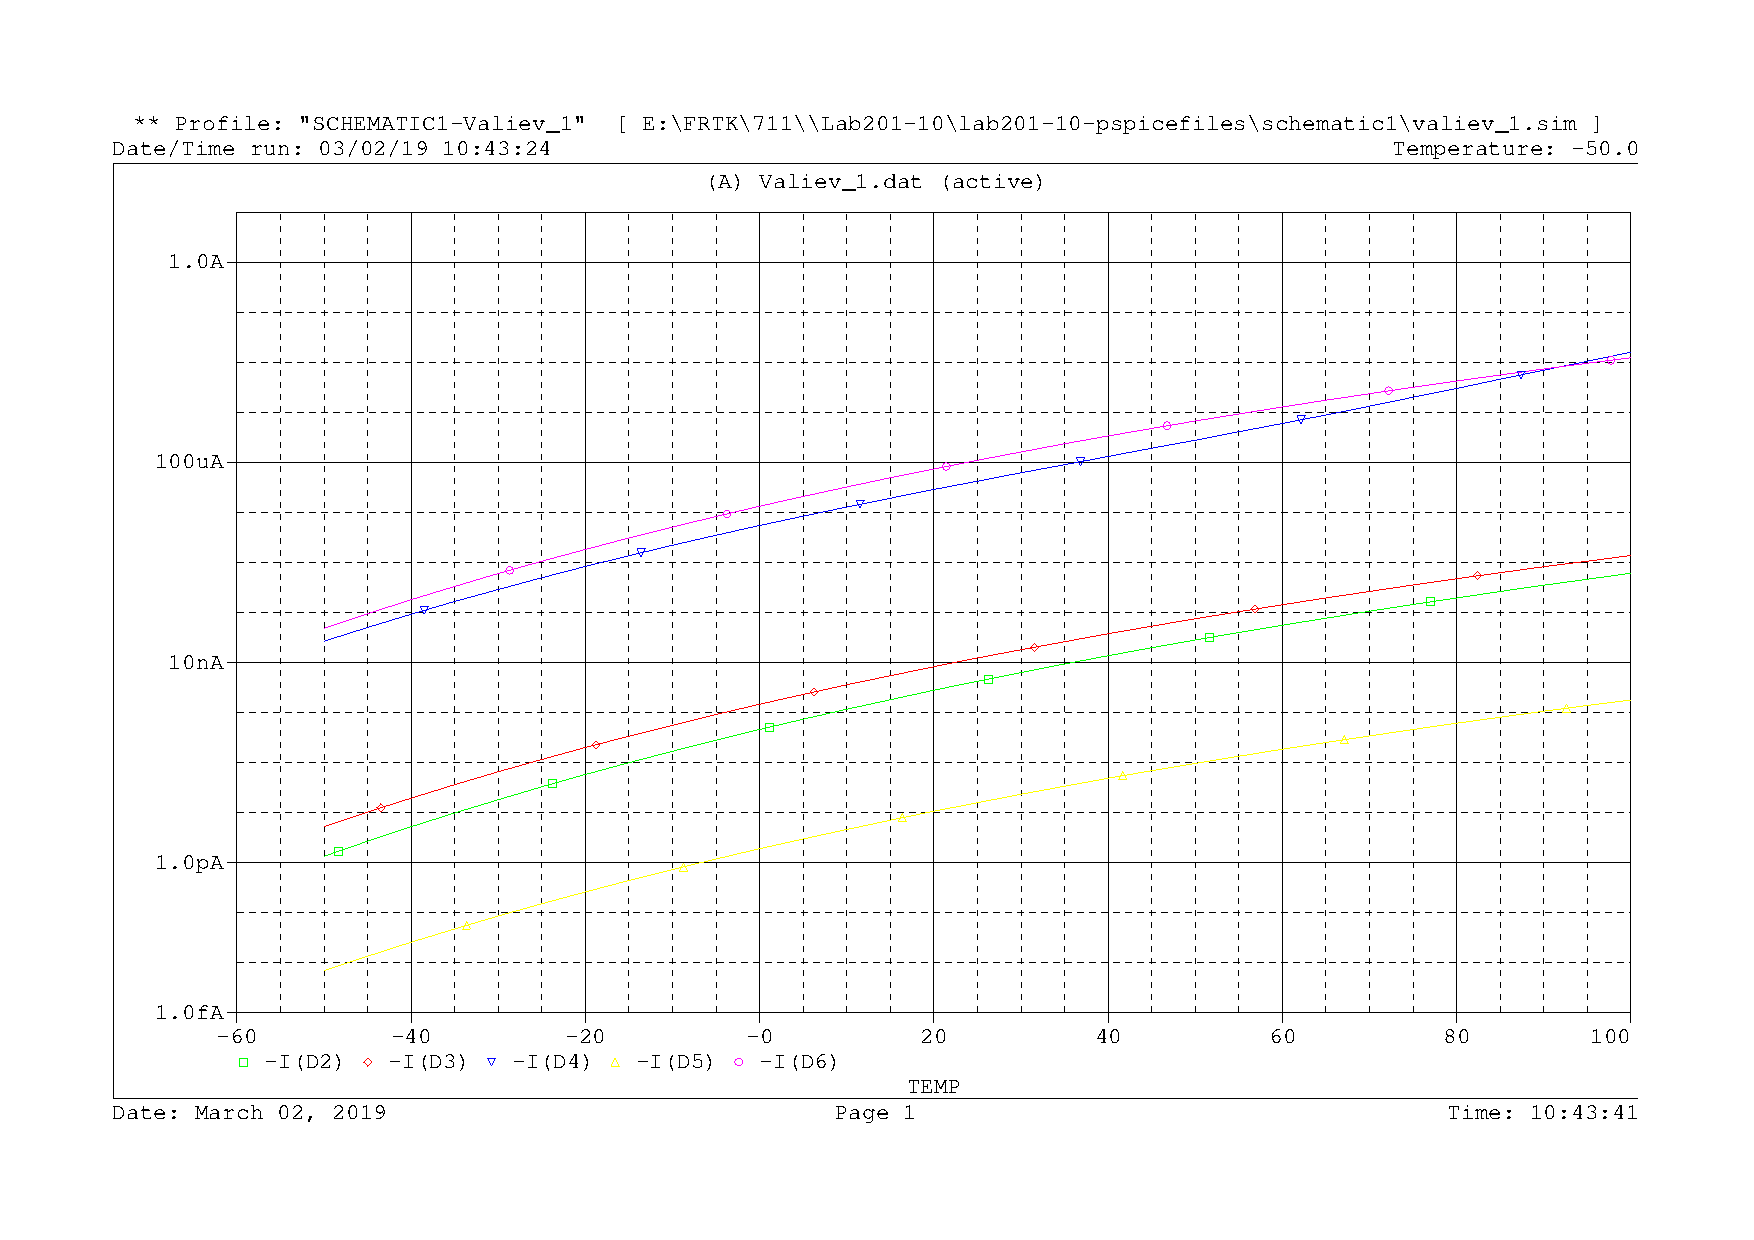
\includegraphics[width = 0.85 \textwidth]{33}
	\caption{Зависимости прямого тока от температуры в диапазоне от $ -50 \Cd $ до $ +100 \Cd $}
	\label{2.2.1}
\end{figure}

\textbf{{\normalsize 2.2.1.а.}}
Для импульсного ВЧ диода получим температурную зависимость относ. ТКПТ в области $ 17 \Cd < T < 47 \Cd $ при $ U_d = 0.6V $.
\begin{figure}[H]
	\centering
	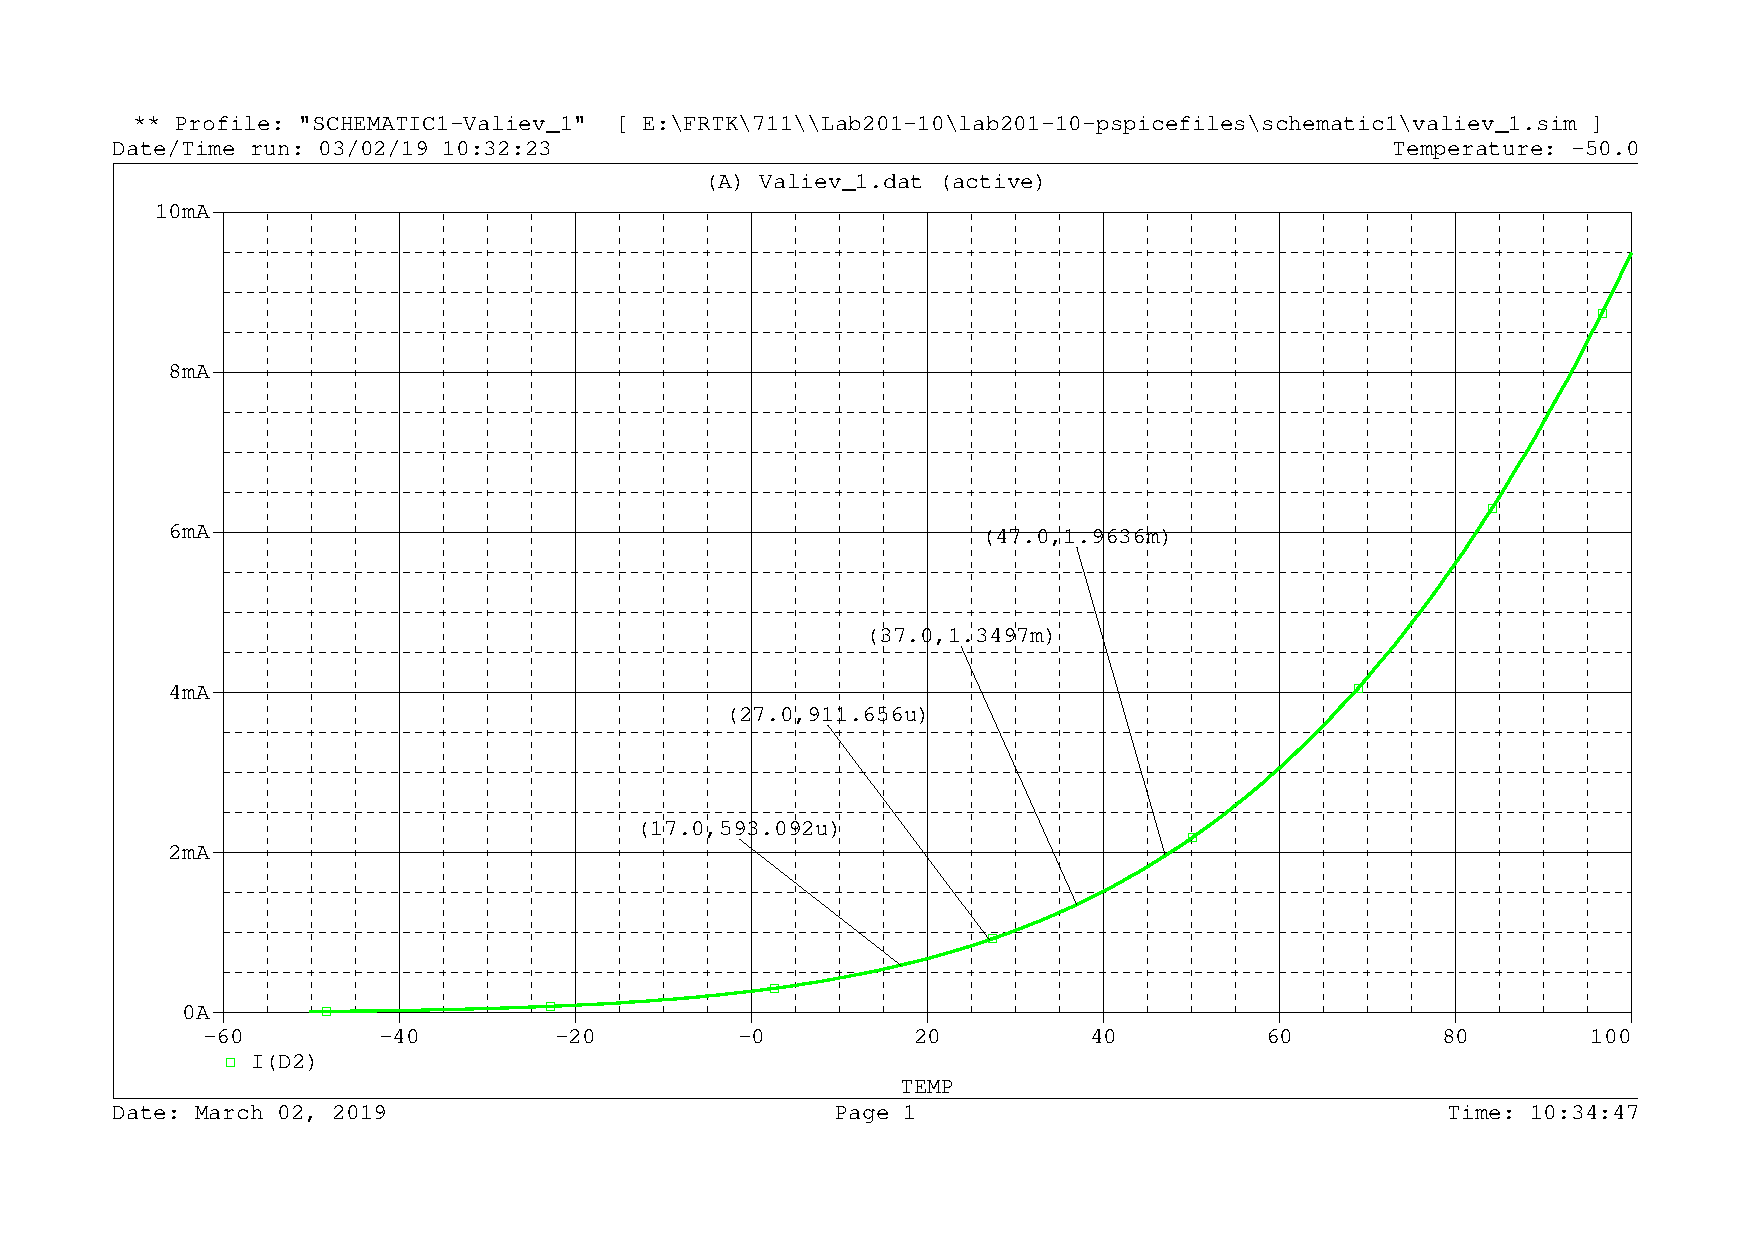
\includegraphics[width = 0.85 \textwidth]{31}
	\caption{D1N4149: при некоторых температурах}
	\label{2.2.1.1}
\end{figure}

\begin{figure}[H]
	\centering
	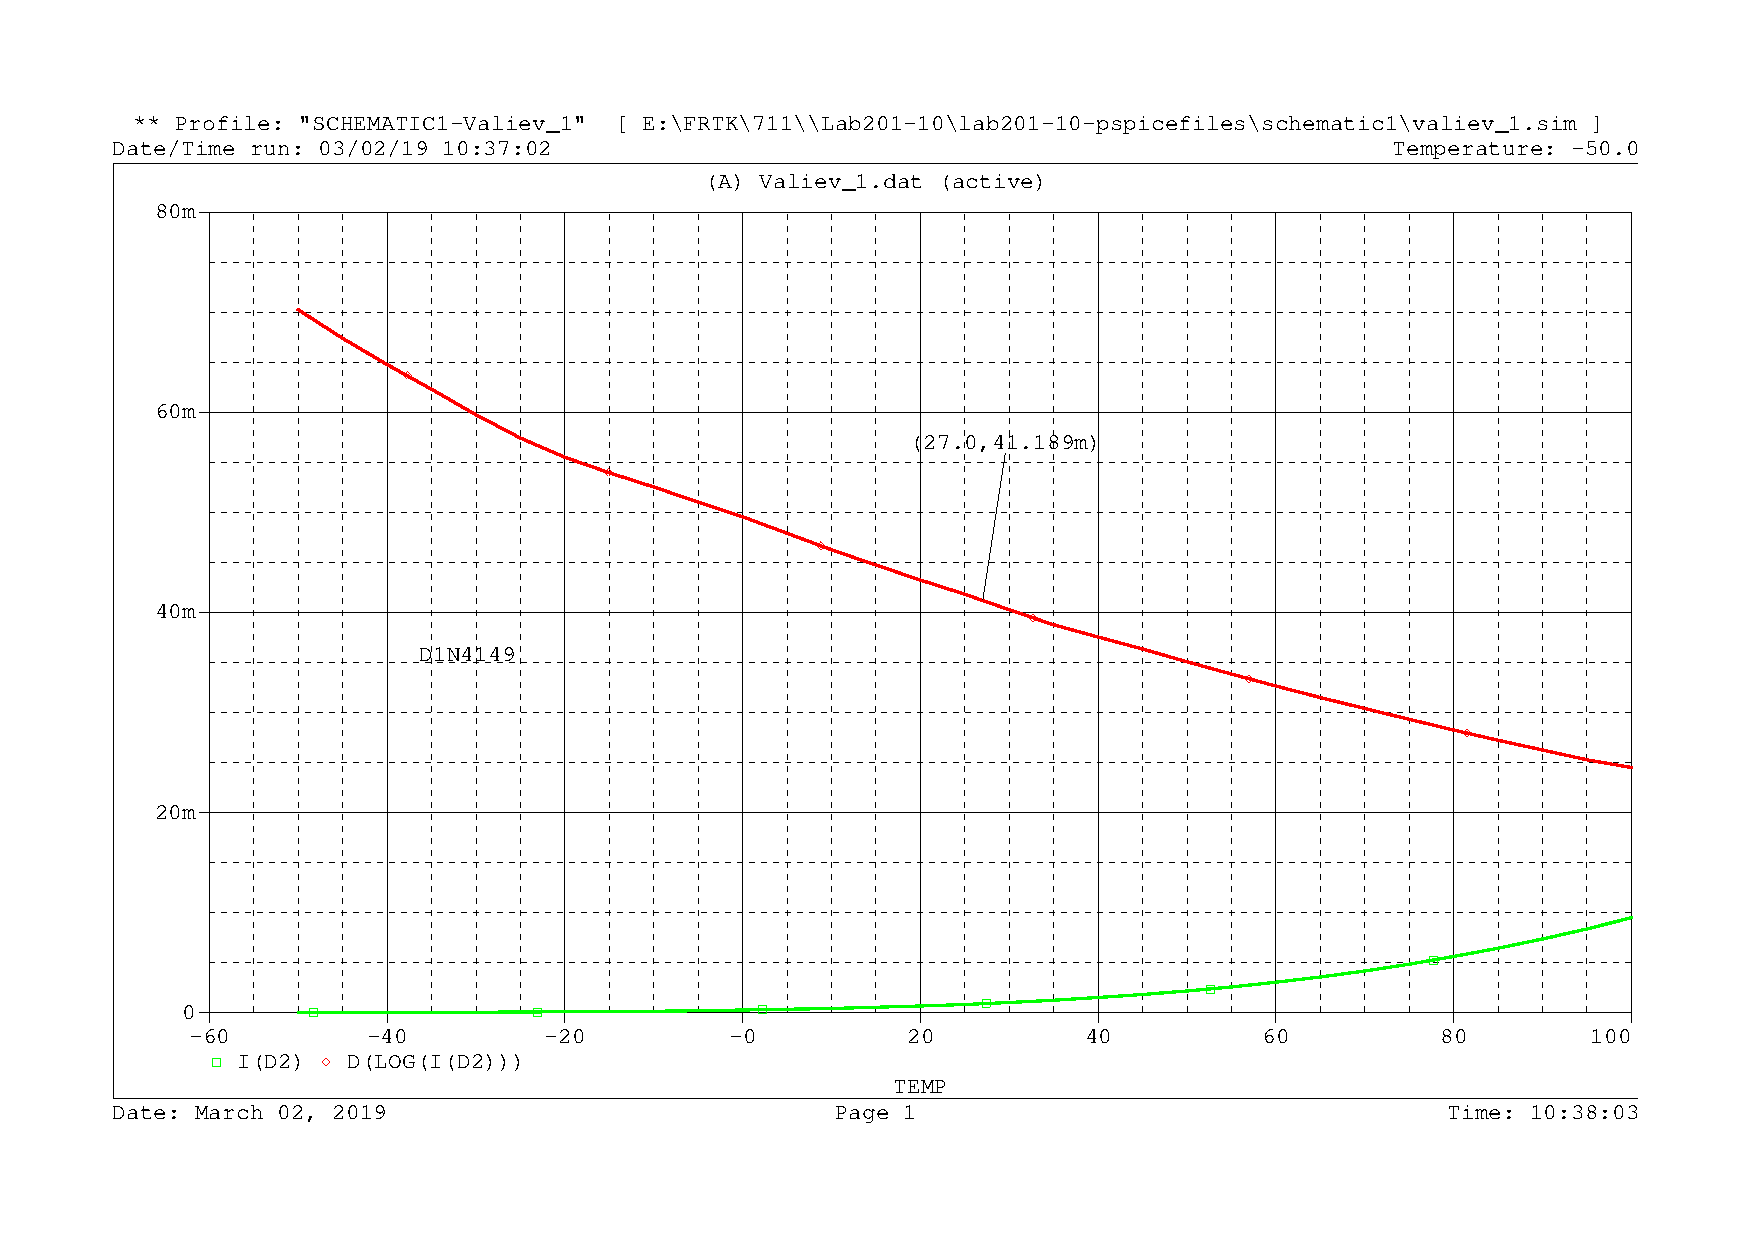
\includegraphics[width = 0.95 \textwidth]{32}
	\caption{D1N4149: $ относ. ТКПТ \approx 4.3\% $}
\end{figure}

\subsubsection*{Температурная зависимость обратного тока $ I_{обр} = f(T, U_d = const) $}

\textbf{{\normalsize 2.2.2.}}
Перевернем диоды обратной стороной, установим напряжение $ 1V $. Получим графики в логарифмическом масштабе зависимости обратных токов всех диодов.
\begin{figure}[H]
	\centering
	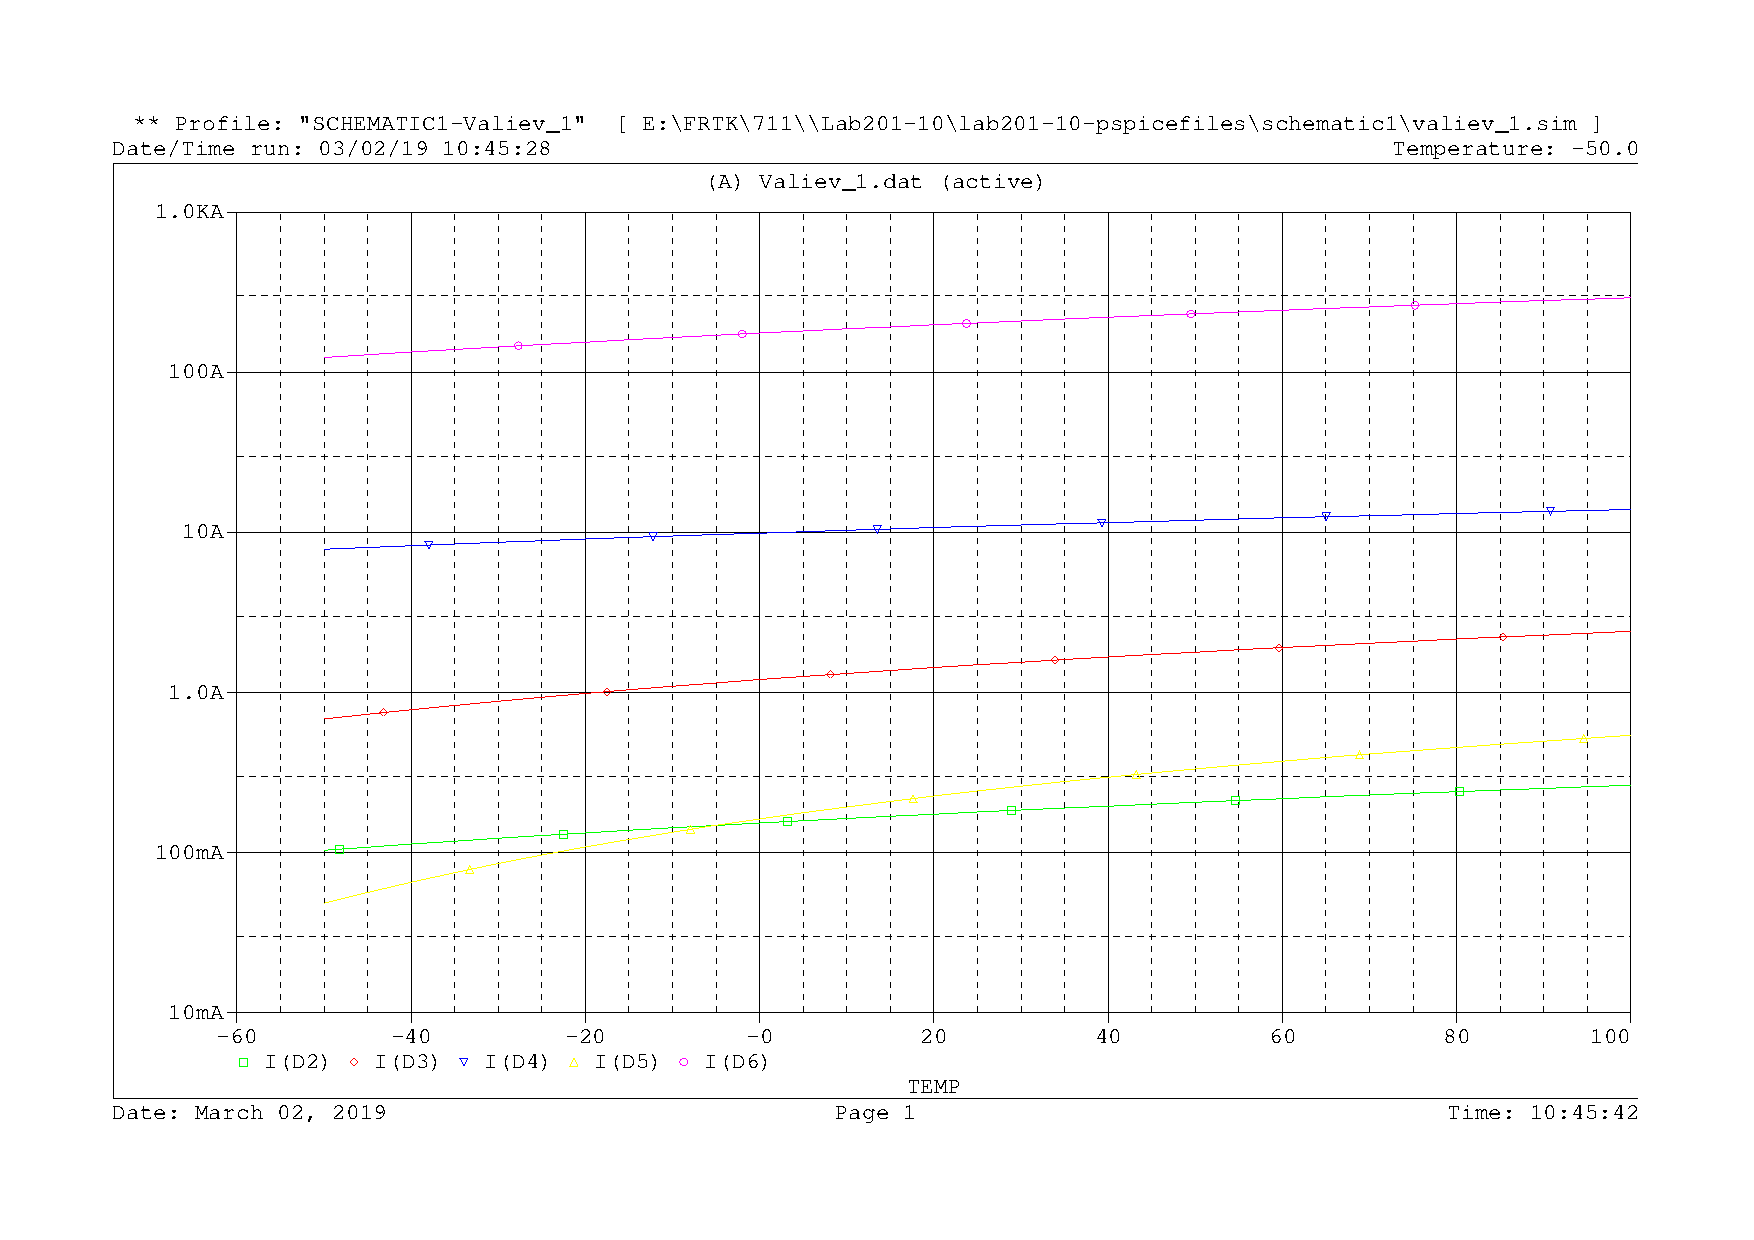
\includegraphics[width = 0.95\textwidth]{34}
	\caption{Зависимости обратных токов всех диодов}
	\label{2.2.2.}
\end{figure}

\textbf{{\normalsize 2.2.2.а.}}
Для импульсного ВЧ диода найдем значение обратного тока при $ T = 27 \Cd $.
\begin{figure}[H]
	\centering
	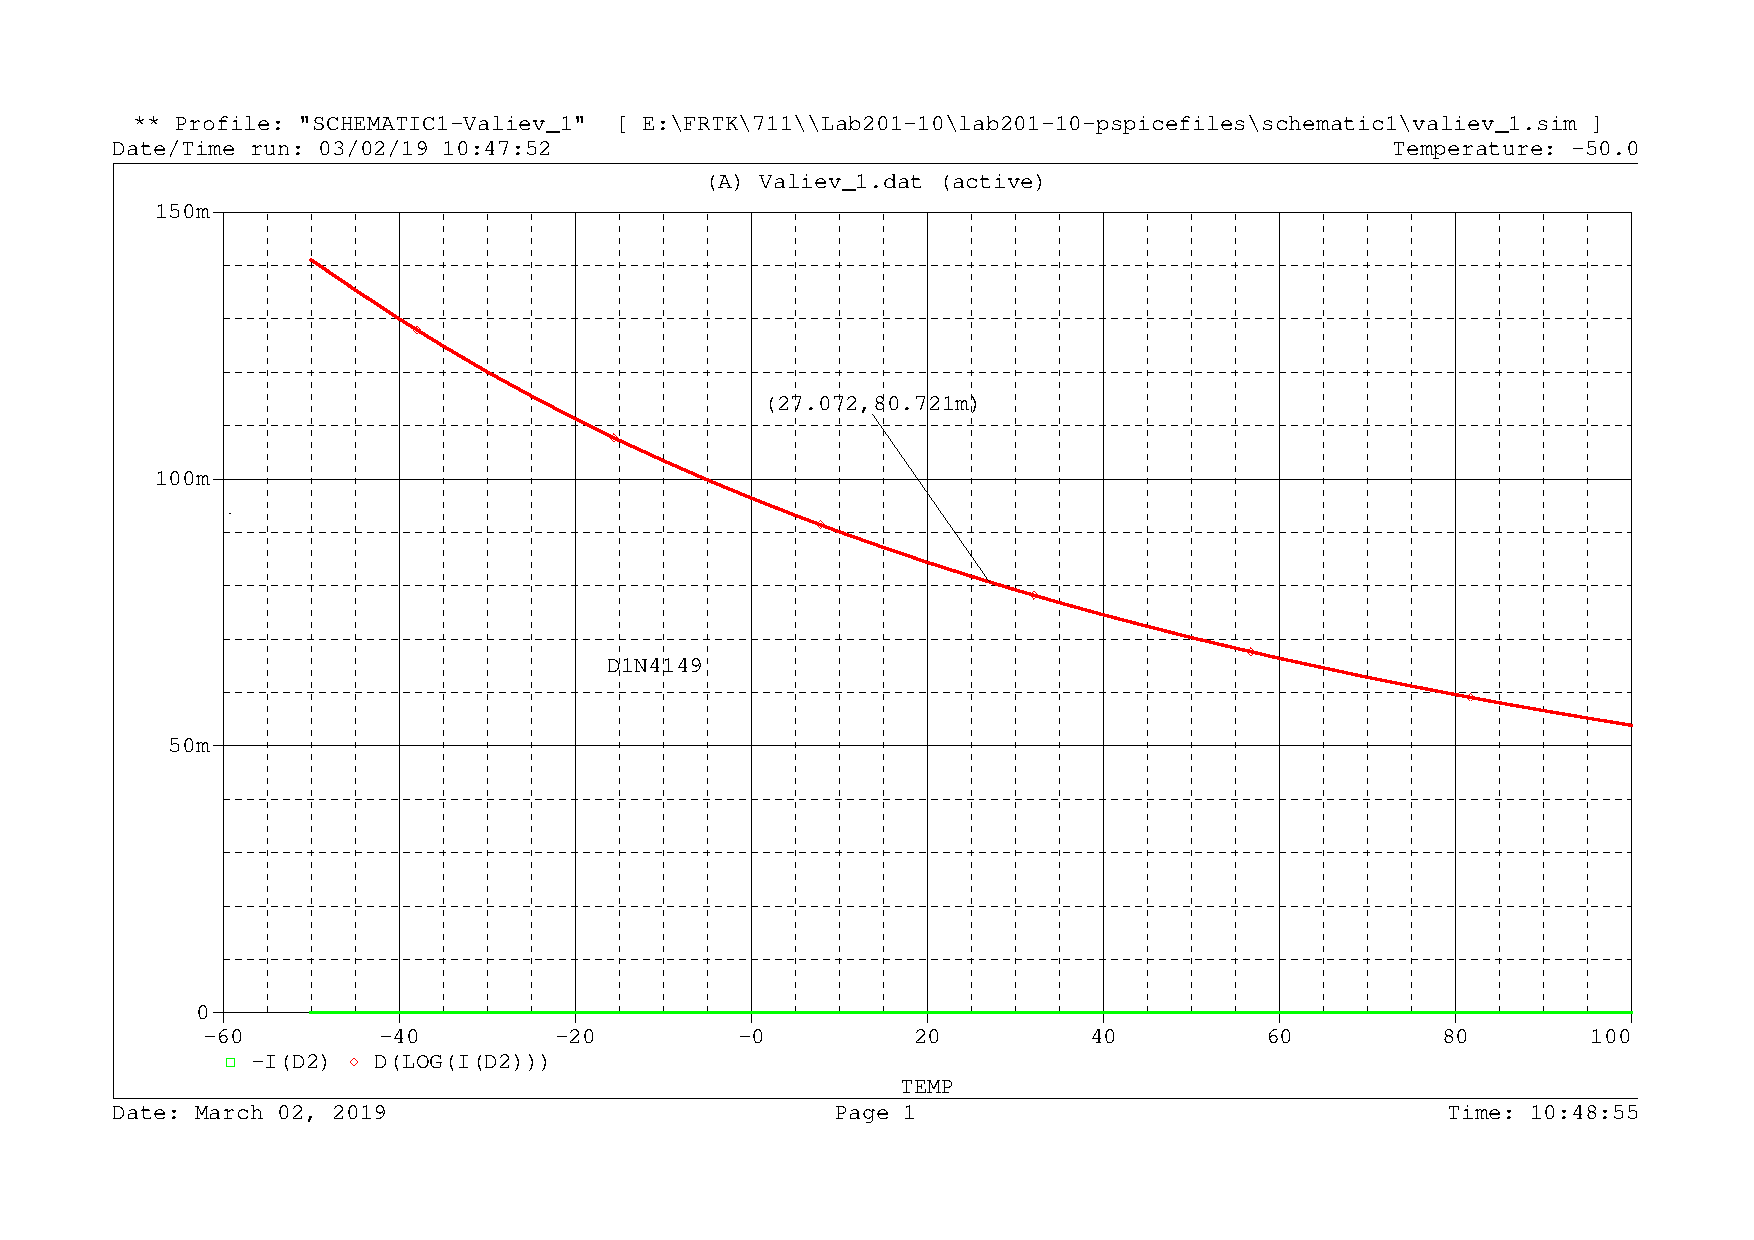
\includegraphics[width = 0.85 \textwidth]{35}
	\caption{Зависимости обратных токов всех диодов}
	\label{2.2.2.1.}
\end{figure}

\subsubsection*{Температурная зависимость прямого напряжения $ U_d = f(T, I_d = const) $}

\textbf{{\normalsize 2.2.3.}}
Соединим все диоды последовательно с источником тока $ 1mA $ как на рисунке $ \ref{scheme} $  получим графики зависимостей прямого напряжения на каждом диоде от температуры в диапазоне от $ -50 \Cd $ до $ 100 \Cd $.
\begin{figure}[H]
	\centering
	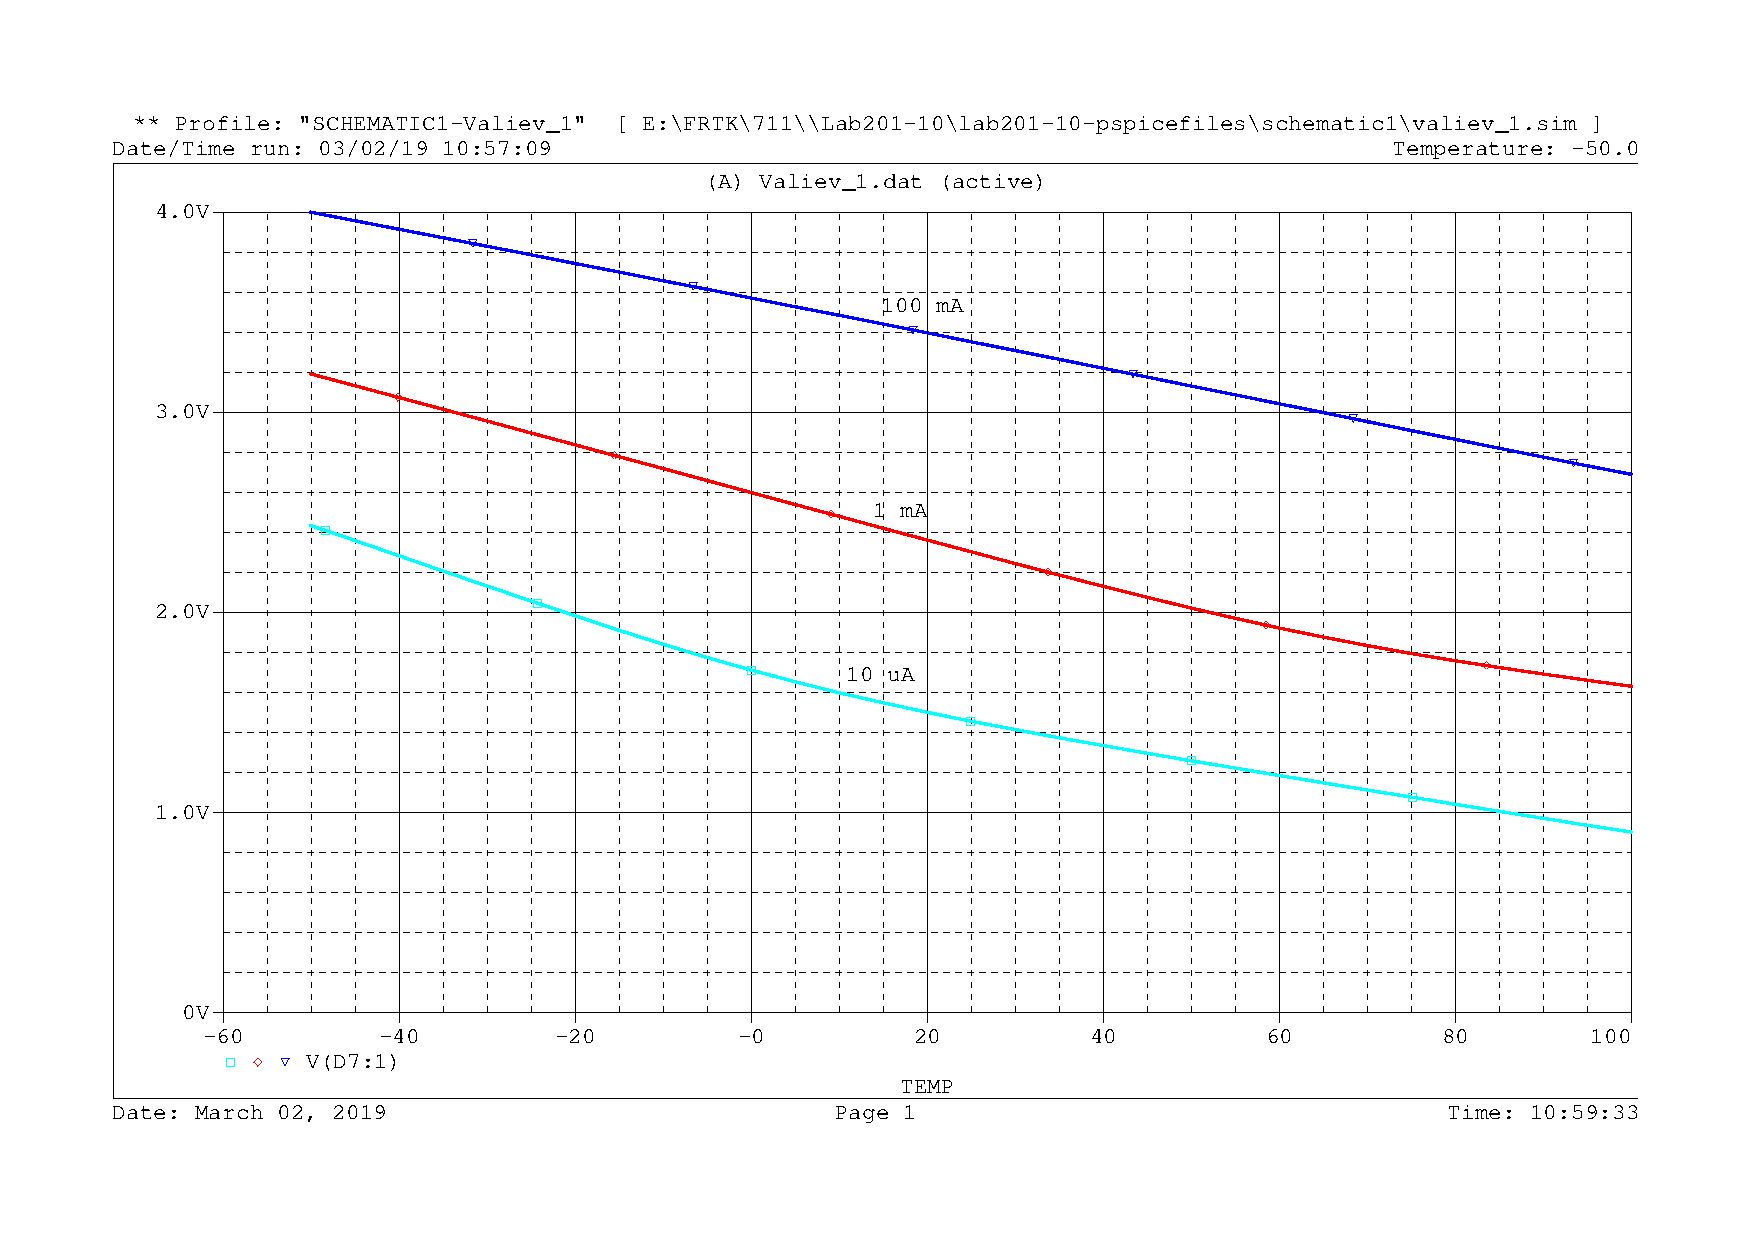
\includegraphics[width = 0.85 \textwidth]{37}
	\caption{D1N4149}
	\label{2.2.3.1}
\end{figure}
\begin{figure}[H]
	\centering
	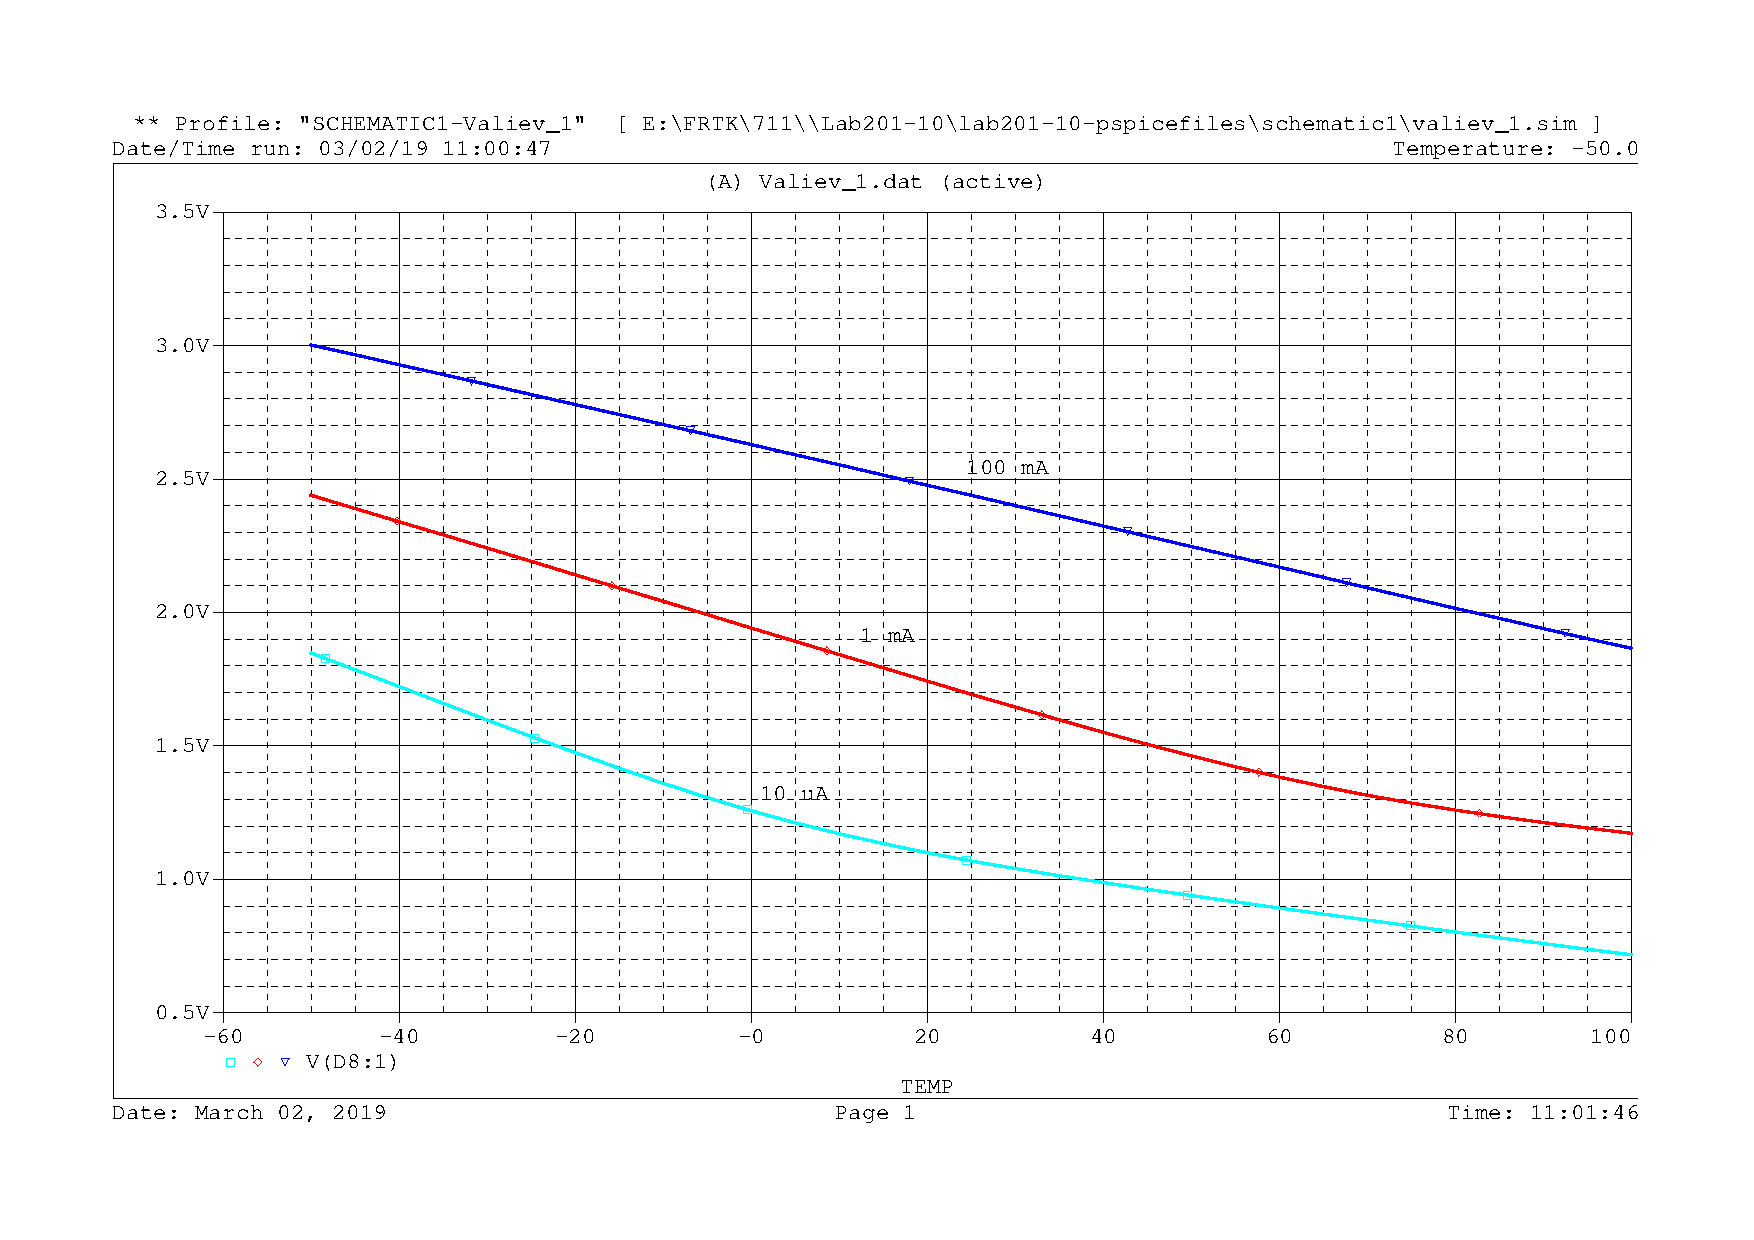
\includegraphics[width = \textwidth]{38}
	\caption{D1N4002}
	\label{2.2.3.2}
\end{figure}
\begin{figure}[H]
	\centering
	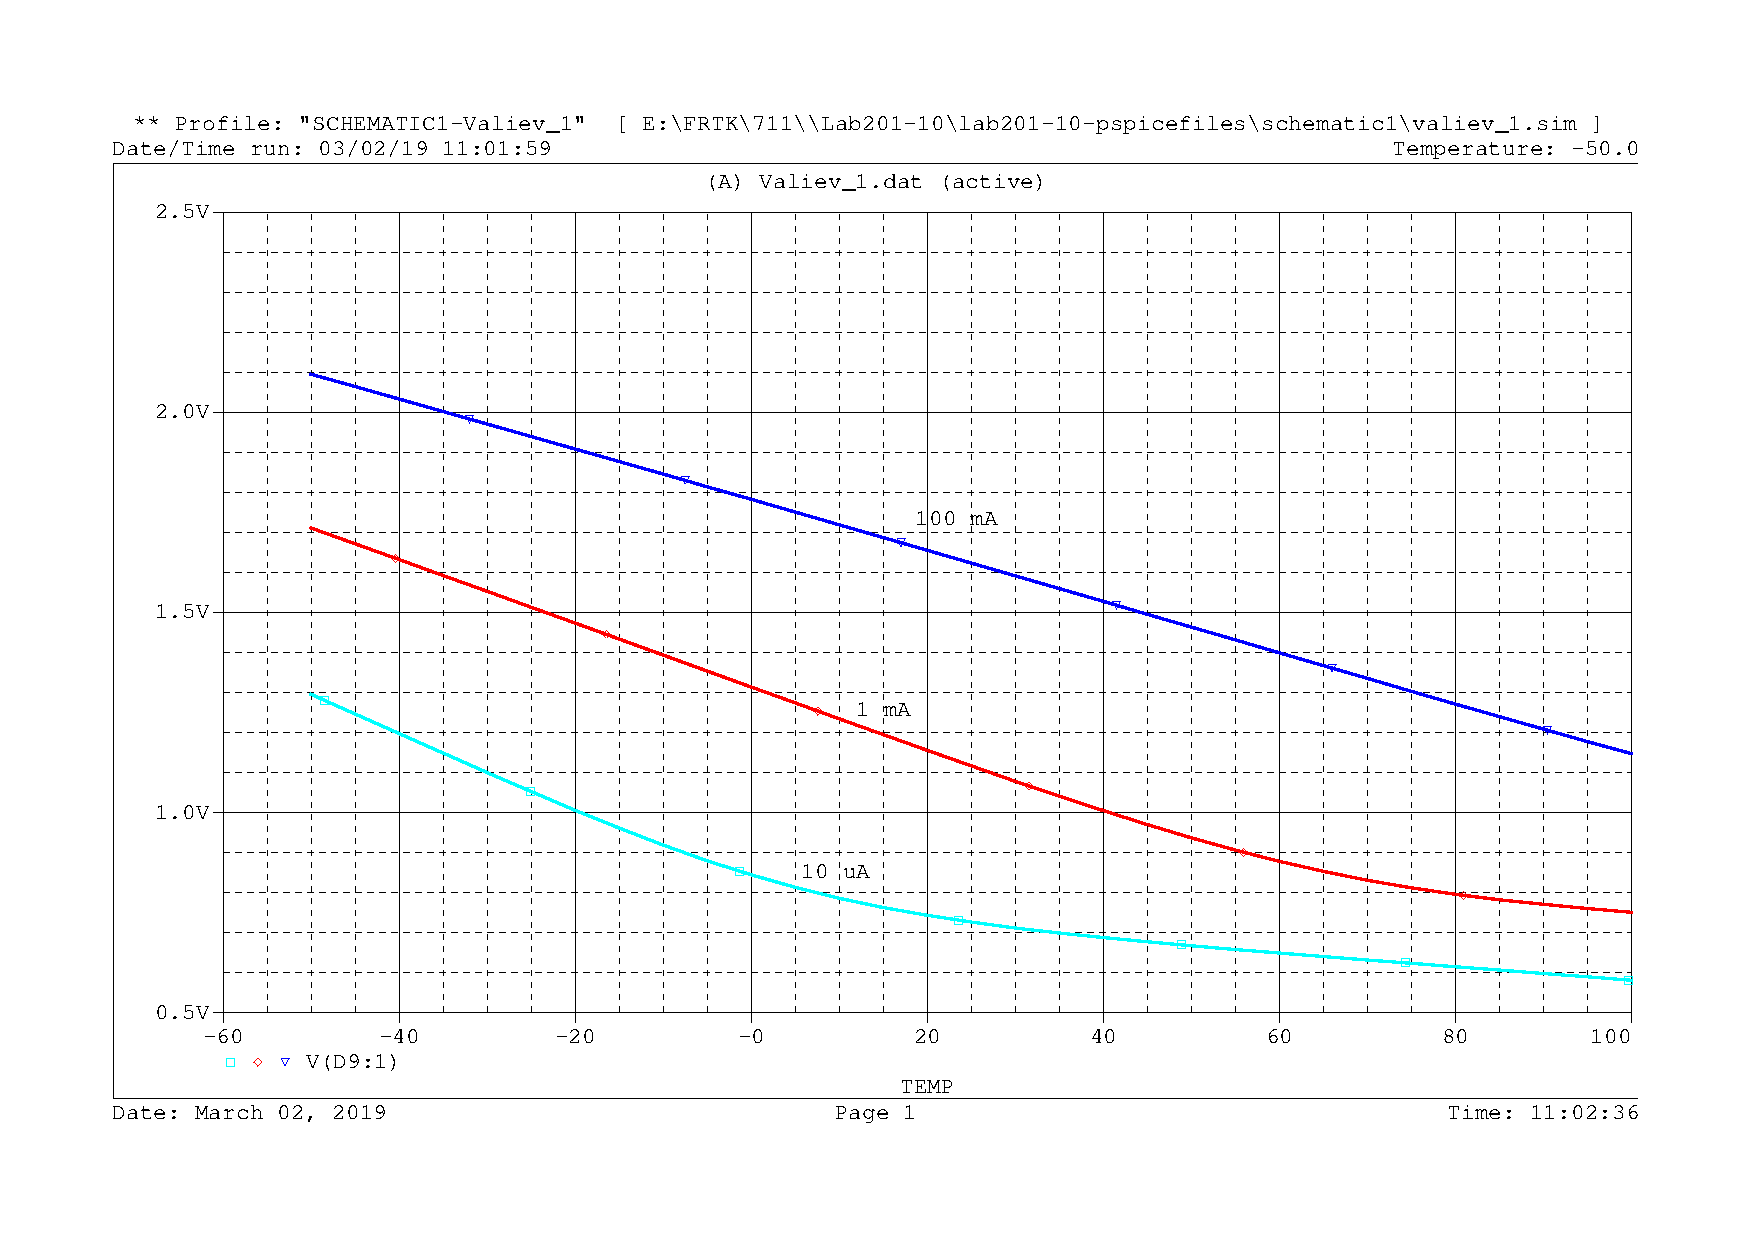
\includegraphics[width = \textwidth]{39}
	\caption{D1N5818}
	\label{2.2.3.3}
\end{figure}
\begin{figure}[H]
	\centering
	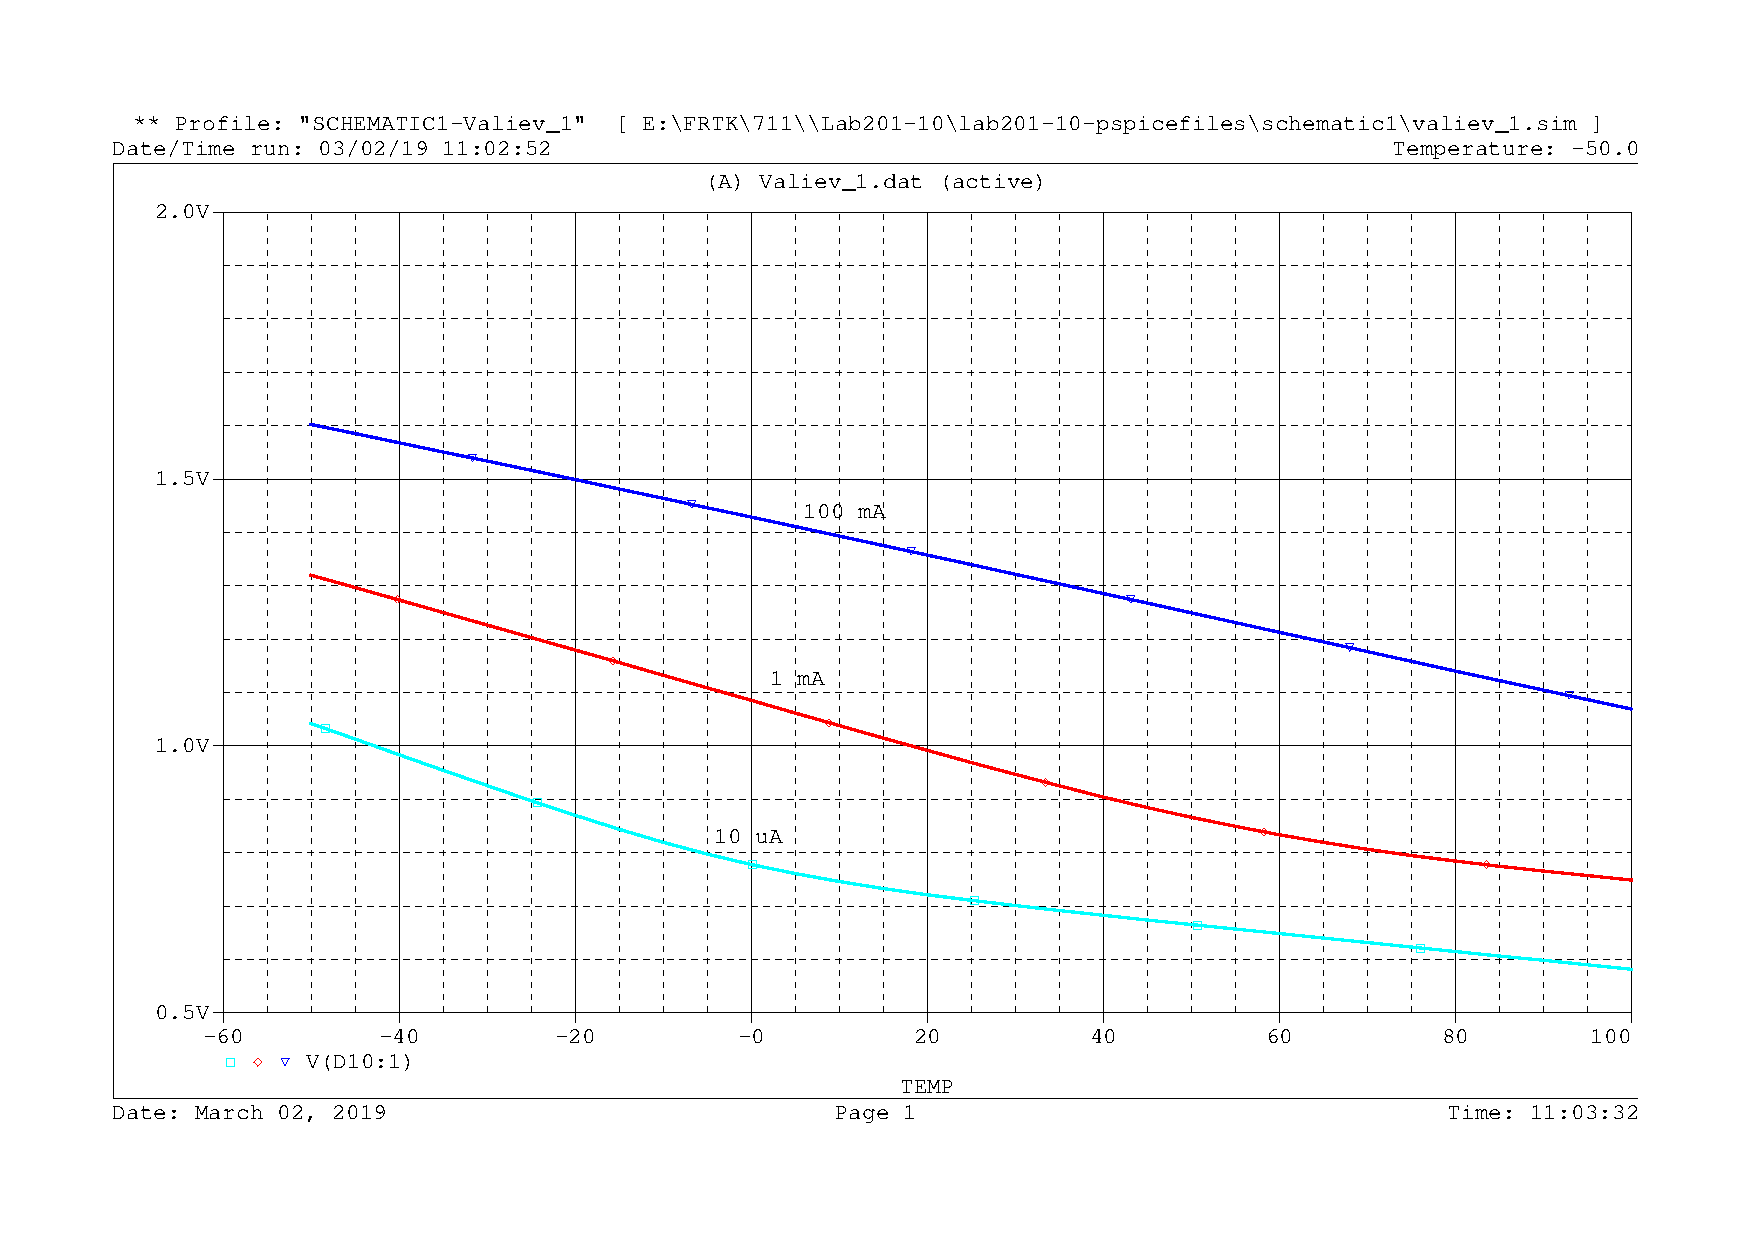
\includegraphics[width = \textwidth]{40}
	\caption{D1N5443A}
	\label{2.2.3.4}
\end{figure}
\begin{figure}[H]
	\centering
	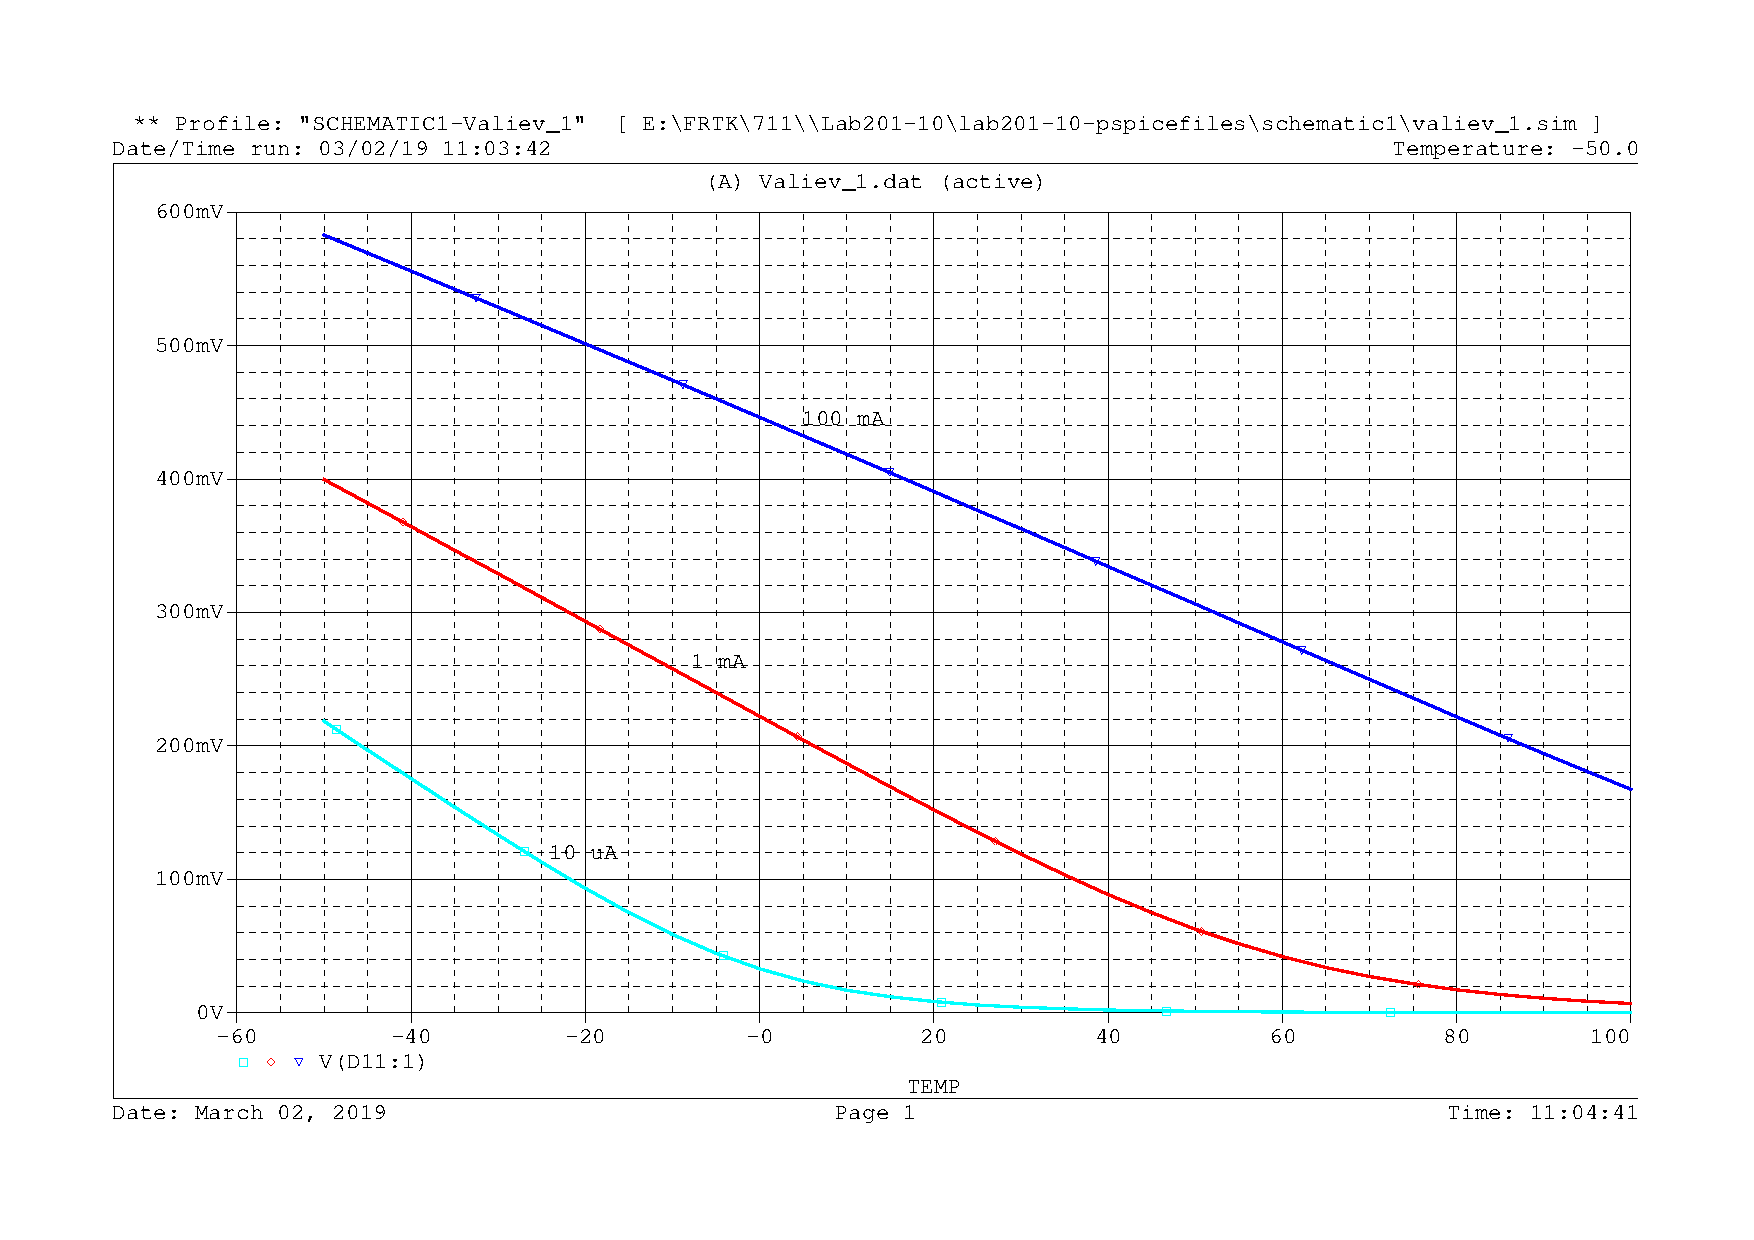
\includegraphics[width = \textwidth]{41}
	\caption{D04AZ2\_2}
	\label{2.2.3.5}
\end{figure}

\subsubsection*{Температурная зависимость напряжения пробоя стабилитрона}

\textbf{{\normalsize 2.2.4.}}
Повернем стабилитрон каком кверху к источнику тока и получим зависимость напряжения на стабилитроне от обратного тока $ U = f(I_{обр}, T = const) $ в диапазоне от $ (2-5) mA $ до $ (50 - 100)mA $ при значениях температуры: $ -40 \Cd, 27 \Cd, 85 \Cd $.\\

\textbf{{\normalsize 2.2.4.а.}}
Изобразим полученную зависимость на графике (рисунок $ \ref{2.2.4.} $).
\begin{figure}[H]
	\centering
	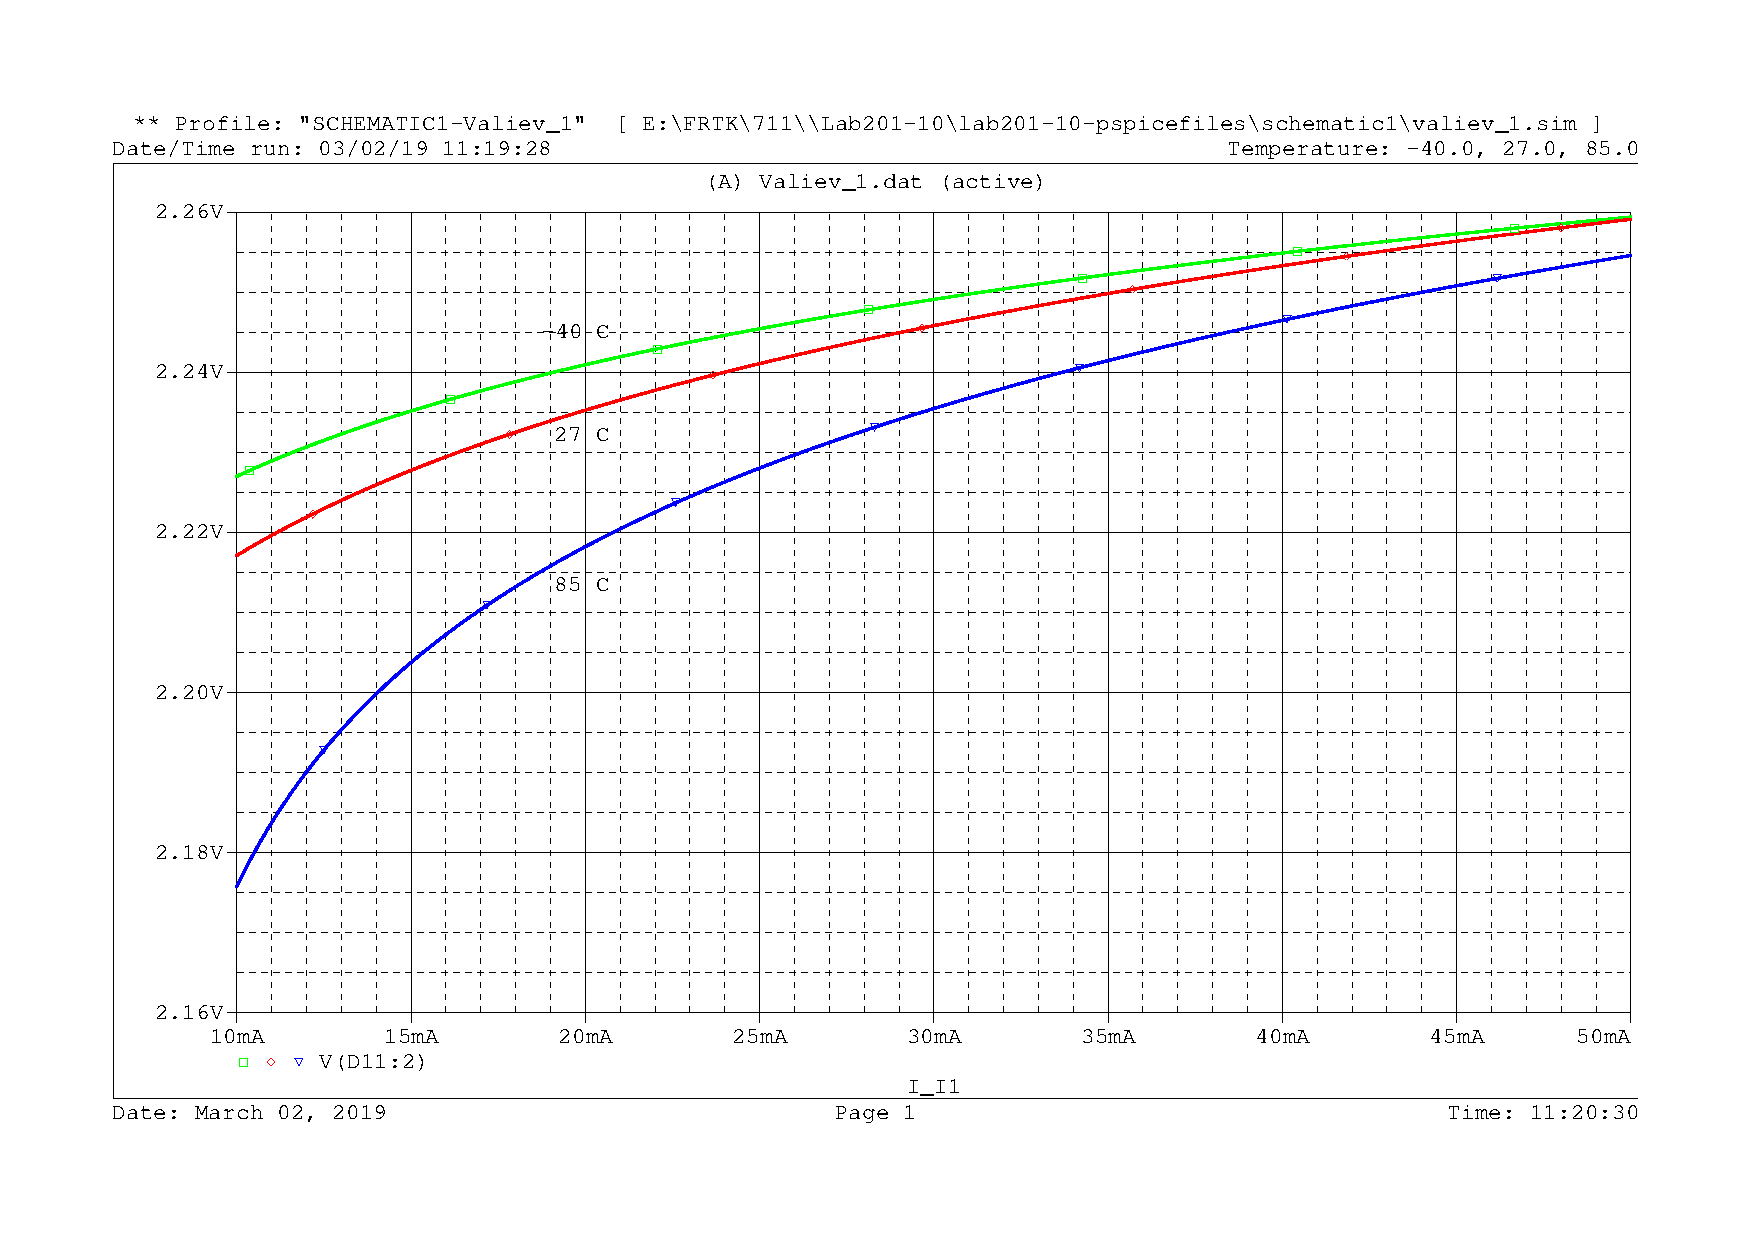
\includegraphics[width = \textwidth]{42}
	\caption{Стабилитрон}
	\label{2.2.4.}
\end{figure}

\newpage

\textbf{{\normalsize 2.2.4.б.}}
Для ВАХ с параметром $ T = 27 \Cd $ напечатаем на графике необходимые данные и определим величину абсолютного и относительного изменений (относительно паспортного значения $ U_{st} = Bv $) напряжения в использованном диапазоне $ \Delta I = (50-100) mA $ -- $ (2-5) mA $ изменений тока.

$$ \dfrac{\Delta U}{U_{st}} \cdot 100\% \approx 2.7\% $$

\begin{figure}[H]
	\centering
	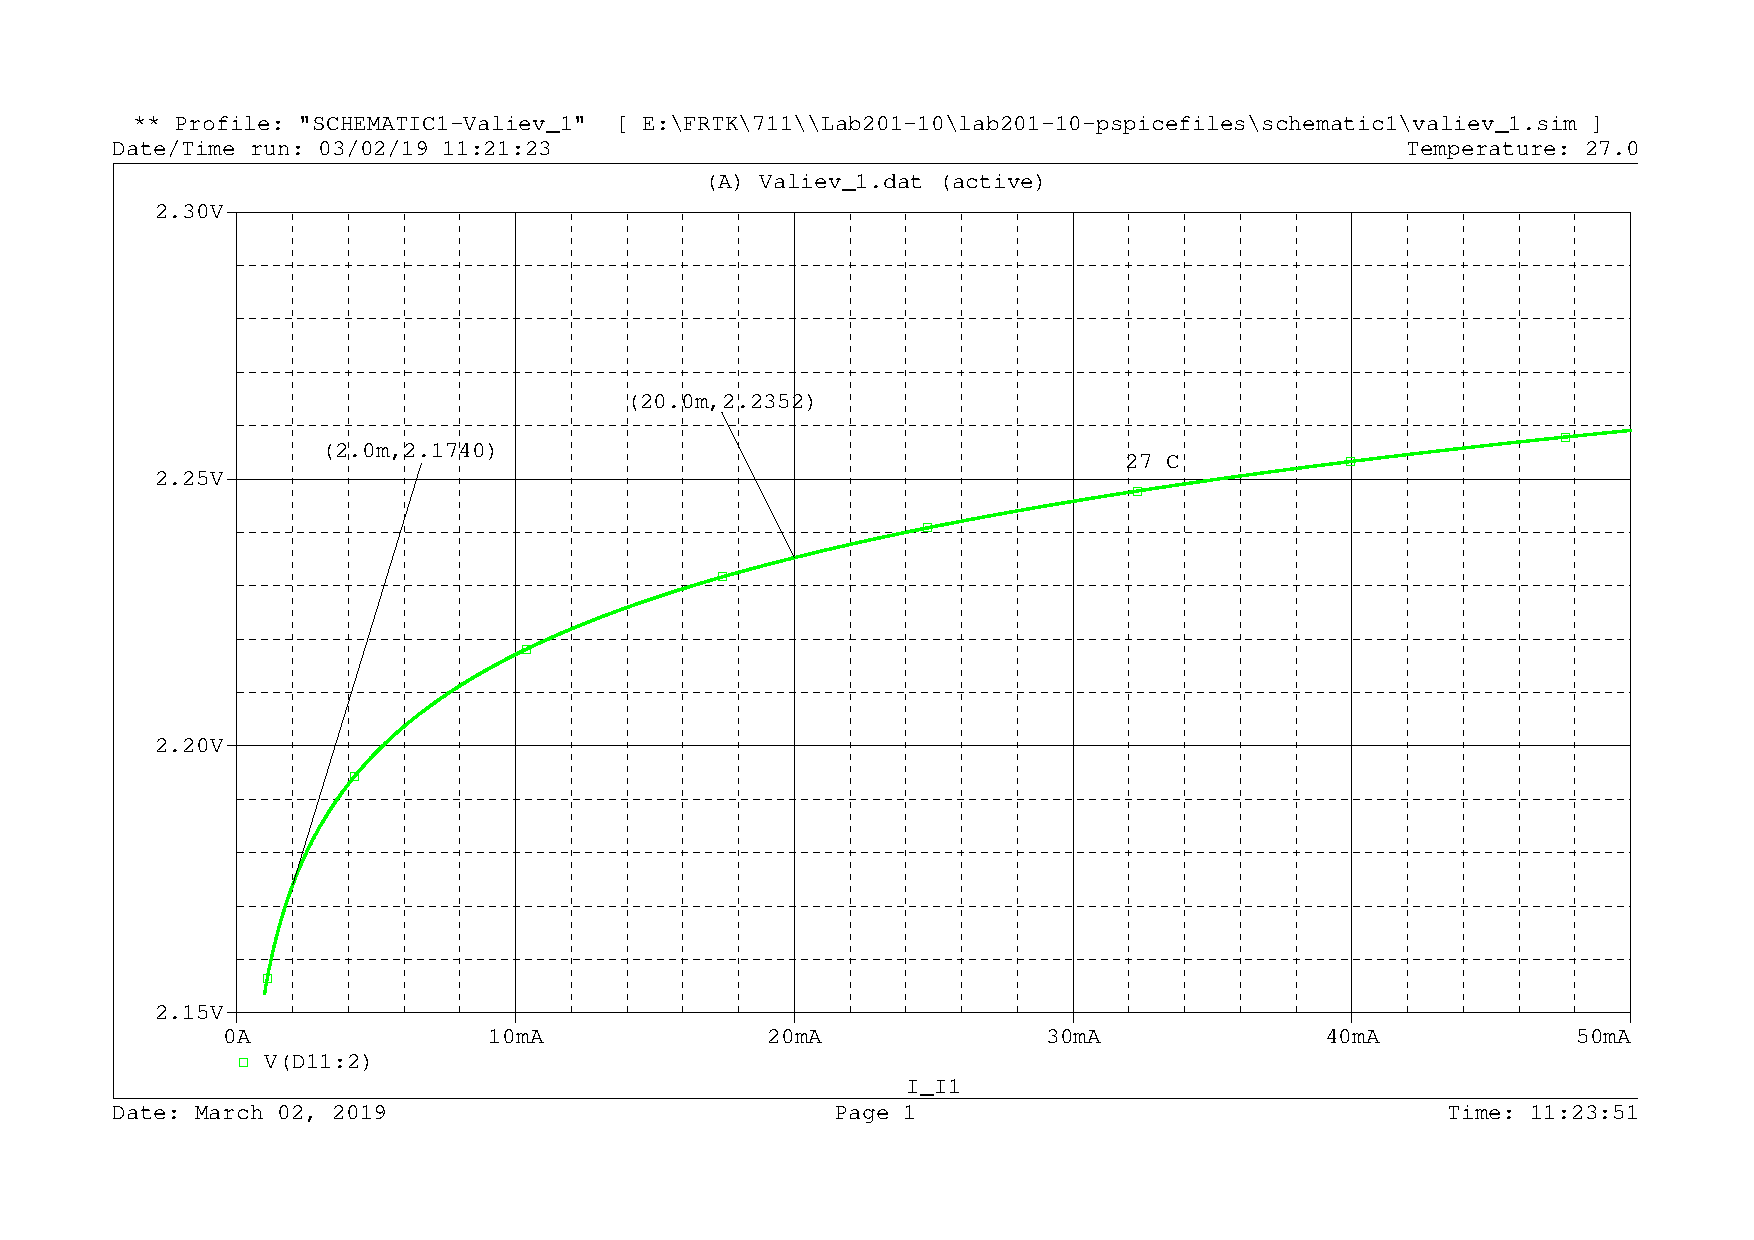
\includegraphics[width = \textwidth]{43}
	\caption{Стабилитрон при $ T = 27 \Cd $}
	\label{2.2.4.2}
\end{figure}

\newpage

\textbf{{\normalsize 2.2.4.в.}}
Получим зависимость дифференциального сопротивления стабилитрона от тока, а также найдем его значение при $ 10mA $.

\begin{figure}[H]
	\centering
	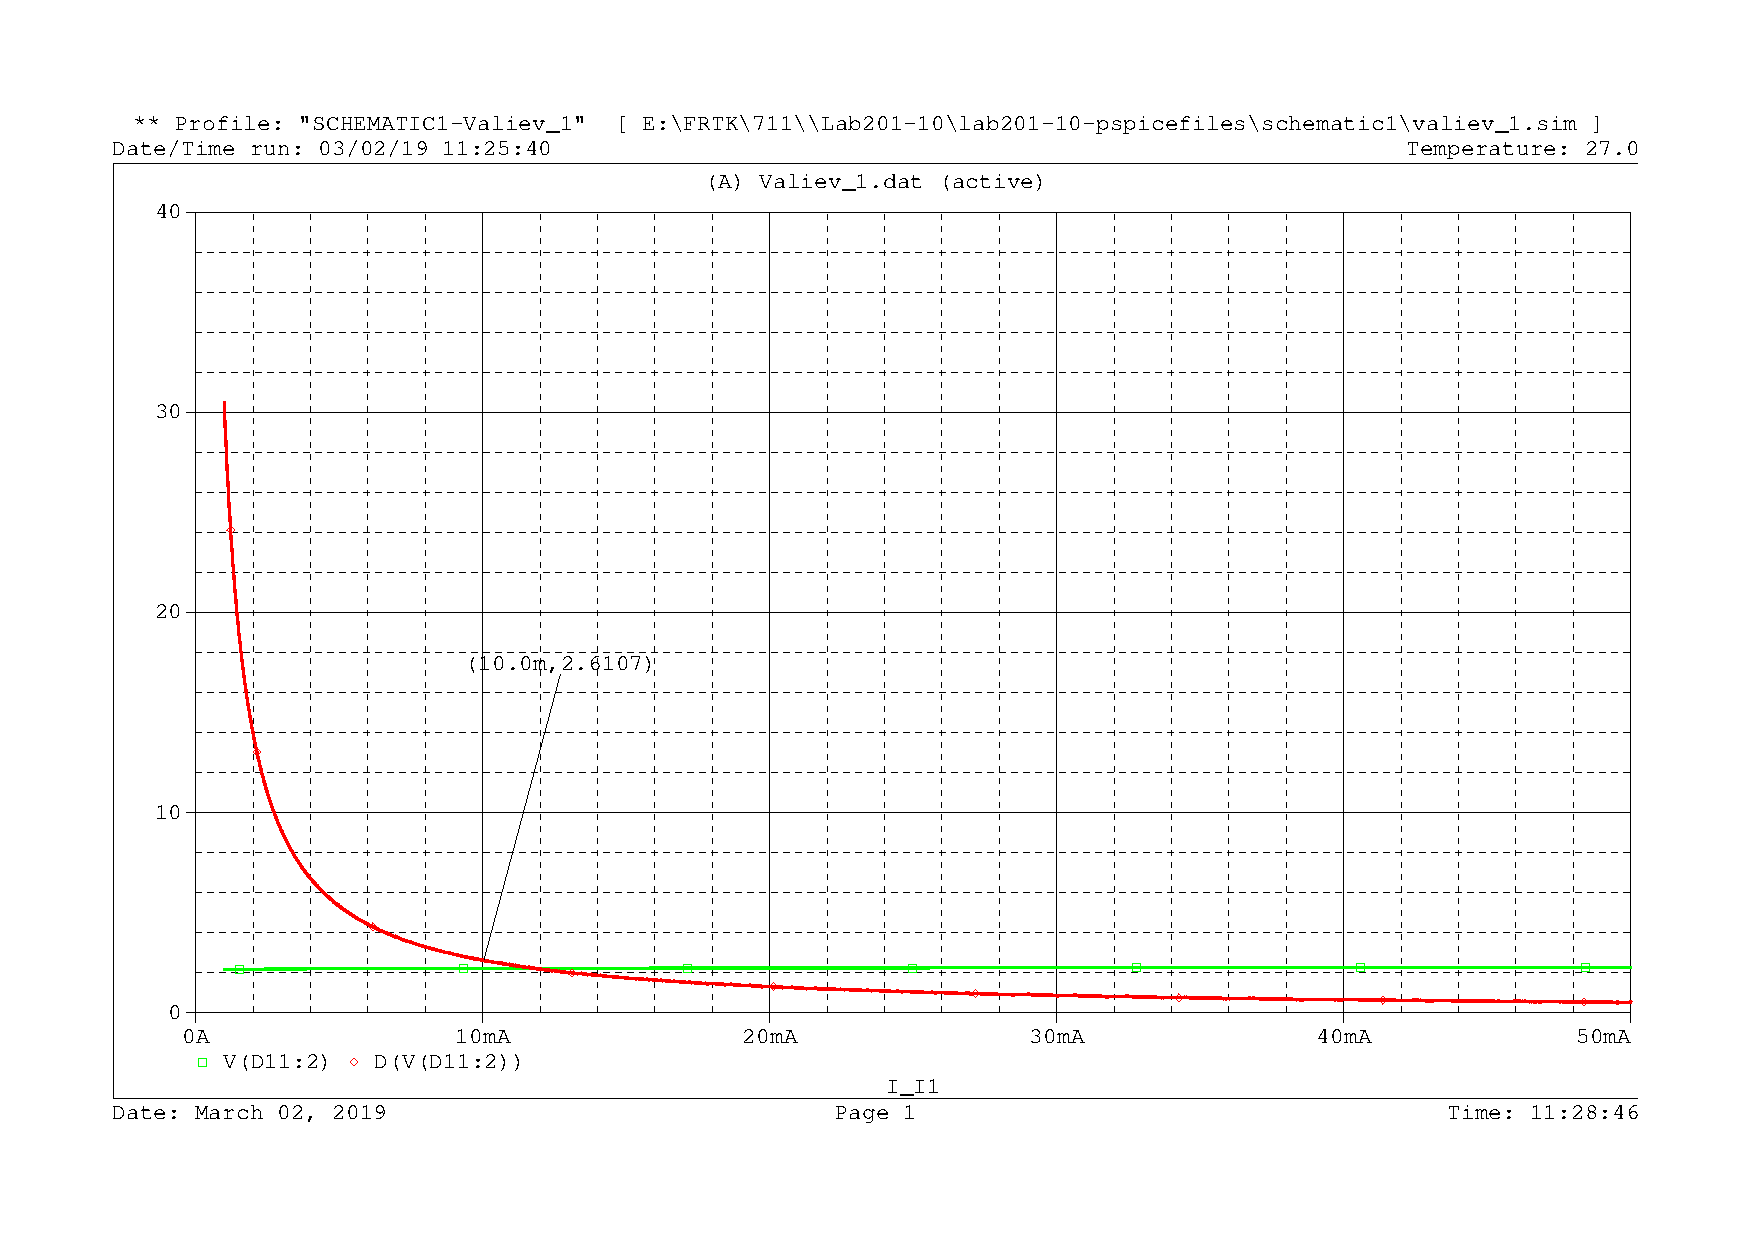
\includegraphics[width = \textwidth]{44}
	\caption{Стабилитрон и его дифференциальное сопротивление }
	\label{2.2.4.3}
\end{figure}

При $ I = 10mA $ получаем значение дифференциального сопротивления
$$ R(I=10mA) \approx 2.61 \Omega $$

\end{document}